%%%%%%%%%%%%%%%%%%%%%%%%%%%%%%%%%%%%%%%%%
% The Legrand Orange Book
% LaTeX Template
% Version 2.4 (26/09/2018)
%
% This template was downloaded from:
% http://www.LaTeXTemplates.com
%
% Original author:
% Mathias Legrand (legrand.mathias@gmail.com) with modifications by:
% Vel (vel@latextemplates.com)
%
% License:
% CC BY-NC-SA 3.0 (http://creativecommons.org/licenses/by-nc-sa/3.0/)
%
% Compiling this template:
% This template uses biber for its bibliography and makeindex for its index.
% When you first open the template, compile it from the command line with the 
% commands below to make sure your LaTeX distribution is configured correctly:
%
% 1) pdflatex main
% 2) makeindex main.idx -s StyleInd.ist
% 3) biber main
% 4) pdflatex main x 2
%
% After this, when you wish to update the bibliography/index use the appropriate
% command above and make sure to compile with pdflatex several times 
% afterwards to propagate your changes to the document.
%
% This template also uses a number of packages which may need to be
% updated to the newest versions for the template to compile. It is strongly
% recommended you update your LaTeX distribution if you have any
% compilation errors.
%
% Important note:
% Chapter heading images should have a 2:1 width:height ratio,
% e.g. 920px width and 460px height.
%
%%%%%%%%%%%%%%%%%%%%%%%%%%%%%%%%%%%%%%%%%

%----------------------------------------------------------------------------------------
%	PACKAGES AND OTHER DOCUMENT CONFIGURATIONS
%----------------------------------------------------------------------------------------

\documentclass[11pt,fleqn]{book} % Default font size and left-justified equations

%%%%%%%%%%%%%%%%%%%%%%%%%%%%%%%%%%%%%%%%%
% The Legrand Orange Book
% Structural Definitions File
% Version 2.1 (26/09/2018)
%
% Original author:
% Mathias Legrand (legrand.mathias@gmail.com) with modifications by:
% Vel (vel@latextemplates.com)
% 
% This file was downloaded from:
% http://www.LaTeXTemplates.com
%
% License:
% CC BY-NC-SA 3.0 (http://creativecommons.org/licenses/by-nc-sa/3.0/)
%
%%%%%%%%%%%%%%%%%%%%%%%%%%%%%%%%%%%%%%%%%

%----------------------------------------------------------------------------------------
%	VARIOUS REQUIRED PACKAGES AND CONFIGURATIONS
%----------------------------------------------------------------------------------------

\usepackage{graphicx} % Required for including pictures
\graphicspath{{Pictures/}} % Specifies the directory where pictures are stored

\usepackage{lipsum} % Inserts dummy text

\usepackage{tikz} % Required for drawing custom shapes
\usetikzlibrary{shapes.geometric, arrows}

% tekið út \usepackage[english]{babel} % English language/hyphenation

\usepackage{enumitem} % Customize lists
\setlist{nolistsep} % Reduce spacing between bullet points and numbered lists

\usepackage{booktabs} % Required for nicer horizontal rules in tables

\usepackage{xcolor} % Required for specifying colors by name
\definecolor{ocre}{RGB}{34,139,34} % Define the orange color used for highlighting throughout the book

%----------------------------------------------------------------------------------------
%	MARGINS
%----------------------------------------------------------------------------------------

\usepackage{geometry} % Required for adjusting page dimensions and margins

\geometry{
	paper=a4paper, % Paper size, change to letterpaper for US letter size
	top=3cm, % Top margin
	bottom=3cm, % Bottom margin
	left=3cm, % Left margin
	right=3cm, % Right margin
	headheight=14pt, % Header height
	footskip=1.4cm, % Space from the bottom margin to the baseline of the footer
	headsep=10pt, % Space from the top margin to the baseline of the header
	%showframe, % Uncomment to show how the type block is set on the page
}

%----------------------------------------------------------------------------------------
%	FONTS
%----------------------------------------------------------------------------------------

\usepackage{avant} % Use the Avantgarde font for headings
%\usepackage{times} % Use the Times font for headings
\usepackage{mathptmx} % Use the Adobe Times Roman as the default text font together with math symbols from the Sym­bol, Chancery and Com­puter Modern fonts

\usepackage{microtype} % Slightly tweak font spacing for aesthetics
\usepackage[utf8]{inputenc} % Required for including letters with accents
\usepackage[T1]{fontenc} % Use 8-bit encoding that has 256 glyphs

%\usepackage[icelandic]{babel}

%----------------------------------------------------------------------------------------
%	BIBLIOGRAPHY AND INDEX
%----------------------------------------------------------------------------------------

%\usepackage[style=numeric,citestyle=numeric,sorting=nyt,sortcites=true,autopunct=true,babel=hyphen,hyperref=true,abbreviate=false,backref=true,backend=biber]{biblatex}
%\addbibresource{bibliography.bib} % BibTeX bibliography file
%\defbibheading{bibempty}{}

\usepackage{calc} % For simpler calculation - used for spacing the index letter headings correctly
\usepackage{makeidx} % Required to make an index
\makeindex % Tells LaTeX to create the files required for indexing

%----------------------------------------------------------------------------------------
%	MAIN TABLE OF CONTENTS
%----------------------------------------------------------------------------------------

\usepackage{titletoc} % Required for manipulating the table of contents

\contentsmargin{0cm} % Removes the default margin

% Part text styling (this is mostly taken care of in the PART HEADINGS section of this file)
\titlecontents{part}
	[0cm] % Left indentation
	{\addvspace{20pt}\bfseries} % Spacing and font options for parts
	{}
	{}
	{}

% Chapter text styling
\titlecontents{chapter}
	[1.25cm] % Left indentation
	{\addvspace{12pt}\large\sffamily\bfseries} % Spacing and font options for chapters
	{\color{ocre!60}\contentslabel[\Large\thecontentslabel]{1.25cm}\color{ocre}} % Formatting of numbered sections of this type
	{\color{ocre}} % Formatting of numberless sections of this type
	{\color{ocre!60}\normalsize\;\titlerule*[.5pc]{.}\;\thecontentspage} % Formatting of the filler to the right of the heading and the page number

% Section text styling
\titlecontents{section}
	[1.25cm] % Left indentation
	{\addvspace{3pt}\sffamily\bfseries} % Spacing and font options for sections
	{\contentslabel[\thecontentslabel]{1.25cm}} % Formatting of numbered sections of this type
	{} % Formatting of numberless sections of this type
	{\hfill\color{black}\thecontentspage} % Formatting of the filler to the right of the heading and the page number

% Subsection text styling
\titlecontents{subsection}
	[1.25cm] % Left indentation
	{\addvspace{1pt}\sffamily\small} % Spacing and font options for subsections
	{\contentslabel[\thecontentslabel]{1.25cm}} % Formatting of numbered sections of this type
	{} % Formatting of numberless sections of this type
	{\ \titlerule*[.5pc]{.}\;\thecontentspage} % Formatting of the filler to the right of the heading and the page number

% Figure text styling
\titlecontents{figure}
	[1.25cm] % Left indentation
	{\addvspace{1pt}\sffamily\small} % Spacing and font options for figures
	{\thecontentslabel\hspace*{1em}} % Formatting of numbered sections of this type
	{} % Formatting of numberless sections of this type
	{\ \titlerule*[.5pc]{.}\;\thecontentspage} % Formatting of the filler to the right of the heading and the page number

% Table text styling
\titlecontents{table}
	[1.25cm] % Left indentation
	{\addvspace{1pt}\sffamily\small} % Spacing and font options for tables
	{\thecontentslabel\hspace*{1em}} % Formatting of numbered sections of this type
	{} % Formatting of numberless sections of this type
	{\ \titlerule*[.5pc]{.}\;\thecontentspage} % Formatting of the filler to the right of the heading and the page number

%----------------------------------------------------------------------------------------
%	MINI TABLE OF CONTENTS IN PART HEADS
%----------------------------------------------------------------------------------------

% Chapter text styling
\titlecontents{lchapter}
	[0em] % Left indentation
	{\addvspace{15pt}\large\sffamily\bfseries} % Spacing and font options for chapters
	{\color{ocre}\contentslabel[\Large\thecontentslabel]{1.25cm}\color{ocre}} % Chapter number
	{}  
	{\color{ocre}\normalsize\sffamily\bfseries\;\titlerule*[.5pc]{.}\;\thecontentspage} % Page number

% Section text styling
\titlecontents{lsection}
	[0em] % Left indentation
	{\sffamily\small} % Spacing and font options for sections
	{\contentslabel[\thecontentslabel]{1.25cm}} % Section number
	{}
	{}

% Subsection text styling (note these aren't shown by default, display them by searchings this file for tocdepth and reading the commented text)
\titlecontents{lsubsection}
	[.5em] % Left indentation
	{\sffamily\footnotesize} % Spacing and font options for subsections
	{\contentslabel[\thecontentslabel]{1.25cm}}
	{}
	{}

%----------------------------------------------------------------------------------------
%	HEADERS AND FOOTERS
%----------------------------------------------------------------------------------------

\usepackage{fancyhdr} % Required for header and footer configuration

\pagestyle{fancy} % Enable the custom headers and footers

\renewcommand{\chaptermark}[1]{\markboth{\sffamily\normalsize\bfseries\chaptername\ \thechapter.\ #1}{}} % Styling for the current chapter in the header
\renewcommand{\sectionmark}[1]{\markright{\sffamily\normalsize\thesection\hspace{5pt}#1}{}} % Styling for the current section in the header

\fancyhf{} % Clear default headers and footers
\fancyhead[LE,RO]{\sffamily\normalsize\thepage} % Styling for the page number in the header
\fancyhead[LO]{\rightmark} % Print the nearest section name on the left side of odd pages
\fancyhead[RE]{\leftmark} % Print the current chapter name on the right side of even pages
%\fancyfoot[C]{\thepage} % Uncomment to include a footer

\renewcommand{\headrulewidth}{0.5pt} % Thickness of the rule under the header

\fancypagestyle{plain}{% Style for when a plain pagestyle is specified
	\fancyhead{}\renewcommand{\headrulewidth}{0pt}%
}

% Removes the header from odd empty pages at the end of chapters
\makeatletter
\renewcommand{\cleardoublepage}{
\clearpage\ifodd\c@page\else
\hbox{}
\vspace*{\fill}
\thispagestyle{empty}
\newpage
\fi}

%----------------------------------------------------------------------------------------
%	THEOREM STYLES
%----------------------------------------------------------------------------------------

\usepackage{amsmath,amsfonts,amssymb,amsthm} % For math equations, theorems, symbols, etc

\newcommand{\intoo}[2]{\mathopen{]}#1\,;#2\mathclose{[}}
\newcommand{\ud}{\mathop{\mathrm{{}d}}\mathopen{}}
\newcommand{\intff}[2]{\mathopen{[}#1\,;#2\mathclose{]}}
\renewcommand{\qedsymbol}{$\blacksquare$}
\newtheorem{notation}{Notation}[chapter]

% Boxed/framed environments
\newtheoremstyle{ocrenumbox}% Theorem style name
{0pt}% Space above
{0pt}% Space below
{\normalfont}% Body font
{}% Indent amount
{\small\bf\sffamily\color{ocre}}% Theorem head font
{\;}% Punctuation after theorem head
{0.25em}% Space after theorem head
{\small\sffamily\color{ocre}\thmname{#1}\nobreakspace\thmnumber{\@ifnotempty{#1}{}\@upn{#2}}% Theorem text (e.g. Theorem 2.1)
\thmnote{\nobreakspace\the\thm@notefont\sffamily\bfseries\color{black}---\nobreakspace#3.}} % Optional theorem note

\newtheoremstyle{blacknumex}% Theorem style name
{5pt}% Space above
{5pt}% Space below
{\normalfont}% Body font
{} % Indent amount
{\small\bf\sffamily}% Theorem head font
{\;}% Punctuation after theorem head
{0.25em}% Space after theorem head
{\small\sffamily{\tiny\ensuremath{\blacksquare}}\nobreakspace\thmname{#1}\nobreakspace\thmnumber{\@ifnotempty{#1}{}\@upn{#2}}% Theorem text (e.g. Theorem 2.1)
\thmnote{\nobreakspace\the\thm@notefont\sffamily\bfseries---\nobreakspace#3.}}% Optional theorem note

\newtheoremstyle{blacknumbox} % Theorem style name
{0pt}% Space above
{0pt}% Space below
{\normalfont}% Body font
{}% Indent amount
{\small\bf\sffamily}% Theorem head font
{\;}% Punctuation after theorem head
{0.25em}% Space after theorem head
{\small\sffamily\thmname{#1}\nobreakspace\thmnumber{\@ifnotempty{#1}{}\@upn{#2}}% Theorem text (e.g. Theorem 2.1)
\thmnote{\nobreakspace\the\thm@notefont\sffamily\bfseries---\nobreakspace#3.}}% Optional theorem note

% Non-boxed/non-framed environments
\newtheoremstyle{ocrenum}% Theorem style name
{5pt}% Space above
{5pt}% Space below
{\normalfont}% Body font
{}% Indent amount
{\small\bf\sffamily\color{ocre}}% Theorem head font
{\;}% Punctuation after theorem head
{0.25em}% Space after theorem head
{\small\sffamily\color{ocre}\thmname{#1}\nobreakspace\thmnumber{\@ifnotempty{#1}{}\@upn{#2}}% Theorem text (e.g. Theorem 2.1)
\thmnote{\nobreakspace\the\thm@notefont\sffamily\bfseries\color{black}---\nobreakspace#3.}} % Optional theorem note
\makeatother

% Defines the theorem text style for each type of theorem to one of the three styles above
\newcounter{dummy} 
\numberwithin{dummy}{section}
\theoremstyle{ocrenumbox}
\newtheorem{theoremeT}[dummy]{Theorem}
\newtheorem{itarefniutl}{Ítarefni}[chapter] %breytt
\newtheorem{problem}{Problem}[chapter]
\newtheorem{exerciseT}{Æfing}[chapter] %breytt
\theoremstyle{blacknumex}
\newtheorem{exampleT}{Example}[chapter]
\theoremstyle{blacknumbox}
\newtheorem{vocabulary}{Vocabulary}[chapter]
\newtheorem{definitionT}{Definition}[section]
\newtheorem{corollaryT}[dummy]{Corollary}
\theoremstyle{ocrenum}
\newtheorem{proposition}[dummy]{Proposition}

%----------------------------------------------------------------------------------------
%	DEFINITION OF COLORED BOXES
%----------------------------------------------------------------------------------------

\RequirePackage[framemethod=default]{mdframed} % Required for creating the theorem, definition, exercise and corollary boxes

% Theorem box
\newmdenv[skipabove=7pt,
skipbelow=7pt,
backgroundcolor=black!5,
linecolor=ocre,
innerleftmargin=5pt,
innerrightmargin=5pt,
innertopmargin=5pt,
leftmargin=0cm,
rightmargin=0cm,
innerbottommargin=5pt]{tBox}

% Exercise box	  
\newmdenv[skipabove=7pt,
skipbelow=7pt,
rightline=false,
leftline=true,
topline=false,
bottomline=false,
%backgroundcolor=ocre!10,
linecolor=ocre,
innerleftmargin=5pt,
innerrightmargin=5pt,
innertopmargin=5pt,
innerbottommargin=5pt,
leftmargin=0cm,
rightmargin=0cm,
linewidth=2pt]{eBox}	

% Definition box
\newmdenv[skipabove=7pt,
skipbelow=7pt,
rightline=false,
leftline=true,
topline=false,
bottomline=false,
linecolor=ocre,
innerleftmargin=5pt,
innerrightmargin=5pt,
innertopmargin=0pt,
leftmargin=0cm,
rightmargin=0cm,
linewidth=4pt,
innerbottommargin=0pt]{dBox}	

% Corollary box
\newmdenv[skipabove=7pt,
skipbelow=7pt,
rightline=false,
leftline=true,
topline=false,
bottomline=false,
linecolor=gray,
backgroundcolor=black!5,
innerleftmargin=5pt,
innerrightmargin=5pt,
innertopmargin=5pt,
leftmargin=0cm,
rightmargin=0cm,
linewidth=4pt,
innerbottommargin=5pt]{cBox}

% Creates an environment for each type of theorem and assigns it a theorem text style from the "Theorem Styles" section above and a colored box from above
\newenvironment{theorem}{\begin{tBox}\begin{theoremeT}}{\end{theoremeT}\end{tBox}}
\newenvironment{exercise}{\begin{eBox}\begin{exerciseT}}{\hfill{\color{ocre}\tiny\ensuremath{\blacksquare}}\end{exerciseT}\end{eBox}}				  
\newenvironment{definition}{\begin{dBox}\begin{definitionT}}{\end{definitionT}\end{dBox}}	
\newenvironment{example}{\begin{exampleT}}{\hfill{\tiny\ensuremath{\blacksquare}}\end{exampleT}}		
\newenvironment{corollary}{\begin{cBox}\begin{corollaryT}}{\end{corollaryT}\end{cBox}}	

%----------------------------------------------------------------------------------------
%	REMARK ENVIRONMENT
%----------------------------------------------------------------------------------------

\newenvironment{remark}{\par\vspace{10pt}\small % Vertical white space above the remark and smaller font size
\begin{list}{}{
\leftmargin=35pt % Indentation on the left
\rightmargin=25pt}\item\ignorespaces % Indentation on the right
\makebox[-2.5pt]{\begin{tikzpicture}[overlay]
\node[draw=ocre!60,line width=1pt,circle,fill=ocre!25,font=\sffamily\bfseries,inner sep=2pt,outer sep=0pt] at (-15pt,0pt){\textcolor{ocre}{R}};\end{tikzpicture}} % Orange R in a circle
\advance\baselineskip -1pt}{\end{list}\vskip5pt} % Tighter line spacing and white space after remark

%----------------------------------------------------------------------------------------
%	SECTION NUMBERING IN THE MARGIN
%----------------------------------------------------------------------------------------

\makeatletter
\renewcommand{\@seccntformat}[1]{\llap{\textcolor{ocre}{\csname the#1\endcsname}\hspace{1em}}}                    
\renewcommand{\section}{\@startsection{section}{1}{\z@}
{-4ex \@plus -1ex \@minus -.4ex}
{1ex \@plus.2ex }
{\normalfont\large\sffamily\bfseries}}
\renewcommand{\subsection}{\@startsection {subsection}{2}{\z@}
{-3ex \@plus -0.1ex \@minus -.4ex}
{0.5ex \@plus.2ex }
{\normalfont\sffamily\bfseries}}
\renewcommand{\subsubsection}{\@startsection {subsubsection}{3}{\z@}
{-2ex \@plus -0.1ex \@minus -.2ex}
{.2ex \@plus.2ex }
{\normalfont\small\sffamily\bfseries}}                        
\renewcommand\paragraph{\@startsection{paragraph}{4}{\z@}
{-2ex \@plus-.2ex \@minus .2ex}
{.1ex}
{\normalfont\small\sffamily\bfseries}}

%----------------------------------------------------------------------------------------
%	PART HEADINGS
%----------------------------------------------------------------------------------------

% Numbered part in the table of contents
\newcommand{\@mypartnumtocformat}[2]{%
	\setlength\fboxsep{0pt}%
	\noindent\colorbox{ocre!20}{\strut\parbox[c][.7cm]{\ecart}{\color{ocre!70}\Large\sffamily\bfseries\centering#1}}\hskip\esp\colorbox{ocre!40}{\strut\parbox[c][.7cm]{\linewidth-\ecart-\esp}{\Large\sffamily\centering#2}}%
}

% Unnumbered part in the table of contents
\newcommand{\@myparttocformat}[1]{%
	\setlength\fboxsep{0pt}%
	\noindent\colorbox{ocre!40}{\strut\parbox[c][.7cm]{\linewidth}{\Large\sffamily\centering#1}}%
}

\newlength\esp
\setlength\esp{4pt}
\newlength\ecart
\setlength\ecart{1.2cm-\esp}
\newcommand{\thepartimage}{}%
\newcommand{\partimage}[1]{\renewcommand{\thepartimage}{#1}}%
\def\@part[#1]#2{%
\ifnum \c@secnumdepth >-2\relax%
\refstepcounter{part}%
\addcontentsline{toc}{part}{\texorpdfstring{\protect\@mypartnumtocformat{\thepart}{#1}}{\partname~\thepart\ ---\ #1}}
\else%
\addcontentsline{toc}{part}{\texorpdfstring{\protect\@myparttocformat{#1}}{#1}}%
\fi%
\startcontents%
\markboth{}{}%
{\thispagestyle{empty}%
\begin{tikzpicture}[remember picture,overlay]%
\node at (current page.north west){\begin{tikzpicture}[remember picture,overlay]%	
\fill[ocre!20](0cm,0cm) rectangle (\paperwidth,-\paperheight);
\node[anchor=north] at (4cm,-3.25cm){\color{ocre!40}\fontsize{220}{100}\sffamily\bfseries\thepart}; 
\node[anchor=south east] at (\paperwidth-1cm,-\paperheight+1cm){\parbox[t][][t]{8.5cm}{
\printcontents{l}{0}{\setcounter{tocdepth}{1}}% The depth to which the Part mini table of contents displays headings; 0 for chapters only, 1 for chapters and sections and 2 for chapters, sections and subsections
}};
\node[anchor=north east] at (\paperwidth-1.5cm,-3.25cm){\parbox[t][][t]{15cm}{\strut\raggedleft\color{white}\fontsize{30}{30}\sffamily\bfseries#2}};
\end{tikzpicture}};
\end{tikzpicture}}%
\@endpart}
\def\@spart#1{%
\startcontents%
\phantomsection
{\thispagestyle{empty}%
\begin{tikzpicture}[remember picture,overlay]%
\node at (current page.north west){\begin{tikzpicture}[remember picture,overlay]%	
\fill[ocre!20](0cm,0cm) rectangle (\paperwidth,-\paperheight);
\node[anchor=north east] at (\paperwidth-1.5cm,-3.25cm){\parbox[t][][t]{15cm}{\strut\raggedleft\color{white}\fontsize{30}{30}\sffamily\bfseries#1}};
\end{tikzpicture}};
\end{tikzpicture}}
\addcontentsline{toc}{part}{\texorpdfstring{%
\setlength\fboxsep{0pt}%
\noindent\protect\colorbox{ocre!40}{\strut\protect\parbox[c][.7cm]{\linewidth}{\Large\sffamily\protect\centering #1\quad\mbox{}}}}{#1}}%
\@endpart}
\def\@endpart{\vfil\newpage
\if@twoside
\if@openright
\null
\thispagestyle{empty}%
\newpage
\fi
\fi
\if@tempswa
\twocolumn
\fi}

%----------------------------------------------------------------------------------------
%	CHAPTER HEADINGS
%----------------------------------------------------------------------------------------

% A switch to conditionally include a picture, implemented by Christian Hupfer
\newif\ifusechapterimage
\usechapterimagetrue
\newcommand{\thechapterimage}{}%
\newcommand{\chapterimage}[1]{\ifusechapterimage\renewcommand{\thechapterimage}{#1}\fi}%
\newcommand{\autodot}{.}
\def\@makechapterhead#1{%
{\parindent \z@ \raggedright \normalfont
\ifnum \c@secnumdepth >\m@ne
\if@mainmatter
\begin{tikzpicture}[remember picture,overlay]
\node at (current page.north west)
{\begin{tikzpicture}[remember picture,overlay]
\node[anchor=north west,inner sep=0pt] at (0,0) {\ifusechapterimage\includegraphics[width=\paperwidth]{\thechapterimage}\fi};
\draw[anchor=west] (\Gm@lmargin,-9cm) node [line width=2pt,rounded corners=15pt,draw=ocre,fill=white,fill opacity=0.5,inner sep=15pt]{\strut\makebox[22cm]{}};
\draw[anchor=west] (\Gm@lmargin+.3cm,-9cm) node {\huge\sffamily\bfseries\color{black}\thechapter\autodot~#1\strut};
\end{tikzpicture}};
\end{tikzpicture}
\else
\begin{tikzpicture}[remember picture,overlay]
\node at (current page.north west)
{\begin{tikzpicture}[remember picture,overlay]
\node[anchor=north west,inner sep=0pt] at (0,0) {\ifusechapterimage\includegraphics[width=\paperwidth]{\thechapterimage}\fi};
\draw[anchor=west] (\Gm@lmargin,-9cm) node [line width=2pt,rounded corners=15pt,draw=ocre,fill=white,fill opacity=0.5,inner sep=15pt]{\strut\makebox[22cm]{}};
\draw[anchor=west] (\Gm@lmargin+.3cm,-9cm) node {\huge\sffamily\bfseries\color{black}#1\strut};
\end{tikzpicture}};
\end{tikzpicture}
\fi\fi\par\vspace*{270\p@}}}

%-------------------------------------------

\def\@makeschapterhead#1{%
\begin{tikzpicture}[remember picture,overlay]
\node at (current page.north west)
{\begin{tikzpicture}[remember picture,overlay]
\node[anchor=north west,inner sep=0pt] at (0,0) {\ifusechapterimage\includegraphics[width=\paperwidth]{\thechapterimage}\fi};
\draw[anchor=west] (\Gm@lmargin,-9cm) node [line width=2pt,rounded corners=15pt,draw=ocre,fill=white,fill opacity=0.5,inner sep=15pt]{\strut\makebox[22cm]{}};
\draw[anchor=west] (\Gm@lmargin+.3cm,-9cm) node {\huge\sffamily\bfseries\color{black}#1\strut};
\end{tikzpicture}};
\end{tikzpicture}
\par\vspace*{270\p@}}
\makeatother

%----------------------------------------------------------------------------------------
%	LINKS
%----------------------------------------------------------------------------------------
\usepackage{float}
\usepackage{hyperref}
\hypersetup{hidelinks,backref=true,pagebackref=true,hyperindex=true,colorlinks=false,breaklinks=true,urlcolor=ocre,bookmarks=true,bookmarksopen=false}

\usepackage{bookmark}
\bookmarksetup{
open,
numbered,
addtohook={%
\ifnum\bookmarkget{level}=0 % chapter
\bookmarksetup{bold}%
\fi
\ifnum\bookmarkget{level}=-1 % part
\bookmarksetup{color=ocre,bold}%
\fi
}
}

%--------------------
% Viðbætur frá mér
%--------------------


\usepackage{todonotes}

%\usepackage[icelandic]{babel}

\usepackage{listings}

\definecolor{dkgreen}{RGB}{0,0.6,0}
\definecolor{gray}{RGB}{0.5,0.5,0.5}
\definecolor{mauve}{RGB}{0.58,0,0.82}
\definecolor{codegreen}{rgb}{0,0.6,0}
\definecolor{codegray}{rgb}{0.5,0.5,0.5}
\definecolor{codepurple}{rgb}{0.58,0,0.82}
\definecolor{backcolour}{rgb}{0.95,0.97,0.95}
\definecolor{arsenic}{rgb}{0.85, 0.90, 0.85}
\definecolor{brightgreen}{rgb}{0.4, 1.0, 0.0}

\lstdefinestyle{venjulegt}{
	language=Python,
	aboveskip=3mm,
	belowskip=1mm,
	showstringspaces=false,
	columns=flexible,
	basicstyle={\small\ttfamily},
	numbers=left,
	numberstyle=\tiny\color{gray},
	keywordstyle=\color{blue},
	backgroundcolor=\color{backcolour},   
	commentstyle=\color{red},
	keywordstyle=\color{codegreen},
	stringstyle=\color{codepurple},
	commentstyle=\color{dkgreen},
	stringstyle=\color{mauve},
	basicstyle=\fontfamily{cmtt}\footnotesize,
	keepspaces=true,
	breaklines=true,
	breakatwhitespace=true,
	tabsize=3,
	frame=tb,
	literate=%
	{Á}{{\'A}}1
	{á}{{\'a}}1
	{Ð}{{\DH}}1
	{ð}{{\dh}}1
	{É}{{\'E}}1
	{é}{{\'e}}1
	{í}{{\'i}}1
	{Í}{{\'I}}1
	{Ó}{{\'O}}1
	{ó}{{\'o}}1
	{Ú}{{\'U}}1
	{ú}{{\'u}}1
	{Ý}{{\'Y}}1
	{ý}{{\'y}}1
	{Þ}{{\TH}}1
	{þ}{{\th}}1
	{Æ}{{\AE}}1
	{æ}{{\ae}}1
	{Ö}{{\"O}}1
	{ö}{{\"o}}1}

\lstdefinestyle{uttak}{
	language=Python,
	aboveskip=1mm,
	belowskip=3mm,
	showstringspaces=false,
	columns=flexible,
	basicstyle={\small\ttfamily},
	numbers=left,
	numberstyle=\tiny\color{gray},
	backgroundcolor=\color{arsenic},
	keywordstyle=\color{gray},   
	commentstyle=\color{gray},
	keywordstyle=\color{gray},
	stringstyle=\color{gray},
	commentstyle=\color{gray},
	stringstyle=\color{gray}, 
	framexleftmargin=5mm, 
	frame=shadowbox, 
	rulecolor=\color{ocre},
	rulesepcolor=\color{ocre},
	basicstyle=\fontfamily{cmtt}\footnotesize,
	keepspaces=true,
	breaklines=true,
	breakatwhitespace=true,
	tabsize=3,
	frame=tb,
	literate=%
	{Á}{{\'A}}1
	{á}{{\'a}}1
	{Ð}{{\DH}}1
	{ð}{{\dh}}1
	{É}{{\'E}}1
	{é}{{\'e}}1
	{í}{{\'i}}1
	{Í}{{\'I}}1
	{Ó}{{\'O}}1
	{ó}{{\'o}}1
	{Ú}{{\'U}}1
	{ú}{{\'u}}1
	{Ý}{{\'Y}}1
	{ý}{{\'y}}1
	{Þ}{{\TH}}1
	{þ}{{\th}}1
	{Æ}{{\AE}}1
	{æ}{{\ae}}1
	{Ö}{{\"O}}1
	{ö}{{\"o}}1}

\lstset{style=venjulegt}

\renewcommand{\lstlistingname}{Kóðabútur}

\newcommand{\comment}[1]{}

\usepackage[lastexercise,answerdelayed]{exercise}
\newboolean{firstanswerofthechapter}  
\renewcommand{\AnswerName}{Æfing}
\renewcommand{\AnswerHeader}{\ifthenelse{\boolean{firstanswerofthechapter}}%
	{\bigskip\noindent\textcolor{ocre}{\textbf{\huge Kafli \thechapter}}\newline\newline%
		\noindent\bfseries{\textcolor{ocre}{\AnswerName\ \ExerciseHeaderNB}}\smallskip\newline}
	{\noindent\bfseries{\textcolor{ocre}{\AnswerName\ \ExerciseHeaderNB}}\smallskip\newline}}
\setlength{\QuestionIndent}{16pt}

% Exercise box	  
\newmdenv[skipabove=7pt,
skipbelow=7pt,
outerlinewidth=0,
rightline=true,
leftline=true,
topline=true,
bottomline=true,
backgroundcolor=ocre!10,
linecolor=ocre!65,
innerleftmargin=15pt,
innerrightmargin=15pt,
innertopmargin=10pt,
innerbottommargin=10pt,
leftmargin=0cm,
rightmargin=0cm,
roundcorner=50,
fontcolor=gray!85,
linewidth=4pt]{valBox}

\newcounter{valBox}[section]
\newenvironment{itarefni}{\begin{valBox}\begin{itarefniutl}}{\end{itarefniutl}\end{valBox}}

\usepackage{tasks} % Insert the commands.tex file which contains the majority of the structure behind the template

%\hypersetup{pdftitle={Title},pdfauthor={Author}} % Uncomment and fill out to include PDF metadata for the author and title of the book

%----------------------------------------------------------------------------------------

\begin{document}

%----------------------------------------------------------------------------------------
%	TITLE PAGE
%----------------------------------------------------------------------------------------

\begingroup
\thispagestyle{empty} % Suppress headers and footers on the title page
\begin{tikzpicture}[remember picture,overlay]
\node[inner sep=0pt] (background) at (current page.center) {
\includegraphics[width=\paperwidth]{background.pdf}};
\draw (current page.center) node [fill=ocre!30!white,fill opacity=0.6,text opacity=1,inner sep=1cm]{\Huge\centering\bfseries\sffamily\parbox[c][][t]{\paperwidth}{\centering Inngangur að forritun í Python\\[15pt] % Book title
{\Large Forritun fyrir byrjendur}\\[20pt] % Subtitle
{\huge Valborg Sturludóttir}}}; % Author name
\end{tikzpicture}
\vfill
\endgroup

%----------------------------------------------------------------------------------------
%	COPYRIGHT PAGE
%----------------------------------------------------------------------------------------

\newpage
~\vfill
\thispagestyle{empty}

\noindent Copyright \copyright\ 2020 Valborg Sturludóttir\\ % Copyright notice

% \noindent \textsc{Published by Publisher}\\ % Publisher

% \noindent \textsc{book-website.com}\\ % URL

\noindent Licensed under the Creative Commons Attribution-NonCommercial 3.0 Unported License (the ``License''). You may not use this file except in compliance with the License. You may obtain a copy of the License at \url{http://creativecommons.org/licenses/by-nc/3.0}. Unless required by applicable law or agreed to in writing, software distributed under the License is distributed on an \textsc{``as is'' basis, without warranties or conditions of any kind}, either express or implied. See the License for the specific language governing permissions and limitations under the License.\\ % License information, replace this with your own license (if any)

\noindent \textit{First printing, Sept 2020} % Printing/edition date

%----------------------------------------------------------------------------------------
%	TABLE OF CONTENTS
%----------------------------------------------------------------------------------------

%\usechapterimagefalse % If you don't want to include a chapter image, use this to toggle images off - it can be enabled later with \usechapterimagetrue

\chapterimage{chapter_head_1.pdf} % Table of contents heading image

\pagestyle{empty} % Disable headers and footers for the following pages

\tableofcontents % Print the table of contents itself

\cleardoublepage % Forces the first chapter to start on an odd page so it's on the right side of the book

\pagestyle{fancy} % Enable headers and footers again

%----------------------------------------------------------------------------------------
%	PART
%----------------------------------------------------------------------------------------

\part{Fyrri hluti - Grunnurinn}
\todo{laga gæsalappir og vspace staðla}
\chapterimage{chapters0.png} % Chapter heading image



\chapter{Inngangur}

\section{Tilgangur bókarinnar}\index{Tilgangur Python}

Þessi bók fjallar um þau undirstöðu atriði sem þarf að kynna til að ná tökum á forritun í Python. 
Höfundi finnst mikilvægt að kenna námsefnið með íslenskum hugtökum þar sem ætlunin er að nota hana í kennslu í íslenskum framhaldsskólum. 
Ef nemendur ætla að leggja fyrir sig tölvunarfræði í framhaldsnámi er nauðsynlegt að búa yfir ríkulegu íðorðasafni, þess þá heldur ef nemandi hyggst framfleyta fræðunum. 
Hugtök verða þó líka sett fram á ensku því lesandi gæti óskað að fletta upp ítarefni sem meira er til af á netinu á ensku en íslensku.

Það er algengur misskilningur að forritarar kunni rosalega mörg forritunarmál, eins og fólk sem getur talað mörg tungumál, eða það að kunna rosalega mörg mál geri þig að góðum forritara.
Þvert á móti.
Að sýna hæfni og leikni í einu máli er auðveldlega yfirfæranlegt á önnur mál sé þess þörf.
Þess vegna er út í hött að spyrja: ,,hvað kanntu mörg forritunarmál?''
Ekki aðeins eru tungumál og forritunarmál gerólík, forritunarmál eru formleg mál og þekking á einu hlutbundnu máli er nær því að vera jafn frábrugðið öðru í grunninn eins og mállýskur innan tungumála.
Nær væri að spyrja hvort viðkomandi hafi meiri áhuga á framenda eða bakenda forritun, hvert er skemmtilegasta reikniritið sem viðkomandi hefur útfært eða hvert er það forritunarmál sem viðkomandi grípur oftast í.

Einnig er það algengur misskilningur að það fyrsta sem fólk gerir er að búa til tölvuleik.
Það þarf mikla undirstöðu kunnáttu til þess að geta búið til tölvuleiki, alveg eins og áður en hafist er handa við að skrifa bók þarf að læra stafrófið.
Þessi grunnvinna finnst mörgum vera leiðigjörn.
Að mati höfundar er það vegna þess að við erum svo vön því að nota tölvur dagsdaglega, svo fræðigreinin sem tæknin byggir á hlýtur líka að vera okkur kunnug ekki satt?
Nei, alveg eins og dýralækningar eru okkur ekki augljósar við að eiga gæludýr og pípulagnir heldur ekki við að nota klósett.
Innan tölvunnar eru ákveðnar grunneiningar sem eru notandanum ekki augljósar, af góðri ástæðu, það væri hrikalegt ef við þyrftum öll að vera píparar til þess að geta notað klósett.
Þó að þessi samlíking hafi verið heldur gróf þá sýnir hún að það eru svo margir hlutar sem eru okkur huldir að við hreinlega vitum ekki hvað við vitum ekki.
Því er nauðsynlegt að læra grunninn vel og fara rólega yfir hann svo þegar við ætlum að fara að afrita og líma kóða, frá síðum eins og stackoverflow, þá vitum við allavega hvað sá kóði gerir (nokkurn veginn).

Það er gífurlega mikilvægt að kunna að nota tólin sem við nýtum okkur til þess að við getum nýtt þau skynsamlega.
Fartölvur í dag eru mun öflugri en tölvan sem kom fólki á tunglið upphaflega en þó ósennilegt að margar þeirra séu nýttar í eins flókna hluti og geimferðir.
Hins vegar lendum við oft í því að þurfa að leysa einhver tiltekin verkefni og ef við gætum nýtt okkur vélaraflið betur værum við sneggri að því.

Það síðasta sem er þess virði að taka fram er mikilvægi opins (e. open source) og frjáls (e. free) hugbúnaðar.
Þessi bók er gefin út undir Creative Commons 3.0 sem þýðir að hver sem er má afrita hana, prenta hana og nota með því skilyrði að afleidd verk vísi til höfundar en að óheimils sé að hagnast efninu.

Internetið eins og við þekkjum það myndi ekki keyra ef það væri ekki fyrir framlög forritara sem viðhalda opnum hugbúnaði.
Stefnan í heiminum í dag virðist þó vera í áttina að lokuðum réttindavörðum hugbúnaði sem er mjög miður. 

Það að hugbúnaður sé opinn þýði að hver sem er geti skoðað kóðann á bak við hann, gert breytingar og deilt með öðrum.
Hugmyndin á bak við frjálsan hugbúnað er svipuð nema lagt er upp með þá hugmynd að það sé siðferðisleg skylda fólks að hugbúnaður sé sem aðgengilegastur því frelsi í hugbúnaði skilar sér í frjálsara samfélagi.

\section{Hvers vegna Python?}\index{Hvers vegna Python?}

Ástæður þess að Python er gott mál til þess að byrja á að skoða eru eftirfarandi: \footnote{Strax í þessum texta koma fyrir hugtök sem verða skýrð betur seinna, ekki missa kjarkinn.}.

\begin{enumerate}
	\item \textit{Málskipanin} er mjög svipuð mannlegu máli svo það ætti að vera auðvelt að læra hvernig eigi að ,,tala'' við tölvuna.
	\item  Python er \textit{kvikt tagað} forritunarmál, það þýðir að notandinn þarf ekki að gefa upp hvers konar \textit{gagnatýpur} er unnið með. 
	Þetta gerir það að verkum að notandinn þarf ekki að læra urmull af lykilorðum áður en byrjað er að forrita.
	\item  Python er ekki alveg \textit{hlutbundið} forritunarmál, sem gerir það að verkum að notandinn þarf ekki að læra hvernig á að beita hlutbundinni forritun fyrr en góð undirstaða er þegar komin.
	\item Python er frítt og aðgengilegt öllum helstu stýrikerfum og einnig er hægt að forrita yfir netið í vafra og því óþarfi fyrir notandann að setja nokkuð upp sé þess óskað.
	\item Python er æðra forritunarmál (e. high level programming language), ekki það að margir séu að kenna assembly í dag.
	\item Python er mikið notað, algengt mál svo það er praktískt að hafa undirstöðu skilning á því.
	\item Nefnt í höfuð á Monty Pyhton grínhópsins.
\end{enumerate}

\section{Uppsetning}\index{Uppsetning}
Uppbygging bókarinnar er þannig að fyrri hlutinn snýr að því að kynna lesandann fyrir grunnvirkni Python; málskipan, lykilhugtök og lykilorð, gagnatýpur, lykkjur og föll.
Seinni hlutinn snýr svo að því að beita þekkingu úr fyrri hlutanum í hlutbundinni forritun, þar verða kynntir til sögunnar klasar og aðferðir sem lesandinn útfærir upp á eigin spýtur.
Í lok hvers kafla eru svo verkefni til að reyna á leikni lesandans, lausnir við þeim öllum má finna í lausnarhluta aftast í bókinni.

Ekki er búist við neinni fyrri kunnáttu við lestur þessarar bókar, hún á að geta staðið fyrir sínu án þess að lesandinn búi yfir nokkurri þekkingu á sviði tölvunarfræði eða forritunar.
Ef slík þekking er fyrir hendi gæti lesandanum þótt ágætt að fara hratt í gegnum fyrri hluta bókarinnar og einbeita sér að verkefnum úr seinni hlutanum.

Víðs vegar um bókina má finna númeraða kóðabúta.
Ástæðan fyrir því er að þessum kóðabútum er auðveldara að viðhalda heldur en skjáskotum úr vinnubókum og því er heldur vísað í bækur sem eru aðgengilegar lesendum og frumstæðari framsetning ræður heldur ríkjum hér.
\lstset{style=uttak}
\lstset{style=venjulegt}
\begin{lstlisting}[caption=Kóðabútar kynntir til sögunnar]
# Svona líta kóðabútar út
# kóðann má allan afrita og keyra til að sjá þá virkni sem verið er að kynna
\end{lstlisting}
\lstset{style=uttak}
\begin{lstlisting}
# Svona lítur svarið út þegar kóðabúturinn fyrir ofan er keyrður
# Notið úttakið til að bera við eigin niðurstöður
\end{lstlisting}
\lstset{style=venjulegt}

Einnig eru á nokrum stöðum stuttar efnisgreinar af ítarefni sem er ekki nauðsynlegt að hafa fullan skilning á en þó gott að skoða, sérlega fyrir þá lesendur sem vilja leggja frekara nám í tölvunarfræðum fyrir sig.
Þær líta svona út:

\begin{itarefni}
\textbf{Titill á ítarefni}
Þennan texta má leiða hjá sér við flýtilestur en gott að hafa skilning á ef lesandi vill ná góðum tökum á efninu.
\end{itarefni}

\section{Að keyra kóða}\index{Að keyra kóða}\label{uk:keyra-koda}

Það fyrsta sem nemendur vilja yfirleitt gera er að byrja að skrifa sinn eigin kóða. 
Áður en við komumst svo langt þarf að útskýra hvernig það er gert. 
Þessi kennslubók byggir á notkun Jupyter Notebooks með hjálp Anaconda hugbúnaðarins, sem er öflugt pakkakerfi og tólakista sem hefur upp á mikið meira en bara Jupyter að bjóða. 
Hægt er að nálgast Anaconda á \href{www.anaconda.com}{anaconda.com}.
Hægt er að nota Jupyter án þess að ná í Anaconda með síðum eins og \href{www.cocalc.com}{cocalc.com}. 
Einnig er hægt að keyra kóða á netinu í gegnum síður eins og \href{www.repl.it}{repl.it}, nota ritla (eins og notepad eða sublime) og keyra .py skrár í skipanalínu, eða nota þyngri umhverfi eins og pycharm sem eru sérhönnuð fyrir hugbúnaðarþróun.

Jupyter er byrjendavænt umhverfi og því eru verkefnin sem fylgja þessari bók sett upp í Jupyter vinnubókum,sem lesandinn getur nýtt sér. 
Virkninni er skipt upp í sellur og keyrsluröð sellanna skiptir máli, við sjáum seinna mikilvægi þess að geta skipt upp kóða svona og hvers vegna þetta umhverfi er þægilegt til að byrja í. 
En hver sella hefur aðgang að svokölluðu skilgreiningarsvæði vinnubókarinnar en er þó sín eigin eining, því má keyra eina sellu í einu án þess að keyra allan kóðann í vinnubókinni.
Þetta er þægilegt ef við lendum í því að fá villu í einni sellu þá hefur ekki áhrif á neina aðra sellu og við getum haldið áfram.

En við keyrslu á kóða þarf einnig að hafa í huga að tölvan gerir nákvæmlega það sem við segjum henni að gera og ekkert annað.
Og þá komum við niður á stórt vandamál, að tölvur eru mjög bókstaflegar og vitlausar.
Þær skortir allt vit, þær reyna ekki að hafa vit fyrir okkur. 
Þær gera nákvæmlega það sem við biðjum um.
Nákvæmlega eins og við biðjum um það.

Þannig að ef ég ætlaði að segja tölvu að smyrja handa mér hnetusmjörs og sultu samloku þá þyrfti ég að segja vélinni að gera eftirfarandi í nákvæmlega þessari röð:
\vspace{0.4cm}
\begin{enumerate}
	\item taka fram hníf
	\item taka fram tvær brauðsneiðar
	\item opna hnetusmjörið
	\item setja beitta endann ofan í hnetusmjörið þannig að hann nái upp 50gr af hnetusmjöri
	\item setja hnetusmjörið sem er á hnífnum á miðja brauðsneiðina
	\item nota hnífinn til þess að smyrja hnetusmjörinu á þá hlið sem hnetusmjörið er nú þegar á, og enga aðra
	\item taka fram skeið
	\item opna sultuna
	\item setja kúpta enda skeiðarinnar ofan í sultukrukkuna 
	\item taka skeiðina upp úr sultukrukkunni með kúfaða skeið af sultu
	\item setja sultuna á hina brauðsneiðina
	\item nota skeiðina til að smyrja sultunni yfir þá hlið brauðsneiðarinnar sem sultan er á og enga aðra hlið
	\item  setja brauðsneiðarnar saman þannig að hnetusmjörið og sultan snertist og hornin mætast öll. 
\end{enumerate} 
\vspace{0.4cm}
Takið eftir að hér er gert ráð fyrir þó nokkru og ef vélin kann ekki nú þegar skil á eftirfarandi, mun þetta klúðrast: 
\vspace{0.2cm}
\begin{enumerate}
	\item taka fram
	\item hnífur
	\item opna
	\item mæla 50 gr
	\item smyrja
	\item hlið á brauðsneið
	\item miðja á brauðsneið
	\item skeið
	\item kúfað
\end{enumerate} 
\vspace{0.2cm}

Þessi útskýring á samlokugerð kann að vera alveg ofboðslega óþarflega nákvæm þá er ekki víst að úr þessu verði nokkur samloka.
Þetta könnumst við öll við, að tölvur gera það sem þeim er sagt, ekki það sem við viljum.

Helsta verkefni forritara er að búta niður verkefni í svo litla hluta að hægt er að útskýra þá fyrir tölvu.
Ekki búast við því að setjast niður við fyrsta verkefni og ætlast svo til að búa til tölvuleik eða hakka banka.
Forritun er einnig frábrugðin þeirri venjulegu tölvunotkun sem við höfum vanist dagsdaglega.
Dagsdaglega erum við ekki að gefa tölvunni okkar eigin skipanir heldur að beita skipunum sem aðrir forritara hafa samið og sett upp í hugbúnaðinn sem við erum að nota.

%------------------------------------------------

\section{Málskipan}\index{Málskipan}

\textbf{Málskipan} (e. syntax) er safn þeirra reglna sem við þurftum til þess að skrifa kóða sem tölvan skilur, svo að hann þýðist í vélamál, þær reglur sem við þurfum að fara eftir þegar við forritum, þær reglur sem forritunarmálið býst við að við förum eftir. 
Ef við brjótum þessar reglur fáum við villu, og einhver algengasta villa sem hægt er að fá er málskipanarvilla (e. syntax error). 
Python er frábrugðið öðrum forritunarmálum á þann hátt að málskipanin krefst þess að kóðinn sé settur upp á ákveðinn hátt. 
Líkja má því við að þurfa ekki að hafa greinarmerki í huga þegar við ljúkum setningum heldur setjum við orðin okkar á réttan stað í samræðum.

\subsection{Uppsetning á kóða}\index{Uppsetning á kóða}
Þessi kóðabútur er þannig uppsettur að allar línur byrja jafnlangt til vinstri, eins og hver setning í töluðu máli stendur hver lína fyrir sínu, ein og sér.
\begin{lstlisting}[caption=Réttur Python kóði, label=lst:inng-kóðadæmi]
# Réttur Python kóði sem keyrist
4 + 8
5 + 6
breyta = 9 * 2
\end{lstlisting}

Við munum sjá seinna hverjar reglurnar eru en sjáum dæmi sem, ef keyrt, veldur villu (á eftir villu) tekið er fram með athugasemdum hverjar villurnar verða.

Ekki hafa áhyggjur af því að sjá ekki endilega hvað það er sem er að, hér er einungis verið að sýna dæmi um slæma uppsetningu og illa skrifaðan kóða.

\begin{lstlisting}[caption=Rangur Python kóði sem veldur villu, label=lst:inng-malskipanarvilla]
# Illa skrifaður Python kóði sem keyrist ekki
4 + 8. # punkturinn veldur málskipanarvillu
	5 + 6 # inndrátturinn hér er rangur
breyta = 9 * 2 * # málskipanarvilla fæst hér því síðasta táknið er á röngum stað
\end{lstlisting}

Svona inndrætti er einungis beitt ef lína á beinlínis að hanga undir línunni að ofan og tilheyra henni, eins og kommusetning sem getur ekki staðið ein og sér og er háð samhengi setningarinnar sem hún tilheyrir.
Þess vegna þarf að huga að því hvernig Python kóði er uppsettur. 
Í öðrum málum eru notuð greinamerki til að segja tölvunni að lína sé búin og að aðrar línur eigi að heyra undir eitthvað ákveðið samhengi en ekki í Python, þar er treyst á að forritarinn setji kóðann upp á máta sem hægt er að sjá að sé réttur. 
Dæmi um hvernig línur geta verið aðgreindar í öðrum málum:

\begin{lstlisting}[language=Java , caption=Dæmi um annað mál sem er strangt tagað og með greinamerkjum]
// Dæmi um kóða í forritunarmálinu Java
int i = 7;
i + 5;

// Þetta myndi líka ganga í Java en ekki í Python
int i = 7; i + 5;
\end{lstlisting}

\begin{lstlisting}[language=Lisp, caption=Dæmi um annað mál sem byggir á afmörkuðu samhengi en með greinamerkjum]
; Lisp
(setq x 10)
(setq y 34.567)

(print x)
(print y)
\end{lstlisting}

Í þessum tveimur frábrugðnu málum sem voru tekin sem dæmi var óþarfi að setja kóðann í mismunandi línur, því greinamerkin væru nóg til að aðgreina hverja línu fyrir sig. 
Hins vegar er það góð venja að skrifa kóða sem er læsilegur öðru fólki. Í Java eru greinarmerkin semikommur (;) en í Lisp eru línur og samhengi afmörkuð með svigum. 
Python byggist hinsvegar á því að forritarinn stilli öllu upp rétt með réttum inndrætti. 

\subsection{Gagnatýpur og lykilorð}\index{Gagnatýpur og lykilorð}

Í Python eru nokkrar grunn gagnatýpur sem við munum kynnast í þessari bók. 
Ástæðan fyrir því að þær eru kallað grunntýpur er sú að þær fylgja með Python uppsetningunni og notandinn getur beitt þeim í samræmi við það sem þær eru færar um, sem má skoða í skjölun Python \href{https://www.python.org/doc/}{https://www.python.org/doc/}. 
Týpa eða tag er hugtak sem þýðir að hlutur sé af einhverri ákveðinni tegund sem má framkvæma ákveðnar aðgerðir á, í þessari bók verða týpur ýmist kallarðar það eða tög. 
Lesandi þekkir muninn á orðum og tölum úr daglegu tali og veit að hægt er að framkvæma mismunandi aðgerðir á þessum mismunandi týpum, eins og hægt er að skipta út hástöfum fyrir lágstafi í orðum en ekki tölum og hægt er að hefja tölur í veldi en ekki orð. 
Að sama skapi eru til aðgreinanlegar týpur sem tölvan kann skil á og leyfir ákveðnar aðgerðir á.
Í fyrri hluta þessarar bókar verða gerð skil á tveimur talnatýpum (heiltölum og fleytitölum), strengjum, listum, sanngildum, orðabókum (einnig kallaðar hakkatöflur), nd-um og mengjum.

Lykilorð eru orð sem eru frátekin og birtast þau græn í Jupyter vinnubók. 
Hver gagnatýpa hefur eitt lykilorð og eru einnig nokkur innbyggð föll í Python, sem við kynnumst fljótlega, með frátekin orð. 
Forðast skal að yfirskrifa þessi lykilorð, en gerist það þá er auðvelt að laga það í Jupyter. 
Hver vinnubók hefur sinn kjarna til að vinna á og það eina sem þarf að gera í aðstæðum þar sem innbyggt orð er allt í einu farið að þýða eitthvað annað þá dugir að endurræsa kjarnann.
Kjarninn í vinnubókinni er hvaða túlk eða þýðanda er verið að nota til þess að láta tölvuna skilja kóðann.
Í okkar tilfelli erum við að nota Python 3.


\chapter{Tölur og breytur}\index{Tölur og breytur}\label{k:tolur}
Í þessum kafla ætlum við að hefjast handa við að forrita. 
Það fyrsta sem við ætlum að gera er að kynnast talnatýpum og keyra kóða eins og við værum að nota reiknivél. 
Við könnumst við reiknivélar og hvernig þær afgreiða röð aðgerða. 
Nú viljum við sannreyna að þær reikniaðgerðir sem við þekkjum séu til í Python og að þegar við keyrum kóðann okkar þá verði útkoman sú sama og við áttum von á. 
Við viljum líka geta geymt útkomuna okkar til að nota aftur seinna, til þess þurfum við breytur (e. variables).

\section{Tölur - talnatýpur}\index{Tölur - talnatýpur}
Í Pyhton eru í grunninn tvær týpur af tölum (en til eru tvær týpur af hvorri fyrir sig, sem snýr meira að minnisnotkun og er út fyrir svið þessarar bókar). 
Þær eru:

\begin{itemize}
	\item \textbf{Heiltölur} - tölur sem eru ekki með neinum aukastaf. 
	Á ensku eru þessar tölur kallaðar integers og er lykilorð þeirra því \textbf{int}.
	\item \textbf{Fleytitölur} - tölur sem eru með aukastaf, sem er fyrir aftan punkt (ekki kommu, fleytitölur eru oft kallaðar kommutölur á íslensku). 
	Á ensku eru þessar tölur kallaðar floating point numbers og er því lykilorðið þeirra \textbf{float}.
\end{itemize}

\begin{lstlisting}[caption=Heiltölur og fleytitölur]
# Heiltölur, enginn aukastafur
42
100000
-139

# Fleytitölur, aukastafur/ir fyrir aftan punkt
4.0
3.1415926
-100.98
\end{lstlisting}

\section{Reikniaðgerðir og tákn}\index{Reikniaðgerðir og tákn}
Grunnreikniaðgerðir eru nokkrar sem við könnumst við úr grunnskóla en aðrar eru framandi og við skulum skoða aðeins betur.

Táknin eru flest eins og á reiknivélum +, -, *, / en þar að auki er annars konar deiling sem er táknuð með tveimur deilimerkjum //, veldishafning er táknuð með tveimur margföldunarmerkjum **, og svo er leifareikningur táknaður með \%.
Heiltöludeiling og leifarreikningur eru líklega ný á nálinni fyrir flestum lesendum og því allt í lagi að útskýra þær aðgerðir aðeins nánar.
Þessar aðgerðir eru einmitt mjög skyldar í raun.
Deilingin segir okkur hversu oft ein tala gengur upp í aðra þar sem útkoman er heil tala (eða fleytitala með 0 sem eina aukastafinn), okkur er sama um afganginn sem verður eftir.
Í þessari deilingu er svarið 2 við bæði 5//2 og 4//2.
En í leifareikningnum viljum við eingöngu vita hver er afgangurinn þegar heiltöludeilingu er beitt svo 5\%2 væri 1, því það er einn í afgang þegar fimm er deilt með tveimur.
Og það er 0 í afgang þegar fjórum er deilt með tveimur svo 4\%2 er 0.

Í eftirfarandi dæmum í kóðabút \ref{lst:reiknadg} er vert að draga fram nokkur atriði sem eru ekki augljós byrjanda. 
Það fyrsta er að myllumerkið (\#) þýðir að allt sem kemur fyrir aftan það er \textit{athugasemd}, athugasemdir eru engöngu til að gera kóða læsilegri fyrir fólk, þær eru hunsaðar af tölvunni þegar hún breytir kóðanum í eitthvað sem hún skilur.
Eins og sést í línu merktri númer 20 er athugasemdin svo löng að hún birtist okkur sem tvær línur en hún er í keyrslu tölvunnar álitin ein heild línu 20.
Þess vegna þurfum við ekki að hafa áhyggjur af þessum inndrætti sem birtist, hann er í rauninni ekki til staðar þar sem þessi hluti textans er ein heild.
Einnig eru þarna bil á milli talna fremst í línu og tákna, það er líka til að gera kóðan læsilegri, bilin mega bara ekki vera fremst í línunni enn sem komið er.
Athugasemdir í kóða eru mjög mikilvægur hluti af skjölun kóða og ættu öll sem vilja tileinka sér forritun að venja sig á að skrifa athugasemdir.
Í fyrstu erum við ekki að skrifa flókinn kóða svo athugasemdirnar segja okkur ekki mikið, en þegar kóðinn er ekki augljós eða lausn á verkefni ekki augljós er gott að skrifa athugasemdir.
Flest allir kóðabútar eru skjalaðir með athugasemdum til að gera þá læsilegri því allur kóði í bókinni er skrifaður fyrir fólk til að skilja.
Kóði sem þið komið til með að skrifa seinna meir á einnig að vera ykkur sjálfum skiljanlegur þegar þið komið að honum seinna.
Því er gott að venja sig strax á að skrifa lýsandi athugasemdir. 

\begin{lstlisting}[caption=Reikniaðgerðir, label=lst:reiknadg]
# Samlagning framkvæmd með + 
# Þegar eftirfarandi kóði er keyrður ætti útkonan að vera 10
6 + 4 

# Frádráttur framkvæmdur með -
# Þegar eftirfarandi kóði er keyrður ætti útkonan að vera 10
14 - 4 

# Margföldun framkvæmd með * 
# Þegar eftirfarandi kóði er keyrður ætti útkonan að vera 10
10 * 2 

# Deiling framkvæmd með / 
# Athugið að þetta er fleytitöludeiling sem skilar nákvæmu svari
# Þegar eftirfarandi kóði er keyrður ætti útkonan að vera 10.0
60 / 6 

# Heiltöludeiling framkvæmd með //
# Athugið að þessi deiling er frábrugðin þeirri sem þið kannist við
# Hér viljum við vita hversu oft, heil tala, ein tala gengur upp í aðra og okkur er sama um afganginn
# Þegar eftirfarandi kóði er keyrður ætti svarið að vera 10
177 // 17

# Veldishafning framkvæmd með **
# Hér er mikilvægt, eins og með deilinguna, að hafa í huga hvor talan kemur á undan.
# Fyrst kemur talan sem hefja á í veldi og svo kemur talan sem er veldisvísirinn
# Þegar eftirfarandi kóði er keyrður ætti svarið að vera 9
3 ** 2

# Leifareikningur framkvæmdur með % (e. modulus)
# Þetta er eitthvað alveg nýtt og framandi, en þó ekki óskiljanlegt
# Það sem þetta reiknar er hversu mikil leif eða afgangur er eftir þegar heiltöludeilingu er beitt.
# Þegar eftirfarandi kóði er keyrður ætti svarið að vera 7
177 % 17

\end{lstlisting}

\begin{valBox}
	Í öllum þessum dæmum var verið að vinna með heiltölur, þó var útkoman úr deilingunni (stundum kölluð fullkomin deiling) fleytitala. 
	Hvað gerist ef þessir sömu útreikningar eru gerðir með fleytitölum? 
	Ef við myndum skipta út hverri tölu fyrir sig og setja í staðinn sömu tölu með .0 fyrir aftan þá yrðu útkomurnar þær sömu nema fleytitölur. 
	En hvað gerist ef við breytum aðeins fyrri tölunni en ekki seinni tölunni?
	Þá ertu að nota ólíkar týpur og slíkt er vandmeðfarið, en í þessu tilviki er það í lagi þar sem Python gerir þá ráð fyrir að það sé í lagi að reikna allt með fleytitölum og framkvæmir reikninginn eins og þú hafir verið að beita fleytitölum í hvívetna og niðurstaðan verður þá að sjálfsögðu fleytitala.
\end{valBox}

\section{Breytur}\index{Breytur}
Nú höfum við séð hvernig má keyra kóða einfaldlega eins og í reiknivél.
Höldum okkur við samlíkinguna um reiknivélina til að útskýra breytur.
Á hefbundinni reiknivél sem notuð er í stærðfræðitíma í framhaldsskóla er takki sem á stendur ANS.
Það stendur fyrir answer og ef ýtt er á hann getur vélin geymt síðasta gildið sem hún gaf sem svar og unnið svo með það til að gefa næsta svar.
Flottari vélar geta svo geymt nokkuð mörg svör en það er útfyrir gagnsemi þessarar samlíkingu.
Þegar ýtt er á þennan takka er minnisvæði í reiknivélinni tekið frá og skrifað er í það gildi, sem er svo sótt þegar ANS er notað í útreikningi.
Að sama skapi má láta Python úthluta minnissvæði í tölvunni fyrir þær breytur sem þið viljið geyma.
Munurinn er sá að þið nefnið sjálf hvað minnisvæðið er merkt sem, eruð ekki bundin við að nota ANS og að þið eruð svo gott sem með óteljandi minnissvæði.

Að gefa minnissvæði merkingu og gildi er gert með \textit{gildisveitingu}.
Gildisveiting þýðir að nú er einhver ákveðinn merkimiði kominn með eitthvað til að geyma.
Sjáum einfalt dæmi um þetta.

\begin{lstlisting}[caption=Breytur kynntar]
# Hér er ég að fara að búa til breytu sem heitir val
val = 5

# Þegar ég keyri línuna fyrir ofan segi ég vélinni að hafa aðgengilegt minnisvæði sem ég get notað með því að skrifa orðið val, og settu í það svæði gildið 5.

# Svo ég er að veita breytunni val gildið 5, þess vegar er það kallað gildisveiting.

# Svo get ég notað breytuna mína
# þegar þetta er keyrt fæst svarið 10
val + 5
\end{lstlisting}

Ef þú prófar þig áfram við að búa til breytur gætir þú rekist á svolítið sem hefur ekki gerst áður í vinnubók, að þegar sella inniheldur eingöngu gildisveitingu og er keyrð þá ,,gerist ekkert''.
Þetta finnst mörgum mjög skrýtið því þau vilja fá einhverja útkomu.
En útkoman er sú að þú sagðir vélinni að geyma þetta, þú sagðir henni ekki að gera neitt annað.

Breytur eru skilgreindar vinstra megin við jafnaðarmerki í Python.
Eins og það væri lesið, val fær gildið 5.
Það væri lítið vit í því að hafa það öfugt, 5 er núna jafngilt val.
Það sem við værum þá að segja tölvunni að í hver sinn sem hún vill nota heiltöluna fimm þá á hún að hætta við að nota töluna sjálfa og í staðinn vísa eingöngu í það sem er í minnissvæði merktu val.
Það er alls ekki það sem við viljum.

Nokkrar reglur í nafnavali á breytum, þetta vill vefjast fyrir sumum en lærist fljótlega:
\vspace{0.5cm}
\begin{enumerate}
	\item Kóðalitunin á breytuheitinu má ekki vera annað en venjulegi liturinn fyrir kóða, þannig að ef nafnið fær áherslumerkingu (annan lit) er það ekki löglegt breytuheiti. 
	Áherslulitunin í númeruðu kóðabútunum í þessari bók er marklaus því hún er mjög frumstæð.
	Dæmi um það sem fær áherslulitun eru frátekin lykilorð og tölustafir.
	\item Breytuheitið ætti ekki að innihalda séríslenskan staf (það er löglegt í jupyter vinnubókum en er hrikalega slæmur ávani því það er ekki löglegt allsstaðar).
	\item Breytuheitið má ekki innihalda bil.
\end{enumerate}
\vspace{0.5cm}
Nokkur tilmæli um breytunöfn með tilliti til nafnavenja í Python:
\vspace{0.5cm}
\begin{enumerate}
	\item Breytuheiti byrja á litlum staf.
	\item Ef það þarf að gera löng breytuheiti er venjan að nota snákaframsetningu (e. snake casing) sem felur í sér að gera niðurstrik á milli orða, dæmi \texttt{thetta\_er\_langt\_nafn\_a\_breytu}.
	Annars er til kamelframsetning (e. camel casing) sem felur í sér að annað hvert orð er með stórum staf, dæmi \texttt{thettaErLikaLangtBreytuheiti}.
	Hvort sem þið endið á að nota meira, haldið ykkur bara við annað þeirra.
	\item Breytuheiti eiga að vera lýsandi.
	Ef ég væri að reikna hliðar í þríhyrningi væri gott að eiga breyturnar \texttt{a}, \texttt{b} og \texttt{c}.
	En ef ég væri að búa til reiknirit sem býr til tölvuleikjapersónu af handahófi með því að velja tilviljanakennt nafn, aldur og starf þá væru breytuheitin \texttt{a}, \texttt{b} og \texttt{c} alveg glötuð því þegar ég kæmi aftur að kóðanum mínum myndi ég ekki hafa hugmynd um hvað a, b og c væru. 
	Betra væri að breyturnar hétu \texttt{nafn}, \texttt{aldur} og \texttt{starf}.
\end{enumerate}

\begin{lstlisting}[caption=Dæmi um gildisvetingar\, réttar og rangar]
# Hér er ég að fara að búa til breytu sem heitir val
val = 5

# Hér er ég ekki að búa til breytu sem heitir val heldur er ég að segja að talan fimm er ekki lengur til sem heiltala heldur gæti hún vísað í hvað sem er sem er geymt í minnisvæði merktu val, ólöglegt.
5 = val

# Hér bý ég til breytu sem heitir heiltala sem fær gildið 0
heiltala = 0

# Hér yfirskrifa ég lykilorðið fyrir týpuna heiltala og læt það innihalda 0
int = 0
# þetta er harðbannað og ef þetta gerist er ekki nóg að þurrka þetta út og keyra aftur, nú þarf að endurræsa kjarna vinnubókarinnar.

Gott nafn = 1.0
# Þetta er ekki bara bannað vegna bilsins á milli orðanna ,,Gott'' og ,,nafn'' heldur er það líka ljótt því að það byrjar á stórum staf

3_litlar_mys = 3
# má ekki byrja á tölustaf eða tákni

utreiknud_laun_eftir_skatt = 0.65 * laun
# frábært, lýsandi og gott breytuheiti (hér er þó gert ráð fyrir að vélin þekki breytuna laun)
\end{lstlisting}

Nú þegar við höfum séð hvernig má skilgreina breytu viljum við vita hvernig á að nota þessa breytu.
Ef við snúum okkur aftur að reiknivélasamlíkingunni um ANS takkann þá ætti kóðabútur \ref{lst:notabreytu} að geta sýnt með eðlislægum hætti hvernig breytur nýtast.
Fyrst segi ég vélinni hvað það er sem ANS vísar á, svo segi ég vélinni að mig langar til þess að búa til nýja breytu sem á að byggja á því sem ANS inniheldur.
Í þessum kóðabút er svo haldið áfram með þessa afleiddu breytu og önnur afleidd breyta búin til útfrá henni.
Það sem gerist svo í endann er sambærilegt við það að ýta á ,,='' takkann á reiknivélinni.
Takið eftir að þarna er notuð ný framsetning sem við höfum ekki séð áður, þarna stendur print með svigum fyrir aftan og inni í svigunum er breytan okkar.
Ef þessi kóðabútur er keyrður þá kemur á \textit{staðalúttak} 
\footnote{Þann stað sem texti myndi prentast þegar forritið er notað, hvort sem það er á skjá eða beint á pappír úr prentara eða eitthvað allt annað. Kannski verður úttaki varpað beint inn í heilann á forriturum einhvern tíma?} 
það gildi sem breytan \textbf{x} inniheldur.
Ef þar hefði staðið \texttt{print(halft\_x)} hefðum við fengið svarið sem er geymt í breytunni \texttt{print(halft\_x)}.

\begin{lstlisting}[caption=Að nota breytu, label=lst:notabreytu]
# Hér framkvæmi ég einhvern útreikning sem ég geymi í breytunni ANS
ANS = 5**2 + (4+8.9)**2

# Segjum að þetta hafi verið endapunkturinn í löngu algebrudæmi og nú veit ég hvað y er, og get þá nýtt það til að finna x eins og verða vill svo oft í stærðfræði að x sé týnt. Gefum okkur að x = 3 * y og því fæst
x = 3 * ANS

# Nú ef við viljum reikna eitthvað út með x eigum við það til í minnissvæði merktu x með réttu gildi. Til dæmis með því að búa til breytu fyrir hálft x.
halft_x = x/2


# Nú langar okkur til að vera viss um að við séum við vitrænt svar svo við biðjum tölvuna um að segja okkur hvað er geymt í breytunni x.
print(x)

\end{lstlisting}

Við megum beita print skipuninni óspart og hvetur höfundur til þess að lesandi venji sig á að skoða úttakið sitt í hverju þrepi áður en leitað er hjálpar til annarra.
Print er \textit{fall}, við skoðum föll nánar í kafla \ref{k:föll} en þangað til munum við kynnast nokkrum innbyggðum föllum eins og print().

Núna höfum við séð tvær týpur, heiltölur og fleytitölur.
Breyta getur innihaldið hvernig týpu sem er.
Þá þurfum við að athuga hvað má gera við breyturnar okkar.
Hingað til höfum við eingöngu skoðað reikniaðgerðir sem eru framkvæmdar með kunnuglegum táknum, við höfum ekki verið að beita neinum innbyggðum \textit{aðferðum} á tölurnar okkar.
Við sjáum það gert í kafla \ref{k:strengir} þegar við skoðum hvernig megi vinna með texta.

Að því sögðu þá þurfum við að skoða breytur nokkuð betur áður en við förum að beita þeim á skilvirkan hátt.
Við erum búin að skoða reiknivirkja og gildisveitingu, og nú ætlum við að skoða \textit{reiknivirkjagildisveitingu} þar sem við uppfærum gildi í breytu með því að nota reiknivirkja eins og + eða - með gildisveitingu =.
Þetta sést betur í kóðabút

\begin{lstlisting}[caption="Reiknivirkjagildisveiting", label=lst:reiknivirkjagildisveiting]
# ég ætla að telja nemendur inn í stofuna
# ég byrja með 0 nemendur
nem = 0

# svo sé ég fyrsta nemandann minn og endurskilgreini þar með breytuna nem
nem = nem + 1

# þá uppfæri ég gildið sem nem breytan inniheldur og er hún núna það sem hún var (0) + 1, ef ég keyrði þessa línu aftur væri það orðið að (1) + 1 og svo koll af kolli eftir því sem ég keyri þessa línu oftar

# önnur leið til að skrifa þetta er með reiknivirkjagildisveitingu
nem += 1

# þá uppfæri ég gildið nem um það sem hún var + 1

#segjum að nemendur koma inn í stofuna í pörum þá væri formúlan svona:
nem += 2

# þá uppfærist gildið í nem um +2 í hvert sinn sem þessi kóðalína er keyrð

# Ef ég væri að reikna stofnstærð á bakteríum sem tvöfaldast á hverjum klukkutíma gæti ég gert það svona:
stofn_staerd = 30
stofn_staerd *= 2 # og keyrt svo þessa línu fyrir hvern klukkutíma

# Tökum annað dæmi, byrjum á að skoða hvernig megi geyma útreikninga í mismunandi breytum
thusund = 1000
fimm_hundrud = thusund/2
tvo_hundrud_og_fimmtiu = fimm_hundrud/2

# ef ef mér er sama um breytuna thusund og vil þess í stað bara halda utan um alla upphæðina mína í einni breytu og helminga hana tvisvar þá get ég gert þetta
allt = 1000
allt /= 2
allt /= 2

#nú er allt orðið að 250

# ég má líka nota aðrar breytur í uppfærslunni minni
# hér ætla ég að reikna út hver hækkun launa yrði milli ára ef ég fengi alltaf 2% launahækkun

laun = 100
verdbolga = 0.02
laun *= 1 + verdbolga # þetta má svo keyra endurtekið til að skoða fram í tímann

\end{lstlisting}

Hér sést að það er gagnlegt og fljótlesið þegar það á að uppfæra gildi á breytu að gera það með því að nota reiknivirkjann með gildisveitingunni.
Í kóðabútnum að ofan sést að athugasemdir eru skrifaðar inni í línum líka, það er stundum gagnlegt að skrifa stuttar athugasemdir inni í kóða með þessum hætti en betra er þó að skjala hann skilmerkilega efst við viðeigandi kóðabút.
Allar athugasemdir eru hunsaðar af vélinni og því hefur allt sem er fyrir aftan \# merkið, hver sem það er, engin áhrif á útkomuna.

\section{Villur}\index{Villur}\label{uk:tolur-villur}
Að svo stöddu er gott að hafa í huga hinar ýmsu villur sem geta komið upp.
Þegar við forritum í Python fáum við yfirleitt í hendurnar mjög lýsandi villur sem segja okkur hvað við gerðum vitlaust og hvar.
Áður en lengra er haldið er vitlegt að kynnast þeim algengu villum sem koma upp, hvað þær þýða og hvernig á að taka á þeim.

\begin{itemize}
	\item Nafna villa (e. NameError), þar sem við reyndum að nota breytu sem við höfum enn ekki skilgreint.
	Þessi villa kemur upp þegar við skrifum nafnið á breytunni okkar vitlaust þegar við ætlum að beita henni eða við gleymdum að skilgreina hana áður en við beittum henni.
	Til dæmis myndum við fá nafnavillu við að skilgreina breytuna Valborg en nota svo breytuna valborg, þar sem hástafir og lágstafir skipta máli í Python og eru þessar tvær breytur algerlega óskyldar í minninu.
	Einnig getur þessi villa komið upp þegar við ætlum að nota strengi en gleymum að skilgreina þá sem strengi með gæsalöppum og látum vélina halda að við séum að vinna með breytur.
	Sjáum í kafla \ref{k:strengir} hvernig á að skilgreina strengi.
	
	Þetta lögum við með því að sjá hvaða nafn við ætluðum að nota og pössum okkur að það nafn hefur fengið einhverja skilgreiningu áður en að við reynum að nota það (það er ofar í kóðanum).
	
	\item Týpu villa (e. TypeError), þar sem eitthvað var gert við gögn sem týpan af gögnunum leyfir ekki.
	Til dæmis að beita reiknivirkja á breytu sem styður ekki notkun hans.
	\item Málskipunar villar (e. SyntaxError), þar sem eitthvað var vitlaust skrifað, vitlaust tákn á vitlausum stað.
	Til dæmis var komma notuð í stað punkts eða breytuheiti byrjaði á tákni eða tölu.
	
	Það sem við gerum í því að fá þessa villu er að lesa okkur til um hvað það er sem má gera við týpuna okkar og athuga hvernig við fáum fram þá virkni sem við vildum með því að leysa vandann á annan máta.
	Hér erum við í rauninni að misskilja hvað má og hvað má ekki og við þurfum að átta okkur betur á því hvað er í boði.
	
	\item Inndráttar villa (e. IndendationError), þar sem kóðinn er ekki rétt inndreginn.
	Eins og kom fram í inngangi þá þarf Python kóði að vera vel uppsettur til þess að hann keyri.
	Við sjáum fyrst í kafla \ref{k:segðir} hvernig við beitum inndrætti svo núna ef við fáum þessa villu þá er það vegna þess að við erum með óþarfa bil fyrir framan kóðann okkar. 
	
	Það sem við gerum er að skilja hvað á að vera í hvaða inndrætti og laga kóðann þannig að hann sé vel uppsettur.
	
	\item Vísis villa (e. IndexError), þar sem við reyndum að ná í sætisvísi sem er ekki til í gögnunum okkar.
	Í kafla \ref{k:strengir} sjáum við týpu sem hefur sætisvísa.
	
	Það sem við gerum í þessari villu er að átta okkur á því hversu margir sætisvísar eru til staðar og hvaða vísa við vildum fá, laga svo kóðann í samræmi við það sem við ætluðum að sækja.
	
	\item Gildis villa (e. ValueError), þar sem við reyndum að ná í eða nota gildi úr gögnum sem er ekki til.
	Gögnin eru til en gildið er ekki til staðar í þeim.
	
	Athugum hér að við reyndum að sækja eitthvað, næstum því eins og upp úr poka, og í stað þess að segja áttu þetta til? Þá sögðum við við vélina ,,þú átt þetta til, láttu mig hafa það!''. Svo það sem við getum gert til að laga það er að segja ,,áttu þetta til?'' eða ,,reyndu að láta mig hafa það ef þú átt það''. 
	Þessi lausn er ansi óljós að svo stödu þar sem við höfum ekki farið yfir hvernig á að ná í gildi upp úr gögnunum okkar en vonandi verður þetta ljósara þegar þar að kemur.
	
	\item Eiginda villa (e. AttributeError), þar sem við reynum að ná í eða beita eigindum sem gögnin okkar búa ekki yfir.
	Við getum séð hvaða eigindum gögnin okkar búa yfir með því að lesa skjölun um þau eða kíkja snöggt undir húddið með því að gera punkt fyrir aftan gögnin og ýta á tab takkann \todo{vísa hérna aftur í tab takkann} og þá sjáum við þau eigindi sem týpan býr yfir.
	Ef við skoðum þau eigindi sem eru til fyrir heiltölur og fleytitölur sjáum við að þau eru ekki alveg eins og ef við reynum að nota þau sem eru til fyrir annað en ekki hitt á víxl þá fáum við eigindavillu.
	
	Það sem við gerum í þessu er svipað týpu villunni, það er að lesa okkur til um hvaða eigindi gögnin okkar búa yfir og hvað við getum náð í og notað.
	Eigindi eru mismunandi eftir týpum og er mikilvægt að átta sig á því hvaða eigindi eru í boði hverju sinni svo að við veljum rétta týpu fyrir gögnin okkar.
\end{itemize}

\section{Verkefni}
\begin{exercise}\label{tol1}
		Búðu til breytu sem inniheldur heiltölu
	\end{exercise}
\setboolean{firstanswerofthechapter}{true}
	\begin{Answer}[ref={tol1}]
		Nú þurfum við að athuga þrennt nafn á breytuna, hvernig á að veita henni eitthvað gildi og sjá til þess að það gildi sé heiltala.
		Til þess að búa til breytu þarf að finna nafn á hana, skrifa það fremst í línuna (ss. vinstra megin við jafnaðarmerkið) og nota svo jafnaðarmerkið til þess að veita breytunni gildi og því næst velja einhverja heila tölu.
		Það er tölu sem er annað hvort jákvæð eða neikvæð og er ekki með punkt og aukastafi.
\begin{lstlisting}
# til dæmis
eitthvad_loglegt_breytuheiti_fyrir_heiltolu = 5
neikvaed_tala = -1234567890\end{lstlisting}
\end{Answer}
\setboolean{firstanswerofthechapter}{false}

\begin{exercise}\label{tol2}
	Búðu til breytu sem inniheldur fleytitölu
\end{exercise}
\begin{Answer}[ref={tol2}]
	Hér þurfum við að hafa það sama í huga eins og í æfingu \ref{tol1} nema að talan sem við veljum okkur verður að vera með punkti og einum eða fleiri aukastöfum.
\begin{lstlisting}
# til dæmis
eitthvad_loglegt_breytuheiti_fyrir_fleytitolu = 5.0
neikvaed_tala = -12.9999\end{lstlisting}
\end{Answer}

\begin{exercise}\label{tol2-5}
	Búðu til breytu sem inniheldur samlagningu breytanna úr verkefnum \ref{tol1} og \ref{tol2}. Af hvaða týpu er þessi þriðja breyta?
\end{exercise}
\begin{Answer}[ref={tol2-5}]
	Nú þurfum við að athuga að nota nákvæmlega sömu nöfn og við notuðum í fyrri verkefnum.
	Vegna þess að hér erum við að vísa í breytur sem búið var að skilgreina, við fáum nafnavillu ef við skrifum nöfn hægra megin við jafnaðarmerkið sem tölvan hefur ekki aðgang að í minni.
\begin{lstlisting}
# til dæmis
thridja_breytan = eitthvad_loglegt_breytuheiti_fyrir_heiltolu + eitthvad_loglegt_breytuheiti_fyrir_fleytitolu
print(thridja_breytan)\end{lstlisting}
	Svo er einnig spurt af hvaða týpu er þessi þriðja breyta?
	Þar sem önnur breytan er fleytitala verður útkoman fleytitala, það má sjá með því að gera eftirfarandi:
	
\begin{lstlisting}
type(thridja_breytan)\end{lstlisting}
\end{Answer}


\begin{exercise}\label{tol3}
	Gefum okkur að við eigum eftirfarandi kóða, hvernig fáum við breytuna helmingur til að innihalda helminginn af því sem er í breytunni allt.
	Nú megum við ekki bara skrifa inn töluna 1000 í útreikninginn, við þurfum að beita breytunni \textit{allt} því að hún gæti breyst og við viljum ekki að kóðinn okkar gefi vitlaust svar ef \textit{allt} breytist.
	Einnig viljum við búa til þriðju breytuna sem á að vera helmingurinn af helmingnum, hvernig fáum við helminginn af breytunni \textit{helmingur}.
\begin{lstlisting}
allt = 1000
helmingur =\end{lstlisting}
\end{exercise}
\begin{Answer}[ref={tol3}]
	Við beitum deilingu á breytuna allt, og svo gerum við það aftur fyrir nýju breytuna.
\begin{lstlisting}
allt = 1000
helmingur = allt/2
helmingurinn_af_helmingnum = helmingur/2

# eða
allt = 1000
helmingur = allt/2
helmingur_af_helmingnum = allt/2/2  # eða allt/4 því helmginur af helmingnum er fjórðungur\end{lstlisting}
\end{Answer}


\begin{exercise}\label{tol4}
	Nú langar okkur að reikna helminginn af breytunni \textit{allt} alveg eins og í verkefni \ref{tol3} nema við viljum alls ekki geyma niðurstöðurnar í breytu heldur viljum við hafa áhrif á breytuna \textit{allt}.
	Hvernig getum við prentað út fyrst helminginn af \textit{allt} og svo helminginn af því?
\end{exercise}
\begin{Answer}[ref={tol4}]
	Við beitum deilingu á breytuna allt, og svo gerum við það aftur fyrir nýju breytuna.
\begin{lstlisting}
allt = 1000
print(allt)

allt /= 2
print(allt)

allt /= 2
print(allt)\end{lstlisting}
\end{Answer}

\begin{exercise}\label{tol5}
	Hvernig fyllirðu inn í eftirfarandi kóða þannig að hann reikni út langhlið í rétthyrndum þríhyrningi?
	Þar sem a og b eru skammhliðar þríhyrningsins og þær þarf að skilgreina sem einhverjar stærðir áður en hægt er að reikna c.
\begin{lstlisting}
??
??

c_i_odru_veldi = a**2 + b**2
c = c_i_odru_veldi**0.5
print(c)\end{lstlisting}
\end{exercise}
\begin{Answer}[ref={tol5}]
	Hér þurfum við að átta okkur á því að vélin býst við að nota breyturnar a og b en við eigum eftir að skilgreina þær sem eitthvað.
	Þekktur rétthyrndur þríhyrningur er til dæmis með hliðarnar 3, 4 og 5.
\begin{lstlisting}
a = 3
b = 4

c_i_odru_veldi = a**2 + b**2
c = c_i_odru_veldi**0.5
print(c)\end{lstlisting}
	Þá er c 5 í þessu tilfelli en hér má setja hvaða tölur inn sem er til að komast að því hvað c þyrfti að vera löng hlið til þess að þríhyrningurinn sé rétthyrndur.
\end{Answer}

\begin{exercise}\label{tol-villa}
	Skrifaðu kóða sem veldur eftirfarandi villum:
	\begin{tasks}(2)
		\task\label{tol-villa1} Nafnavilla.  
		\task\label{tol-villa2} Málskipunarvilla.
		\task\label{tol-villa3} Inndráttarvilla.
	\end{tasks}
\end{exercise}
\begin{Answer}[ref={tol-villa}]
	Þetta eru tillögur, en alls ekki eina leiðin til að fá þessar villur.
\begin{lstlisting}
# nafnavilla
breyta = breyta8 # breyta8 hefur ekki verið skilgreind

# Málskipunarvilla
3breyta = 3 # tölustafur má ekki vera fremst í breytuheiti

# Inndráttarvilla
breyta3 = 3 # of mikið bil fremst í línunni\end{lstlisting}
\end{Answer}

\chapter{Strengir}\index{Strengir}\label{k:strengir}
Til þess að geta sýnt og notað texta þarf gagnatýpu til að halda utan um hann. Í flestum forritunarmálum, og Python er ekki undantekning, eru gögn af þeirri týpu kölluð \textbf{strengir}.
Lykilorð fyrir þessa týpu er \textbf{str}.

\section{Strengir skilgreindir}\index{Strengir skilgreindir}
Til þess að afmarka texta og segja vélinni að fara með hann sem af týpunni strengur þarf að nota tákn.
Við þurftum ekki að gera það þegar við skrifuðum tölurnar en nú, og seinna, munum við þurfa sér tákn til þess að segja vélinni gögn af hvaða týpu hún er að vinna með.

Táknin sem skilgreina strengi eru gæsalappir.
Einfaldar eða tvöfaldar.

\begin{lstlisting}[caption="Strengir skilgreindir]
# Fyrsti strengurinn okkar
"halló"

#strengur geymdur í breytu
textinn_minn = "halló ég má skrifa mörg orð inn í þessar gæsalappir"

einfaldar_gaesalappir = 'ég má líka skrifa innan einfaldra gæsalappa'

thetta_virkar_ekki = 'gæsalappirnar þurfa að passa saman" 

# og ef ég vil skrifa mjög langan texta nota ég þrjár gæsalappir
langi_textinn_minn = ''' ég má skrifa eins langa setningu hér og ég vil því að þetta verður alltaf álitið sem ein lína, hins vegar ef ég nota öðruvísi gæsalappir og langar að gera kóðan læsilegan er hægt að brjóta hann upp án þess að nota þessar þreföldugæsalappir, við sjáum það eftir smá'''
\end{lstlisting}

Í sumum forritunarmálum er munur á því að nota einfaldar og gæsalappir, þar sem einfaldar eru notaðar fyrir staka stafi (sér gagnatýpa) og tvöfaldar fyrir strengi.
En það er enginn raun munur á því hvernig Python meðhöndlar þær.

\section{Strengir og reikniaðgerðir}\index{Strengir og reikniaðgerðir}
Við erum búin að sjá að það megi leggja tölur saman og margfalda þær.
Nú ætlum við að skoða hvaða reikniaðgerðir er hægt að framkvæma með strengi og hvaða áhrif það hefur.

\todo{vísa í vinnubók inni í þessum kóðabút}

\begin{lstlisting}[caption="Strengir og reikniaðgerðir"]

# Reikniaðgerðirnar sem við þekkjum eru +, -, *, /, //, **, og %
# Lesandinn er hvattur til þess að gera prófanir á þessu í vinnubók upp á eigin spýtur
# Með því að skilgreina streng og reyna að nota reikniaðgerð á hann með tölum eða öðrum strengjum


# Gerum ráð fyrir að þessar prófanir hafi átt sér stað og niðurstaðan sé sú að þær aðgerðir sem hægt er að framkvæma eru + og *
# En hvað gerist þegar við notum þær?

\end{lstlisting}


Þegar við notum + til að setja saman strengi þá erum við að beita \textit{samskeytingu} (e. concatenation).
Samskeyting þýðir að einum streng er bætt við fyrir aftan annan streng.
Það skiptir máli hvor er fyrir framan: "halló" + "bless" verður að "hallóbless" en "bless" + "halló" verður að "blesshalló".

\begin{lstlisting}[caption="Samskeyting strengja"]

strengur_a = "þetta er a strengurinn minn"
strengur_b = " og þetta er b strengurinn minn"

# Nú get ég sameinað þessa strengi með því að setja annan þeirra fyrir aftan hinn
sameinadir_a_og_b = a + b

# ef við prentum út strenginn fáum við 
"þetta er a strengurinn minn og þetta er b strengurinn minn"
#takið eftir að það er bil á milli strengjanna, það er eingungis vegna þess að b strengurinn er skilgreindur þannig að fyrst kemur bil fremst í strengnum

# röðin skiptir máli þegar strengir eru sameinaðir svona
sameinadir_b_og_a = b + a

# þetta útprentað skilar okkur:
" og þetta er b strengurinn minnþetta er a strengurinn minn"

# Takið eftir að þarna er ekkert bil á milli strengjanna.

# Á þessu er hægt að svindla:
fyrsta_nafn = "Valborg"
seinna_nafn = "Sturludóttir"
fullt_nafn = fyrsta_nafn + " " + seinna_nafn

# Þarna sameinaði ég þrjá strengi þar sem ég vissi að hvorugur strengjanna minna innihéldi bil ákvað ég að setja það á milli með auka samskeytingu.
\end{lstlisting}

Þegar við notum * til þess að margfalda streng erum við að \textit{lengja} (e. multiply) hann.
Strengjalenging virkar þannig að þú tilgreinir hversu oft, í heilum tölum, þú vilt að strengurinn sé endurtekinn.

\begin{lstlisting}[caption="Strengjalenging"]
eitt_ord = "kex"
eitt_ord*3

#skilar okkur
"kexkexkex"
\end{lstlisting}

\section{Vísar í streng}\index{Vísar í streng}
Strengir eru af einhverri lengd, við getum séð hversu mörg stafabil eru í streng með því að telja þau sjálf eða láta tölvuna segja okkur það með innbyggða fallinu len() (fyrir length).

\begin{lstlisting}[caption="Stafabilafjöldi", label=lst:stafabil]
strengur1 = "kex"
# þessi strengur er augljóslega þrjú stafabil
len(strengur1) 
# skilar okkur 3

strengur2 = "kex með smjöri, osti og sultu"
len(strengur2)
# skilar okkur 29, takið eftir að tóm bil og greinamerki teljast með
\end{lstlisting}

Nú þegar við vitum hversu mörg stafabil eru í strengnum getum við notað þau.
Við getum sagt við vélina mig langar til að fá vísi (e. index) (einnig kallað sætisnúmer, sæti og stæði) númer 1 og séð hvaða tákn er í þeim vísi.
Til að ná í eitthvað upp úr streng þurfum við að nota hornklofa (e. square brackets), tákn sem eru eins og kassalaga svigar [ og ].
Við notum þessi tákn í Python til að ná í gögn upp úr einhverri gagnagrind, sjáum nánari útskýringu á því fyrirbæri í kaflanum \ref{k:listar}.
Nú lítum við svo á að strengir séu til þess að geyma fyrir okkur tákn í ákveðinni röð og við getum nálgast þessi tákn með því að nota hornklofa.
Inn í hornklofann ætlum við að láta þann vísi (eða það sætisnúmer) sem við viljum vinna með.

\begin{lstlisting}[caption="Vísir 1", label=lst:stafbil2]
strengur = "kex"
# þessi strengur er augljóslega þrjú stafabil

print(strengur[1])

# þetta skilar okkur stafnum 'e'
\end{lstlisting}

Eins og sést í kóðabút \ref{lst:stafabil2} þá vísar vísir númer 1 ekki á fremsta stafinn sem er í þessu tilfelli k heldur vísar hann á stafinn e.
Það er vegna þess að í Python og flestum öðrum forritunarmálum (ekki öllum) er byrjað að telja í núll.
Þannig að fremsti vísirinn í streng (og öðrum gagnagrindum) er núllti vísirinn.
Hver er þá síðasti vísirinn?
Nú höfum við komist að þeirri niðurstöðu (í kóðabút \ref{lst:stafabil}) að strengurinn "kex" hefur þrjú stafabil, að það séu þrír sætisvísar í strengnum, að k sé í vísi 0, e sé í vísi 1 og þá hlýtur x að vera í vísi 2.
Síðasti vísirinn í streng er því einum lægri heldur en lengdin á strengnum.
Þannig að strengur af lengdinni fimm, eins og strengurinn "texti", hefur fimm stafabil sem eru í vísum númer 0,1,2,3 og 4.

\subsection{Óbreytanleiki}
Nú höfum við séð að það er hægt að sækja stafabil í streng, eins og tildæmi núllt táknið í strengnum.
Þá er mikilvægt að hafa í huga að í Python er ekki leyfilegt að endurskilgreina hluta úr streng.
Byrjum á því að skoða hvað endurskilgreining þýðir.
Ef við búum til breytu eins og í kóðabút \ref{lst:reiknivirkjagildisveiting} og notum nafnið á henni aftur til að segja vélinni að endurnýta minnissvæði með ákveðnu nafni.
Þá erum við búin að endurskilgreina breytuna okkar, hún var eitthvað áður en nú er hún eitthvað annað.

Þar sem strengir eru með ákveðin númeraða vísa sem benda á ákveðin tákn gætum við þá ekki bara sagt við vélina ,,mig langar að breyta bara tákni númer 0''?
Það er ekki í boði því að í Python eru strengir óbreytanlegir (e. immutable) og því er bara hægt að vinna með því eins og þeir eru eða endurskilgreina þá alveg.

\subsection{Neikvæðir vísar}
Það má einnig telja frá hægri til vinstri.
Ef okkur langar að vinna með öftustu stökin í streng þurfum við ekki að vita hvað strengurinn er langur, við getum talið frá hægri endanum og unnið með neikvæða vísa.
Í því tilfelli byrjum við ekki að telja í 0, því að þá myndi verða til tvíræðni (e. ambiguity).
Tölvan myndi ekki vita hvorn 0 vísinn við værum að biðja um þegar við segðum strengur[0], hvort við værum að tala um núll frá vinstri eða hægri.
Þess vegna byrjum við að telja frá hægri í -1, og höldum þannig áfram þar til við erum komin niður í -n þar sem n er lengdin á strengnum.
Svo strengurinn "kex" er með vísana 0,1 og 2 en einnig vísana -3, -2 og -1 bæði í þessari röð, svo vísir -1 er alltaf síðasta táknið í streng.

\subsection{Hlutstrengir}
Nú vitum við hvernig á að sækja eitt stakt tákn upp úr streng.
En hvernig náum við í einhvern hluta úr honum?
Það er einnig gert með hornklofunum og við notum þá með ákveðnum hætti, við fáum að setja inn fleiri upplýsingar heldur en bara hvaða staka vísi við viljum.
Við notum vísana svona: [vísir sem á að byrja fyrir framan : vísir sem á að hætta fyrir framan: stærð á skrefi sem á að taka við lesturinn].
Þarna eru semsagt tveir tvípunktar sem er verið að nota og tölurnar sem koma á milli þeirra er afmörkunin á því hvað við viljum lesa upp úr tilteknum streng.
Nú er vert að nefna að þegar við notum þessa málskipan eru ákveðin gildi sjálfgefin, það er við þurfum ekki að taka þau fram.

Sjálfgefin gildi við að ná í hlutstreng:
\begin{enumerate}
	\item vísirinn sem við byrjum fyrir framan er fremsti stafurinn, eða vísir 0
	\item vísirinn sem við hættum fyrir framan er fyrir aftan aftasta stafinn, ekki vísi -1 heldur fyrir aftan hann, enginn vísir
	\item skrefastærðin er sjálfgefin 1, það er að við skoðum hvert einasta tákn og hoppum ekki yfir neitt
\end{enumerate}

\begin{lstlisting}[caption="Hlutstrengir", label=lst:hlutstrengir]
strengur = "kex með smjöri, osti og sultu"

# mig langar að sækja allan strenginn
sami_strengur = strengur[::] # hér nota ég þann kost í Python að setja inn fyrir mig sjálfgefin gildi

#mig langar að sækja það sem kemur fyrir aftan táknið x í kex
aftan_x = strengur[3::]

#mig langar ekki í síðasta stafinn
nema_sidasti = strengur[:-1:]

#mig langar í allan strenginn nema annan hvern staf
annar_hver = strengur[::2]

# mig langar að sækja orðið kex og mig langar einnig að sækja orðið sultu
kex = strengur[0:3]
sultu = strengur[-5:]

#einnig er hægt að lesa afturábak með því að taka neikvæða skrefastærð
ofugur = strengur[::-1]
\end{lstlisting}


\section{Aðferðir á strengi}\index{Aðferðir á strengi}
Áður en aðferðir á strengi eru kynntar þarf að útskýra stuttlega hvað aðferðir eru.
Við höfum séð print() fallið notað t.d. í kóðabút \ref{lst:notabreytu} og í kóðabút \ref{lst:stafabil}, það er innbyggt fall í Python sem prentar það sem beðið er um á staðalúttak. \todo{er ég búin að útskýra staðalúttak?}
Það fall virkar eitt og sér og þarf bara að skrifa nafnið á því, gera sviga og setja inn í svigana það sem við viljum láta fallið fá \todo{vísa í falla kaflann}.
Aðferðir eru sérhæfð föll sem virka á ákveðnar gagnatýpur.
Þannig að allar aðferðir eru föll, ekki öll föll eru aðferðir.
Á ensku eru aðferðir kallaðar \textit{methods} og föll \textit{functions}.
Aðferðir eru í raun ,,hengdar aftan á" þá týpu sem þær eiga að verka á, það er gert með því að skrifa nafnið á breytunni sem inniheldur gögnin sem við viljum framkvæma aðferðina á, gera svo punkt, skrifa nafnið á aðferðinni og setja sviga, inn í svigana fara öll þau viðföng sem aðferðin tekur við.
\todo{vísa í eitthvað sem útskýrir viðföng}

\begin{lstlisting}[caption="Aðferðir kynntar", label=lst:adferdir]
strengur = "kex með smjöri, osti og sultu"
\end{lstlisting}

Annað sem þarf að hafa í huga áður en við vinnum með aðferðir á strengi er að strengir eru óbreytanlegir (e. immutable) sem þýðir að aðferðir sem eru notaðar á þá skila öðrum strengjum í stað þess að breyta strengnum sem við keyrðum aðferðina á.
Með það í huga skulum við skoða eftirfarandi lista af aðferðum sem áhugavert er að taka fyrir.
\vspace{10px}

Hér koma fyrir nokkrar aðferðir, gerum ráð fyrir að þær séu að verka á breytuna strengur sem inniheldur táknin "valborg Sturludóttir".
\vspace{5px}
\begin{enumerate}
	\item strengur.capitalize() skilar strengnum "Valborg sturludóttir" þar sem fremsti táknið er nú hástafur.
	\item strengur.upper() skilar strengnum "VALBORG STURLUDÓTTIR" þar sem allir stafir eru nú háfstafir.
	\item strengur.lower() skilar strengnum "valborg sturludóttir" þar sem allir stafir eru nú lágstafir.
	\item strengur.switchcase() skilar strengnum "VALBORG sTURLUDÓTTIR" þar sem búið er að skipta út lágstöfum fyrir hástafi og öfugt.
	\item strengur.index('v') skilar tölunni 0 þar sem fyrsta 'v' táknið kemur fyrir í vísi 0
	\item strengur.index('x') skilar villu þar sem táknið 'x' hefur engann vísi í strengnum
	\item strengur.find('v') skilar tölunni 0 þar sem fyrsta 'v' táknið kemur fyrir í vísi 0
	\item strengur.find('x') skilar tölvunni -1 þar sem 'x' finnst ekki í stregnum. 
\end{enumerate}
\vspace{10px}

Takið eftir því að þarna er orðið lykilorðið ,,skilar" það er að við fáum í hendurnar eitthvað til að vinna með sem við getum t.d. vistað í breytu, við skoðum þetta nánar þegar við gerum okkar eigin föll í kafla \ref{k:föll}.
Það er þörf á því að vinna með aðferðir á strengi með þessum hætti því að við munum að strengir eru óbreytanlegir.
Þannig að ef við viljum vinna með einhverja útkomu byggða á streng þá þurfum við að fá útkomuna í hendurnar, því strengurinn sem aðferðinni var beitt á breytist ekki neitt við að kalla í aðferðina.
Í upptalningunni hér að ofan getum við keyrt allar þessar línur í röð eins og kóða og búist við að fá þessi svör því að breytan strengur verður aldrei fyrir neinum breytingum.

%\chapterimage{chapter_head_2.pdf} % Chapter heading image

\chapter{Listar}\index{Listar}\label{k:listar}

\section{Gagnagrindur}\index{Gagnagrindur}

%\chapterimage{chapters4.png} % Chapter heading image

\chapter{Segðir, skilyrðissetningar og sanngildi}\label{k:segðir}
Kóða má skipta í \emph{segðir} (e. expressions) og \emph{yrðingar} (e. statements).
Segð er eitthvað sem krefst svars, ,,er rigning?“
Svarið er metið sem gildi og við fáum útkomu.
Yrðing er eitthvað sem er sett fram sem staðreynd, ,,það er rigning“.

Núna ætlum við að velta fyrir okkur segðum, í þessum kafla ætlum við að einbeita okkur að því að meta útkomu og fá í hendurnar svör sem við getum svo gert eitthvað við.

Til þess að gera það þurfum við að læra á nýja týpu sem heitir \texttt{boolean} og hefur lykilorðið \textbf{bool}, boolean gildi eru kölluð sanngildi (stundum búlsk gildi).

Boolean týpan er frábrugðin þeim týpum sem við höfum séð hingað til því að það eru eingöngu tvö möguleg gildi sem Boolean getur verið, \textbf{True} og \textbf{False} sem þýðast sem 1 og 0, satt og ósatt.
Þau eru upprunin úr búlskri algebru\footnote{Ekki verður farið yfir búlíska algebru af neinu ráði í þessari bók en þau fræði eru gífurlega góður grunnur til að skilja betur hvernig segðir og rökvirkjar virka, endilega kíkið á ensku \href{https://en.wikipedia.org/wiki/Boolean_algebra}{Wikipediu síðuna}.} (e. Boolean algebra).
Nú er það flestum kunnug staðreynd að tölvur vinna með 0 og 1 í grunninn, en hvernig það er notað í almennri forritun í æðri forritunarmálum er viðfangsefnið okkar núna.

\begin{wrapfigure}{o}{0.25\textwidth} %i o r l 
	\begin{center}
		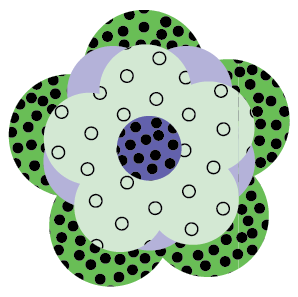
\includegraphics{doooodles_valborg-09.png}
	\end{center}
\end{wrapfigure}

Í þessum kafla verður farið yfir sanngildi,  \emph{samanburð} (e. comparison) og \emph{samanburðarvirkja} (e. comparison operators), \emph{rökvirkja} (e. logical operators) og svo \emph{skilyrðissetningar} (e. conditional statements).
Mikilvægt er að ná góðum tökum á þessum kafla ef halda á lengra inn í námsefnið, ef ekki er skilingur fyrir hendi á því hvernig segðir virka eða hvernig á að setja upp skilyrðissetningu er erfitt að ætla að halda mikið áfram.
Því er gott að gefa sér nægan tíma í þetta efni og gera ítarlegar tilraunir.

\section{Sanngildi}\index{Sanngildi}

Eins og kom fram í inngangi kaflans eru sanngildi einungis tvö, True og False.
Hægt er að geyma þau í breytum eins og gögn af öðrum týpum sem við höfum séð.
Sanngildi eru einnig metin sem 1 eða 0, fyrir True annars vegar og False hins vegar.

Vitandi að gildin geta verið 0 eða 1 (aldrei bæði í einu) er þess virði að nefna hérna sanntöflur.
Látum p vera yrðinguna ,,það er rigning“ og látum q vera yrðinguna ,,mér er kalt“.
Þá gætum við, með því að skoða mismunandi aðstæður, fengið rökrétt svar við spurningunum „er rigning og er mér kalt?“, sem við getum skrifað sem spurning1 (eða s1), og svo „er rigning eða er mér kalt?“, sem við getum kallað spurning2 (eða s2).

\begin{center}
%\centering
\begin{table}[h]
	\centering
\caption{Sanntafla}
\vspace{6pt}
\label{tbl:sanntafla}
\begin{tabular}{|c c|c|c|}
	% |c c|c| means that there are three columns in the table and% a vertical bar ’|’ will be printed on the left and right borders,
	% and between the second and the third columns.% The letter ’c’ means the value will be centered within the column,
	% letter ’l’, left-aligned, and ’r’, right-aligned.
	p & q & s1 & s2\\ 
	% Use & to separate the columns
	\hline  
	% Put a horizontal line between the table header and the rest.
	0 & 0 & 0 & 0\\
	0 & 1 & 0 & 1\\
	1 & 0 & 0 & 1\\
	1 & 1 & 1 & 1\\
	\end{tabular}

\end{table}
\end{center}

\begin{center}
	
\includegraphics[scale=0.65]{doooodles_valborg-14.png}
\end{center}

Ef við horfum á töflu \ref{tbl:sanntafla} sjáum við að yrðingarnar okkar um rigningu og kulda eru uppsettar þannig að hver lína í töflunni er einstakt ástand og allar mögulegar samsetningar koma fram.\footnote{Fjöldi lína í sanntöflu byggir á fjölda yrðinga sem á að skoða.
Ef það er bara ein yrðing þá er fjöldi lína 2, það er satt eða ósatt. Fjöldi lína er 2 í veldi fjölda staðhæfinga, í töflu \ref{tbl:sanntafla} eru yrðingarnar tvær og þá eru línurnar 2², og ef þær væru þrjár væri línufjöldinn 2³ og svo framvegis.}
Báðar yrðingar eru ósannar í fyrstu línunni, svo eru þær sannar sitt á hvað og í fjórðu línu eru þær báðar sannar.
Þá eru dálkarnir fyrir s1 og s2 svörin við spurningunum hér að ofan miðað við sanngildi yrðinganna í þeim tilteknu aðstæðum.
Í þeim aðstæðum þar sem er hvorki rigning né mér er kalt er svarið við báðum spurningum einnig neitandi (0).
Í þeim aðstæðum þar sem er bæði rigning og mér er kalt er svarið við báðum spurningum játandi (1).
Til þess að svarið við spurningu 1 sé játandi þarf mér því bæði að vera kalt og það þarf að vera rigning.
Svo þegar yrðingarnar eru ekki sannar á sama tíma skiptir ekki máli hvor er sönn því að önnur er ósönn og því er svarið neitandi.
Spurning 2 er hinsvegar orður þannig að það er nóg að annað hvort sé mér kalt eða það sé rigning úti til þess að svarið sé játandi.
Þannig er svarið alltaf játandi þegar yrðingarnar eru sannar á víxl.

\begin{lstlisting}[caption=Sanngildi geymd sem breytur, label=lst:bool-breytur]
satt = True
strengur = "True"
osatt = False
\end{lstlisting}

Akkúrat núna þurfum við bara að vita að týpan Boolean sé til og hvernig eigi að nota hana, með hástaf fremst.
Við sjáum svo í seinni köflum hvernig hún gagnast okkur.


\section{Segðir}\index{Segðir}

Eins og kom fram í inngangi kaflans má líta svo á að segðir séu sá hluti kóðans sem er metinn sem eitthvað gildi, eins og 4 + 5 er segð en x = 5 er yrðing.
Nú ætlum við þó að einblína á búlskar segðir, horfa á spurningar sem hafa svar sem er annað hvort satt eða ósatt.
Er rigning?
Þá horfum við út og sjáum að miðað við aðstæður er svarið annað hvort satt eða ósatt og það breytist eftir því hvenær við horfum.

\subsection{Samanburður}\index{Samanurður}
Hvað er samanburður?
Það er þegar eitthvað er metið miðað við eitthvað annað, eins og er þetta stærra en hitt?
Er þetta þyngra?
Er þetta jafngilt?
Athugið hér að aðalatriðið er að bera saman eitthvað tvennt, ekki er hægt að nota samanburð nema vera með tvennt í höndunum.
Þið hafið kannski lent á spjalli við barn sem segir ,,er ég stærri?“, stærri en hvað er ekki ljóst og við eigum því erfitt með að svara spurningunni.

Nú þurfum við nýtt hugtak, við erum búin að kynnast reiknivirkjum eins og + og - í kafla \ref{uk:tolur-reiknivirkjar}.
Nýja hugtakið okkar eru \textbf{samanburðarvirkjar}.
Samanburðarvirkjar eru notaðir til að spyrja hvort ákveðin tengsl gildi á milli einhverra tveggja hluta.
Þetta er eins og þegar við segjum í daglegu tali ,,er þetta epli stærra en þessi appelsína?“ þar með erum við að bera saman epli og appelsínur.
Samanburðarvirkjar eru til þess að gera slíka setningu formlega svo að tölva geti svarað spurningunni.

Samanburðarvirkjar eru nokkrir í Python:
\begin{itemize}
	\item[] \textbf{==} þá er spurt hvort hlutirnir sitthvoru megin við virkjann séu jafngildir.
	\item[] \textbf{!=} þá er spurt hvort hlutirnir sitthvoru megin við virkjann séu ólíkir.
	\item[] \textbf{<} þá er spurt hvort það sem er vinstra megin sé strangt minna en það sem hægra megin (3 er ekki minna en 3 t.d.).
	\item[] \textbf{>} þá er spurt hvort það sem er vinstra megin sé strangt stærra en það sem er hægra megin.
	\item[] \textbf{<=} þá er spurt hvort það sem er vinstra megin sé minna eða jafnt því sem er hægra megin.
	\item[] \textbf{>=} þá er spurt hvort það sem er vinstra megin sé stærra eða jafnt því sem er hægra megin.
\end{itemize}

Skoðum kóðabút þar sem þessir samanburðarvirkjar eru nýttir til þess annars vegar að fá niðurstöður með tölur og hins vegar strengi.
\begin{lstlisting}[caption=Samanburðarvirkjar, label=lst:bool-samanburður]
strengur1 = "abc"
strengur2 = "bcd"
strengur3 = "3"
tala1 = 3
tala2 = 3.0
tala3 = 4
print('jafngildissamanburður')
print(tala1 == tala3)
print(strengur1 == strengur2)
print(tala1 == tala2)
print(strengur3 == tala1)

print('minna en')
print(strengur1 < strengur2)

print('minna eða jafnt')
print(tala1 <= tala2)
\end{lstlisting}
\lstset{style=uttak}
\begin{lstlisting}
jafngildissamanburður
False
False
True
False
minna en
True
minna eða jafnt
True
\end{lstlisting}
\lstset{style=venjulegt}

Í kóðabút \ref{lst:bool-samanburður} er ekki verið að nota alla samanburðarvirkjana heldur einungis sýna hvernig er hægt að prófa sig áfram með þá.

\subsection{Rökvirkjar}\index{Rökvirkjar}
\textit{Rökvirkjar} (e. logical operators) í Python eru þrír, þeir eru \textbf{og}, \textbf{eða}  og \textbf{ekki} táknað með \texttt{and}, \texttt{or} og \texttt{not}.
Nöfn þeirra eru lykilorð í Python eins og nöfnin á týpunum sem við höfum séð (\textbf{str}, \textbf{int}, \textbf{float}, \textbf{list}) en rökvirkjar eru ekki gögn af einhverri týpu heldur eru meira eins og reiknivirkjarnir (+, -, *, **, //, \%).
Það sem þessir virkjar gera fyrir okkur er að taka tvær búlskar segðir og segja okkur eitthvað um samsetningu þeirra.
Tökum dæmi: ,,Kaffið er heitt og það eru til sítrónur“.
Hægt er að meta hvort kaffið sé heitt eða ekki og fá þannig út sanngildi fyrir þá segð eins og hægt er að gera fyrir segðina um sítrónurnar.
En tökum eftir að á milli þessara tveggja segða er rökvirkinn \textit{og}, sem segir okkur að til þess að meta gildi allrar setningarinnar þurfa báðar segðirnar sitthvorum megin við rökvirkjann að vera sannar til þess að setningin í heild sinni skili sönnu, annars er hún ósönn.
\vspace{10pt}
\begin{itemize}
	\item[] \textbf{and} til þess að segð með þessum rökvirkja sé sönn þurfa báðar hliðar að vera sannar, annars er hún ósönn
	\begin{itemize}
		\item Það má líta á \textit{og} rökvirkjann eins og margföldun, hann hefur forgang umfram \underline{eða}.
		\item Þar sem satt er 1 og ósatt 0 fáum við alltaf út 0 ef við margföldum með 0.
		\item ,,það er heitt úti“ og ,,það er kalt úti“ myndi skila okkur ósönnu því ekki getur bæði verið satt.
		\item ,,það er heitt úti“ og ,,klukkan er fimm“ myndi skila okkur sönnu eftir aðstæðum.
	\end{itemize}
	\item[] \textbf{or} til þess að segð með þessum rökvirkja sé sönn þarf önnur hvor hliðin að vera sönn, annars er hún ósönn.
	\begin{itemize}
		\item Það má líta á \textit{eða} rökvirkjann eins og samlagningu.
		\item Þar sem satt er 1 og ósatt 0 þurfum við bara að sjá 1 einu sinni til þess að útkoman í heild sinni verði sönn.
		\item ,,það er heitt úti“ eða ,,það er kalt úti“ myndi skila okkur sönnu ef þetta væru þau einu tvö hitastig sem væru í boði.
		\item ,,það er heitt úti“ eða ,,klukkan er fimm“ myndi skila sönnu eftir aðstæðum.
	\end{itemize}
	\item[] \textbf{not} snýr við sanngildi segðar, not er ekki sett á milli segða heldur fyrir framan eina segð.
	\begin{itemize}
		\item Það má líta á rökvirkjann \textit{ekki} eins og mínus, hann snýr við sanngildi eins og formerki.
		\item Ekki satt yrði ósatt, ekki ósatt yrði satt.
		\item neitum með \texttt{ekki} á yrðinguna ,,það er heitt úti“ skilaði yrðingunni ,,það er ekki heitt úti“.
	\end{itemize}
\end{itemize}

\vspace{5pt}
\begin{itarefni}
\textbf{Rökvirkjar sem reikniaðgerðir}\\
Til að halda áfram með þessa samlíkingu með margföldun, samlagningu og mínus skulum við skoða eftirfarandi reikningsdæmi:
1$\cdot$1$\cdot$1$\cdot$0 + 1$\cdot$0 + (-1).
Hér gerum við ráð fyrir að hver hluti af þessu reikningsdæmi sé yrðing sem búið er að meta sem sanna eða ósanna eftir þeim aðstæðum sem við erum í (kaffið er heitt, það er kalt úti og þess háttar).
Þegar við reiknum þetta dæmi sjáum við að margfaldað er með 0 í báðum þáttunum þar sem margföldun kemur fyrir svo útkoman í báðum verður núll.
Þessi síðasti liður er okkur ekki eins eðlislægur en við munum að það eru bara til 0 eða 1 og mínus skiptir gildinu okkar svo við hljótum að enda með 0.
Við endum því í 0 + 0 + 0 sem gefur okkur 0 og því er öll segðin metin sem ósönn.
\end{itarefni}


\section{Skilyrðissetningar}\index{Skilyrðissetningar}
Nú viljum við vita til hvers í ósköpunum við vorum eiginlega að leggja það á okkur að skilja hvenær eitthvað er satt eða ósatt.
Það er einmitt heilmikið tölvunarfræðilegt gagn í því að geta spurt svona já eða nei spurninga sem tölvan getur svarað.
Til dæmis viljum við geta framkvæmt einhverja aðgerð í forritinu okkar \textbf{ef} einhver skilyrði eru fyrir hendi.
Segjum að við séum með vekjaraklukku sem við forritum til að hringja þegar klukkan er orðin 8.
Þá viljum við geta spurt tölvuna hvort að það sé satt eða ósatt að klukkan sé orðin 8.

Ef klukkan er ekki orðin 8 viljum við ekki gera neitt, en ef hún er orðin átta þá viljum við að hún spili einhvern hljóm eða titri.
Við gætum líka verið að forrita einfaldan tölvuleik eins og hengimann, ef spilarinn er ekki búinn að giska á alla stafina í orðinu okkar viljum við geta beðið viðkomandi að spyrja aftur.
\textbf{Annars} viljum við að notandinn fái verðlaun fyrir að hafa giskað á rétt orð.\footnote{Hérna er gert ráð fyrir að mega giska óendanlega oft rangt.}
Einnig gætum við viljað gera eitthvað ákveðið þá og því aðeins að eitthvað annað var ósatt.
Ef við notum okkar eigin máltilfinningu til að leggja skilning í eftirfarandi setningu: ,,Ef við eigum ekki mjólk vil ég kaupa mjólk, ef svo er ekki vil ég athuga hvort að við eigum kex og ef við eigum ekki kex vil ég kaupa það, annars fer ég ekkert í búðina.“
Hér er aðaláherslan lögð á mjólkurstöðuna okkar, ef við eigum ekki mjólk viljum við laga það, en ef við eigum mjólk þá getum við gert eitthvað annað.

Þarna eru komnar aðstæður þar sem við athugum mjólkurstöðuna og fyllum á ef þarf, en ef við eigum nóg af mjólk viljum við samt athuga hvort við eigum nóg af kexi því að við gætum þurft að fylla á þar.
Þetta er kannski ekki augljóst en ef það vantar mjólk skiptir ekki máli hvort það vanti kex eða ekki, við förum í búðina og kaupum mjólk, við kaupum ekki kex.
Þetta skilst kannski frekar á flæðiriti sem sést á mynd \ref{fig:flæðirit}.
Flæðiritið líkir eftir uppsetningu á skilyrðissetningum þannig að það sem er inni í grænum þríhyrningum eru spurningar sem þarf að svara, bláu ferhyrningarnir eru svo niðurstöður sem fást í málið.

\tikzstyle{startstop} = [rectangle, rounded corners, minimum width=3cm, minimum height=1cm,text centered, draw=black, fill=red!30]
\tikzstyle{io} = [trapezium, trapezium left angle=70, trapezium right angle=110, minimum width=2cm, minimum height=1cm, text centered, draw=black, fill=blue!30]
\tikzstyle{process} = [rectangle, minimum width=3cm, minimum height=1cm, text centered, draw=black, fill=laurapurple!40]
\tikzstyle{decision} = [diamond, minimum width=3cm, minimum height=3cm, text centered, draw=black, fill=ocre!60]
\tikzstyle{arrow} = [thick,->,>=stealth]

\vspace{5pt}
\begin{figure}[H]
	\centering
\begin{tikzpicture}[node distance=2cm]

\node (mjolk) [decision] {Engin mjólk};
\node (s0) [left of=mjolk, xshift=-3cm] {};
\node (kex) [decision, below of=mjolk, yshift=-1.5cm] {Ekkert kex};
\node (bud1) [process, right of=mjolk, xshift=3cm] {Kaupa mjólk};
\node (bud2) [process, right of=kex, xshift=3cm] {Kaupa kex};
\node (bud3) [process, below of=kex, yshift=-0.5cm] {Vera heima};
\draw [arrow] (s0) -- node[anchor=south] {byrja} (mjolk);
\draw [arrow] (mjolk) -- node[anchor=west] {ósatt} (kex);
\draw [arrow] (mjolk) -- node[anchor=south] {satt} (bud1);
\draw [arrow] (kex) -- node[anchor=south] {satt} (bud2);
\draw [arrow] (kex) -- node[anchor=west] {ósatt} (bud3);
\end{tikzpicture}
\caption{Hér sést eftirfarandi setningin í flæðiriti: ,,Ef við eigum ekki mjólk vil ég kaupa mjólk, ef svo er ekki vil ég athuga hvort við eigum kex og ef við eigum ekki kex vil ég kaupa það, annars fer ég ekkert í búðina“. Ef það er engin mjólk förum við og kaupum mjólk, en ef það er til mjólk þá athugum við hvort að það sé til kex og kaupum það ef það vantar.
Ef við hins vegar eigum bæði kex og mjólk er engin ástæða til að fara í búðina.}
\label{fig:flæðirit}
\end{figure}
\todo{formatting}
\vspace{5pt}

Vegna þess að áherslan er lögð á ,,við eigum ekki mjólk“ er vitlegast að setja inn segð sem er með neitun.
Ef yrðingin m stendur fyrir setninguna ,,við eigum mjólk“ er yrðingin ekki m (not m) ,,við eigum ekki mjólk“.
Skoðum þetta í töflu \ref{tbl:sanntafla-kaffi}, sambærilegri þeirri sem við sáum áður (tafla \ref{tbl:sanntafla}), nema í staðinn fyrir p og q notum við yrðinguna ,,það er til mjólk“.

Ef þessu væri skellt í eina spurningu með rökvirkjanum \emph{og} yrði spurningin ,,er engin mjólk og ekkert kex til?“
Ef henni yrði svo svarað neitandi vitum við ekki hvort það var út af mjólkinni eða kexinu.
Það gæti þó verið að það skipti ekki máli og því nauðsynlegt að geta beitt rökvirkjunum á hagnýtan máta.

\begin{center}
	\centering
	\begin{table}[H]
		\centering
		\caption{Sanntafla með ákveðnum yrðingum}
		\vspace{3pt}
		\label{tbl:sanntafla-kaffi}
		\begin{tabular}{|c | c| c |}
			% |c c|c| means that there are three columns in the table and% a vertical bar ’|’ will be printed on the left and right borders,
			% and between the second and the third columns.% The letter ’c’ means the value will be centered within the column,
			% letter ’l’, left-aligned, and ’r’, right-aligned.
			m = það er til mjólk & ekki m = það er ekki til mjólk\\ 
			% Use & to separate the columns
			\hline  
			% Put a horizontal line between the table header and the rest.
			0 & 0 & Bæði ósatt, getur ekki verið\\
			0 & 1 &\\
			1 & 0 &\\
			1 & 1 & Bæði satt á sama tíma, getur ekki verið\\
			\hline
		\end{tabular}
		
	\end{table}
\end{center}
Við viljum að aðalatriðið komi fram í inngangspunktinum í skilyrðissetningunni okkar til að hún sé skýrt upp sett og skiljanleg, til þess gætum við þurft að nota neitun.
Við sjáum betur í næstu þremur undirköflum hvað ætti að fara á hvaða stað, en eins og með góðar nafnavenjur þegar við nefnum breyturnar okkar skulum við venja okkur á það strax í upphafi að hafa skilyrðissetningarnar okkar skýrar.

Nú höfum við séð í inngangi þessa undirkafla orðunum ef og annars slengt fram.
Við þekkjum þessi orð og skiljum hvernig á að nota þau í setningu til að kalla fram útkomu.
En það sem við þurfum að gera núna er að átta okkur á því að þessi orð eru mun formlegri í forritun heldur en í daglegu tali.
Sem dæmi má taka setninguna: ,,Ertu ekki að hugsa um Jamie Lee Curtis?“
Í íslensku er hægt að svara þessari spurningu með ,,já ég er ekki að hugsa um hana“ eða ,,nei ég er ekki að hugsa um hana“ og bæði skilst.
Einnig er hægt að segja ,,jú ég er að hugsa um hana“.
Forritunarmál eru ekki tungumál, þau eru formleg og því er engin tvíræðni í boði.

Skoðum því nú hvað það þýðir að nota \textit{skilyrðissetningar} (e. conditional statements) í Python með lykilorðunum \textbf{if - elif - else}, sem verða þó tekin fyrir annarri röð, vegna þess best er að útskýra elif síðast þar sem það er búið til úr else og if.

\subsection{if}\index{if}
Fyrsta lykilorðið sem við tökum fyrir er \textbf{if}, þar sem ekki er hægt að búa til skilyrðissetningu án þess.
Og nú þurfum við að huga að því hvernig kóðinn okkar er uppsettur.
Það sem á að framkvæma undir ef setningunni/if yrðingunni er inndregið um fjögur bil eða einu sinni á tab takkann.
Eina sem ræður því hvað fer mikið af kóða undir hverja yrðingu er hóf og skynsemi.
Við sjáum svo í kafla \ref{uk:hreiðrun} um hreiðrun hvers vegna það er mikilvægt að skilyrðissetningar séu skýrar.
\begin{wrapfigure}{o}{0.2\textwidth} %i o r l 
	\begin{center}
		
\includegraphics{doooodles_valborg-15.png}
	\end{center}
\end{wrapfigure}
Góð venja er að búa til skilyrðissetningar þar sem aðalvirknin á sér stað inni í if yrðingunni, þannig að segðin sem fer þar inn passi við það sem eigi að framkvæma.
Tökum aftur dæmið um mjólkina og búðarferðina í mynd \ref{fig:flæðirit} og skoðum hvernig flæðiritið breytist eftir því hvernig við orðum skilyrðin.
Skoðum þar hvernig uppsetningin á flæðiritinu verður bjöguð ef við orðum spurninguna með játun en ekki neitun: ,,Ef það er til mjólk vil ég athuga hvort það sé til kex ef svo er vil ég vera heima, annars kaupi ég kex, ef það er til mjólk en ekki kex og annars kaupi ég mjólk ef það er ekki til mjólk.“
Þetta er kannski ekki nógu flókin setning til þess að valda þeim hughrifum sem ætlast er til, en við sjáum að til þess að komast að þeim endapunkti sem aðaláherslan er á, ,,vera heima“ þar sem hún er fyrsti endapunkturinn okkar, þurfum við að fara í gegnum tvær spurningar.
Með því að orða spurninguna öðruvísi erum við búin að setja upp skilyrðissetninguna þannig að mjólkurstaðan er núna ekki lengur í forgrunni, við virðumst frekar vera að reyna að halda okkur heima.

\begin{figure}[H]
	\centering
	\begin{tikzpicture}[node distance=2cm]
	\node (mjolk) [decision] {Mjólk er til};
	\node (s0) [left of=mjolk, xshift=-3cm] {};
	\node (kex) [decision, right of=mjolk, xshift=2cm] {Kex er til};
	\node (bud1) [process, below of=mjolk, yshift=-2cm] {Kaupa mjólk};
	\node (bud2) [process, below of=kex, yshift=-2cm] {Kaupa kex};
	\node (bud3) [process, right of=kex, xshift=2cm] {Vera heima};
	\draw [arrow] (s0) -- node[anchor=south] {byrja} (mjolk);
	\draw [arrow] (mjolk) -- node[anchor=south] {satt} (kex);
	\draw [arrow] (mjolk) -- node[anchor=west] {ósatt} (bud1);
	\draw [arrow] (kex) -- node[anchor=west] {ósatt} (bud2);
	\draw [arrow] (kex) -- node[anchor=south] {satt} (bud3);
	\end{tikzpicture}
	\caption{Hér sést eftirfarandi setning í flæðiriti: ,,Ef það er til mjólk vil ég athuga hvort það sé til kex, ef svo er vil ég vera heima, annars kaupi ég kex ef það er til mjólk en ekki kex og annars kaupi ég mjólk ef það er ekki til mjólk.“
	Þetta veldur því að aðaláherslan virðist nú vera að komast að því hvort eigi að kaupa kex eða vera heima og mjólkurstaðan er athuguð fyrst af einhverri ástæðu.
	Setningin í heild er frekar ruglingsleg og hún kom mun betur út í flæðiritinu á mynd \ref{fig:flæðirit}.
	Þó áherslan sé önnur er niðurstaðan sú sama, það er á ábyrgð forritara að skrifa kóða sem er læsilegur og skiljanlegur.}
	\label{fig:flæðirit-neitun}
\end{figure}

Skoðum nú kóðabút \ref{lst:if} og hvað er átt við með réttum inndrætti, hér er if setning sýnd ein og stök.
Í kóðabútnum tökum við fyrir segðina ,,er til mjólk?“ og veitum henni gildið \texttt{True} þannig að við erum stödd í þeim aðstæðum að við eigum vissulega til mjólk, skoðið töflu \ref{tbl:sanntafla-kaffi} til að sannfærast um það sem er að gerast.
Við sjáum í næsta undirkafla hvað við getum gert ef við förum framhjá if setningunni okkar og viljum gera eitthvað í því tilfelli.
Akkúrat núna getum við spurt ,,er rigning?“ og ef svo er gert eitthvað í því, eins og að prenta út einhvern streng.
Þannig keyrum við kóðann í línu 4 einungis ef við komumst þangað inn, en við kæmumst fram hjá (eins og það var orðað hér framar) ef segðin skilaði ekki sanngildi í línu 3.

\begin{lstlisting}[caption=if notað, label=lst:if]
mjolk = True 

if(mjolk):
	print('við fórum í búðina og keyptum mjólk')
\end{lstlisting}
\lstset{style=uttak}
\begin{lstlisting}
# við áttum mjólk svo ekkert prentast
\end{lstlisting}
\lstset{style=venjulegt}

\subsection{else}\index{else}
Lykilorðið \textbf{else} má fylgja \textbf{if}, en það er ekki nauðsynlegt.
Hins vegar verður að vera eitthvað \emph{ef} til þess að það geti verið eitthvað \emph{annars}.
Setningin ,,annars kaupi ég mjólk“ er ekki sérlega vitræn því að okkur vantar alveg fyrri hlutann.
Einnig er ekki mjög gáfulegt að segja ,,ég kaupi mjólk ef vantar annars kaupi ég kex annars kaupi ég te annars...“.
Því er einungis hægt að setja eitt annars við hvert ef, sjáum kóðabút \ref{lst:else}.
Sú klausa keyrist einungis þegar ef setningin sem hún hangir fyrir neðan keyrist ekki, það er eina skilyrðið.
Það þarf ekki að spyrja neinnar spurningar sem er metin sem boolean gildi til að keyra else, það mun alltaf keyrast þegar segðin í ef yrðingunni er ósönn.

\begin{lstlisting}[caption=else notað, label=lst:else]
mjolk = True

if(not mjolk):
	print('við fórum í búðina og keyptum mjólk')
else:
	print('vera heima')

if(3 < 4):
	print("þrír er minna en fjórir")
else:
	print('ég fer ekki hingað inn, því 3 er vissulega minna en fjórir, en það er gott að vera við öllu búin')
\end{lstlisting}
\lstset{style=uttak}
\begin{lstlisting}
vera heima
þrír er minna en fjórir
\end{lstlisting}
\lstset{style=venjulegt}

Mikilvægt er að geta sett svona annars-klausu því við viljum geta brugðist við ef upphaflega skilyrðið okkar er ósatt.
Við viljum geta tekið á fleiri tilfellum en bara upphafsskilyrðinu okkar.

%\begin{wrapfigure}{o}{0.2\textwidth} %i o r l 
\begin{center}
	
\includegraphics[scale=2]{doodles31-27.png}
\end{center}
%\end{wrapfigure}


\subsection{elif}\index{elif}
En hvað ef við viljum geta tekið á einhverju sérstöku tilfelli, sem kemur einungis upp í ákveðnum aðstæðum?
Við viljum ekki bara grípa það að inngangspunkturinn okkar hafi verið ósannur heldur viljum við einnig skoða eitthvað fleira.
Þarna kemur setningin um mjólkina, kexið og búðarferðirnar aftur inn.
Þá getum við sagt ,,ef það er ekki til mjólk fer ég í búð, \textbf{annars ef} það er ekki til kex fer ég í búð og kaupi kex, nú annars er engin ástæða til að fara í búðina og ég verð bara heima“.
Við viljum bara nota þetta seinna ef í ákveðnu tilfelli, við höfum ekkert að gera við kexið ef það er engin mjólk svo það er aðeins keyrt ef við eigum hana.
Við sjáum þetta forritað í kóðabút \ref{lst:elif}.

Skilyrðissetningar eru settar upp þannig að það verður að vera eitt \textbf{if}, svo mega koma núll eða fleiri \textbf{elif} og að lokum má setja 0 eða 1 \textbf{else}.
Þetta er eins og málfræðilegur skilningur okkar er á tungumálinu, við megum hengja endalaust af annars ef klausum inn í setningarnar okkar, það verður þá bara erfiðara að skilja þær (kóðann sömuleiðis).
\begin{figure}[H]
	\centering
	\begin{tikzpicture}[node distance=1cm]

		
		
		\node (ef) [decision, minimum height = 2.0cm, minimum width = 2.0cm] {ef};
		\node (s0) [left of=ef, xshift=-2cm] {};
		\node (annars1) [decision, minimum height = 1cm,minimum width = 1cm, 
		right of=ef, xshift=2cm, yshift = -2cm] {annars ef};
		\node (annars2) [decision, minimum height = 1cm,minimum width = 1cm, 
		right of=annars1, xshift= 2cm, yshift=-2cm] {...};
		\node (annars3) [decision, minimum height = 1cm,minimum width = 1cm, 
		right of=annars2, xshift= 2cm, yshift=-2cm] {annars ef};
		\node (annars) [process, minimum height = 1cm,minimum width = 1cm, 
		right of=annars3, xshift=2cm, yshift=-2cm] {annars};
		\node (efs) [below of= ef, yshift = -2.5cm] {};
		\node (annars1s) [below of= annars1, yshift = -2cm] {};
		\node (annars2s) [below of= annars2, yshift = -2cm] {};
		\node (annars3s) [below of= annars3, yshift = -2cm] {};
		\node (annarss) [below of= annars, yshift = -1cm] {};
		\draw [arrow] (s0) -- node[anchor=south] {byrja} (ef);
		\draw [arrow] (ef) -| node[anchor=south] {ósatt} (annars1);
		\draw [arrow, dashed] (annars1) -| node[anchor=south] {} (annars2);
		\draw [arrow, dashed] (annars2) -| node[anchor=south] {} (annars3);
		\draw [arrow] (annars3) -| node[anchor=south] {ósatt} (annars);
		\draw [arrow] (ef) -- node[anchor=west] {satt} (efs);
		\draw [arrow] (annars1) -- node[anchor=west] {satt} (annars1s);
		
		\draw [arrow] (annars2) -- node[anchor=west] {} (annars2s);
		
		\draw [arrow] (annars3) -- node[anchor=west] {satt} (annars3s);
		
		\draw [arrow] (annars) -- node[anchor=west] {} (annarss);
	\end{tikzpicture}
	\caption{Hér sjáum við flæðirit yfir virkni skilyrðissetninga.
		Það verður að vera ein \textbf{if} setning fremst, svo mega koma eins margar \textbf{elif} setningar þar fyrir neðan eins og við viljum og að lokum má koma nákvæmlega ein \textbf{else} klausa.}
	\label{fig:flæðirit-skilyrði}
\end{figure}

\begin{lstlisting}[caption=elif notað, label=lst:elif]
mjolk = True 
kex = False 

if(not m):
	print('við fórum í búðina og keyptum mjólk')
elif(not k):
	print('við fórum í búðina og keyptum kex')
else:
	print('vera heima')

if(5 < 4):
	print("fimm er minna en fjórir")
elif(4 < 4):
	print("fjórir er minna en fjórir!")
elif(3 < 4):
	print("þrír er minna en fjórir")
elif(2 < 4):
	print("en 2 er líka minna en fjórir!")
else:
	print('eitthvað er að')
\end{lstlisting}
\lstset{style=uttak}
\begin{lstlisting}
við fórum í búðina og keyptum kex
þrír er minna en fjórir
\end{lstlisting}
\lstset{style=venjulegt}


\subsection{Hreiðrun}\index{Hreiðrun}\label{uk:hreiðrun}
\emph{Hreiðrun} (e. nesting) þýðir að setja eitthvað endurtekið undir eitthvað annað, eins og babúska dúkkur eða þegar gjöf er pakkað inn í mörg lög af gjafapappír.
Í forritun þýðir hreiðrun að yrðing af einhverri tegund tilheyri og sé keyrð innan í yrðingu af sömu tegund.
Við getum hugsað þetta í samhengi við skilyrðissetningar, að við séum með innri skilyrðissetningar sem þarf einnig að meta til þess að komast að niðurstöðu.
Skoðum þetta aftur í samhengi við mjólkurkaupin nema nú bætum við því við að við eigum bara ákveðið mikinn pening, sjá kóðabút \ref{lst:nesting}.

\begin{lstlisting}[caption=Hreiðrun, label=lst:nesting]
mjolk = True 
kex = False 
peningar = 100 

if(not mjolk):
	if(p > 200):
		print('við fórum í búðina og keyptum mjólk því við vorum með nógu mikinn pening')
	else:
		print('okkur vantaði mjólk en við vorum ekki með nógu mikinn pening')
elif(not kex):
	if(p > 99):
		print('við fórum í búðina og keyptum kex því við vorum með nægan pening')
	else:
		print('okkur vantaði kex en við vorum ekki með nægan pening')
else:
	print('vera heima og geyma allan peninginn')
\end{lstlisting}
\lstset{style=uttak}
\begin{lstlisting}
við fórum í búðina og keyptum kex því við vorum með nægan pening
\end{lstlisting}
\lstset{style=venjulegt}

Hreiðrun er gagnleg þegar við viljum skoða ákveðið innra skilyrði aðeins ef ytra skilyrðinu er mætt.
Skoðið núna aftur myndir \ref{fig:flæðirit} og \ref{fig:flæðirit-neitun} og sjáið hvernig mætti beita hreiðrun eða annars-ef setningu til þess að forrita hugmyndina á bakvið vandamálið.

\section{Inntak}\index{Inntak}
\begin{wrapfigure}{i}{0.4\textwidth} %i o r l 
	\begin{center}
		
\includegraphics[scale=2]{doooodles_valborg-08.png}
	\end{center}
\end{wrapfigure}
Nú höfum við verið að skoða spurningar og svör við þeim sem við skráðum sjálf.
Það sem við viljum geta gert er að spyrja notandann að einhverju og geta gert eitthvað byggt á því svari.
Við þurfum að fá \emph{inntak} (e. input) frá notandanum.
Þá lærum við um nýtt innbyggt fall í Python sem heitir \texttt{input()}.
Það sem fallið gerir er að taka við streng frá notanda, notandi skrifar eitthvað inn í þar til gert svæði og við getum notað það í forritinu okkar.\footnote{Notkun \texttt{input()} í skipanalínu gefur okkur nýja línu til að svara.
	Jupyter Notebooks gefur okkur lítinn glugga til að skrifa svarið okkar í fyrir neðan selluna þar sem \texttt{input()} skipunin er keyrð.}

Skoðum kóðadæmi í kóðabút \ref{lst:input}, þar sem við geymum svarið frá notanda í breytunni \texttt{svar} og viðfangið sem við settum inn í input fallið er strengur sem inniheldur spurninguna sem notandinn sér.
Þar sést þó ekki þegar inntaksglugginn var notaður.

Fallið \texttt{input()} skilar okkur alltaf streng.
Ef við viljum geta spurt notandann um tölustafi þurfum við að kunna að kasta á milli gagnataga sjálf og við sjáum hvernig það er gert í kóðabút \ref{lst:kast}


\begin{lstlisting}[caption=input() fallið notað, label=lst:input]
svar = input('skrifaðu nafnið þitt')
print('halló', svar)
\end{lstlisting}
\lstset{style=uttak}
\begin{lstlisting}
 Valborg
halló Valborg
\end{lstlisting}
\lstset{style=venjulegt}

Mikilvægt er að skilja og nota \texttt{input()} á þessu stigi málsins, því að við verðum að átta okkur á því að þegar við forritum erum við miklu meira að vinna með breytunöfn heldur en gögn sem við getum horft á.
Í kóðabút \ref{lst:input} kemur hvergi fram í kóðanum að nafnið sé Valborg og það getur verið hvað sem er, við prentum bara út það sem notandinn gaf okkur án þess að vera eitthvað að skoða hvað það er.
Oft vilja byrjendur horfa á gögnin sín og setja inn niðurstöður fyrir tölvuna, til dæmis endar verkefnið ,,búðu til breytu sem inniheldur nafn og prentaðu út breytuna ásamt strengnum 'halló:'“ endar í kóða eins og sést í kóðabút \ref{lst:byrjendur}.
Annað verkefni væri að finna miðju í streng sem hægt er að gera með \texttt{len(strengur)//2}, en byrjendum finnst eðlislægara að finna lengdina, finna svo helminginn af því og nota svo loks þá tölu

\begin{lstlisting}[caption=Oft forðast byrjendur að nota breytur og treysta meira á að sjá hvað ætti að koma út, label=lst:byrjendur]
nafn = 'Valborg'
print('Halló: Valborg')

strengur = "þessi strengur hefur 31 tákn!!!"
# þetta þyrfti að gera í skrefum
print(len(strengur)) 
print(31/2) 
print(strengur[15])

print(strengur[len(strengur)//2])
\end{lstlisting}
\lstset{style=uttak}
\begin{lstlisting}
Halló: Valborg
31
15.5
h
h
\end{lstlisting}
\lstset{style=venjulegt}

Í kóðabút \ref{lst:byrjendur} sést að fyrst þarf að keyra línuna \texttt{len(strengur)} til þess að komast að því að setja vísi 15 inn.
Svo þarf að deila þeirri tölu með tveimur til að finna miðjuna og síðan þarf handvirkt að setja þá tölu inn eftir að hafa breytt henni í næstu heilu tölu.
Það sem er að gerast er ekkert rangt, það er hins vegar mikil vannýting á því sem tölvan getur gert fyrir okkur.
Þetta eykur vinnuna fyrir okkur sjálf umtalsvert því að það þarf að keyra hvert skref í kóðabútnum fyrir sig til að komast að því hvað eigi að gera í næsta skrefi, í stað þess að gera það í einni línu eins og í línu 10.

\subsection{Kastað á milli gagnataga}
Til þess að geta unnið með gögn eins og þá týpu sem við viljum þurfum við að læra að \emph{kasta} á milli taga/týpna (e. typecasting).
Þetta þýðir að við látum vélina umrita gögnin okkar yfir í annað gagnatag, sem er einungis hægt ef gögnin eru sambærileg týpunni sem á að kasta í.

Þá koma lykilorðin sem við höfum lært fyrir týpurnar okkar að gagni.
Við þekkjum núna strengi með lykilorðið \textbf{str}, heiltölur með lykilorðið \textbf{int}, fleytitölur með lykilorðið \textbf{float} og lista með lykilorðið \textbf{list}.
Þá notum við lykilorðið eins og fall og setjum inn í fallið sem viðfang það sem á að verða að því gagnatagi sem lykilorðið segir til um.
Við sjáum í kóðabút \ref{lst:kast} hvernig á að fara að þessu.

Nú höfum við séð að \texttt{input()} fallið skilar alltaf til okkur gögnum af taginu/týpunni strengur.
Við viljum kannski geta unnið með inntakið frá notandanum sem tölu.
Ef strengurinn inniheldur einungis tölur á bilinu 0-9 er hægt að geyma hann sem heiltölu eða fleytitölu, en ef hann inniheldur einungis tölur á bilinu 0-9 og nákvæmlega einn punkt er hægt að geyma hann sem fleytitölu.


\begin{lstlisting}[caption=Hvernig á að kasta á milli gagnataga, label=lst:kast]
talnastrengur = "123"
heiltala = int(talnastrengur)
fleytitala = float(talnastrengur)

fleytitolustrengur = "3.1415"
talan_pi = float(fleytitolustrengur)
\end{lstlisting}

Nú þegar við vitum að við getum fengið streng í hendurnar frá notanda, vitandi það að við báðum um tölu, getum við leyft okkur að kasta strengnum í það talnatag sem okkur hentar.
\begin{wrapfigure}{i}{0.2\textwidth} %i o r l 
	\begin{center}
		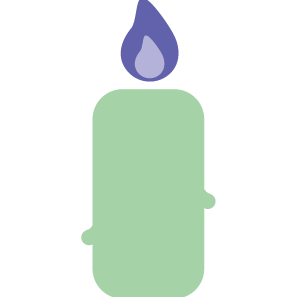
\includegraphics{doooodles_valborg-13.png}
	\end{center}
\end{wrapfigure}
Við sjáum svo í seinni hluta bókarinnar hvernig á að taka á mismunandi tilfellum og reyna á eitthvað sem gæti valdið villu án þess að það skemmi fyrir okkur.
Núna ætlum við að láta sem við getum treyst notendum til að gefa okkur inntak sem samræmist því sem við báðum um.
Prófið ykkur nú áfram með að kasta á milli taga, þið munið fá einhverjar villur og það er frábært.
Gerið tilraunir og prófanir, kastið á milli allra þeirra taga sem þið þekkið í öll þau tög sem þið þekkið, hvað má og hvað má ekki?

Við viljum kasta á milli taga til þess að geta beitt þeim aðgerðum og aðferðum sem eru í boði fyrir það gagnatag sem við sækjumst eftir að nota.
Til dæmis er ekki hægt að sækja þriðja tölustafinn í heiltölu en ef við köstum henni í streng getum við sótt táknið í sætisnúmeri 2 og fengið þannig þriðja tölustafinn.

\begin{itarefni}
\textbf{Dæmi um notkun á kasti milli taga}\\
Seinna munum við sjá gagnatýpuna mengi.
Ein gagnleg notkun á kasti milli taga væri að kasta lista í mengi til að losna við tvítekningar og kasta menginu svo í lista aftur.\\
\texttt{a = [1, 2, 2]}\\
\texttt{b = set(a)}\\
\texttt{a = list(b)}\\
Nú er listinn \texttt{a} orðinn að \texttt{[1,2]}, sjá meira um það í kafla \ref{k:sett}.
\end{itarefni}


%--------------------------------Æfingar------------------------%


\newpage
\section{Æfingar}
\begin{exercise}\label{exp1}
Búið til tvær talnabreytur, látið svo skilyrðissetningu prenta út þá sem er stærri.
\end{exercise}
\setboolean{firstanswerofthechapter}{true}
\begin{Answer}[ref={exp1}]
Byrjum á svari, förum svo í réttara svar og svo loks ekki rétt svar.

Við erum beðin um skilyrðissetningu svo við þurfum \texttt{if}.
\begin{lstlisting}
a = 3
b = 4
if(a > b):
	print(a)
else:
	print(b)\end{lstlisting}

Hér tökum við ekki á því tilviki að \texttt{a} og \texttt{b} séu jafnstór, sem gæti verið mikilvægt að hunsa ekki.
Við lögum þetta til, miðað við aðstæður (þessi lausn gæti verið óhentug þegar við förum að skoða skilagildi í kafla \ref{k:föll}).
\begin{lstlisting}
a = 3
b = 4
if(a > b):
	print(a)
elif(b > a):
	print(b)
else:
	print('breyturnar eru jafnstórar')\end{lstlisting}

	
Hér ætlum við að svo að skoða eina nálgun sem skilar okkur ekki réttri lausn, því við erum beðin um að prenta út þá breytu sem er stærri en ekki finna út hvort fyrri sé stærri en hin.
\begin{lstlisting}
a = 3
b = 4
print(a > b)\end{lstlisting}
Þetta skilar okkur svarinu \texttt{False} því að \texttt{a} er vissulega ekki stærra en \texttt{b} en þarna er samanburður, er það ekki nóg?
Nei, ekki alveg, skilyrðissetning er með \texttt{if}, þarna erum við með segð.
\end{Answer}
\setboolean{firstanswerofthechapter}{false}

\begin{exercise}\label{exp2}
Búið til tvær breytur sem innihalda báðar sanngildi (True eða False), að eigin vali.
Skrifið svo segð þar sem spurt er: fyrri breytan eða ekki seinni breytan?
\end{exercise}
\begin{Answer}[ref={exp2}]
Hér erum við að æfa okkur að nota rökvirkja, við eigum að nota \texttt{or} og \texttt{not}.
	\begin{lstlisting}
fyrri = False
seinni = True
print(fyrri or not seinni)\end{lstlisting}
\end{Answer}

\begin{exercise}\label{exp3}
Búið til þrjár talnabreytur og skrifið svo segð sem spyr eftirfarandi spurningar um þær breytur: eru breytur 1 og 2 jafngildar og er breyta 2 lægri en breyta 3 eða er breyta 1 stærri en breyta 3?
\end{exercise}
\begin{Answer}[ref={exp3}]
	Hér erum við að æfa okkur að nota rökvirkja og samanburðarvirkja, við eigum að nota \texttt{or}, \texttt{and}, \texttt{==}, \texttt{<}, \texttt{>} í þessari segð.
	\begin{lstlisting}
eitt = 1
tvo = 1
thrju = 1
print(eitt == tvo and tvo < thrju or eitt > thrju)\end{lstlisting}
\end{Answer}

\begin{exercise}\label{exp4}
Nú skulum við búa til þrjár breytur sem eru hliðar í þríhyrningi.
Þríhyrningar geta verið margs konar en við ætlum að einbeita okkur að tveimur tegundum, jafnhliða (allar hliðar jafnlangar) og jafnarma (tvær hliðar jafnlangar).

Nú ætlið þið að skrifa forritsbút þar sem eru þrjár talnabreytur fyrir hliðarnar þjár á einhverjum þríhyrningi og forritið ykkar prentar út, með skilyrðissetningu, hvort að þríhyrningurinn sé jafnhliða, jafnarma eða hvorugt.

Prófið svo að keyra aftur fyrir aðrar tölur þannig að þið sannfærist um að kóðinn sé réttur.
\end{exercise}
\begin{Answer}[ref={exp4}]
Setjum hliðarnar sem \texttt{a}, \texttt{b}, og \texttt{c}.
Til þess að kóðinn sé réttur þurfa tölurnar 1, 3, 1 að skila 'jafnarma', tölurnar 2, 2, 2 þurfa að skila 'jafnhliða'.
Allar tölur sem falla að munstrinu tvær eins hin frábrugðin eru jafnarma þríhyrningur.
Að sama skapi eru tölur sem eru allar jafngildar jafnhliða þríhyrningur.

Athugið að jafnarma er flóknast að athuga.
	\begin{lstlisting}
a = 1
b = 2
c = 3
if(a == b == c):
	print('þríhyrningurinn er jafnhliða')
elif(a == b != c or a == c != b or b == c != a ):
	print('þríhyrningurinn er jafnarma')
else:
	print('hvorki jafnarma né jafnhliða þríhyrningur')\end{lstlisting}

Athugið að ef \texttt{a == b} og \texttt{b == c} (því það er \texttt{og} þarna á milli þegar tveir samanburðarvirkjar eru notaðir) þá hlýtur \texttt{a == c}.

Í athuguninni á jafnarma þríhyrningum er að verið að spyrja hvort tvær hliðar séu jafnar OG hvort hin hliðin sé frábrugðin.
Þetta þarf að gera á þrjá vegu því það þarf að athuga hvert hliðarpar.
Farið er óþarflega nákvæmlega í þetta skref, hægt er að sleppa \texttt{!=} samanburðinum en aðeins vegna þess að í skrefinu á undan er verið að spyrja sérstaklega um jafnhliða og því mun það aldrei gerast í þessu skrefi að allar hliðar séu jafnar.
Þetta er hins vegar haft með vegna þess að það er mikilvægt að skilja hvernig á að skoða þetta tilvik.
\end{Answer}

\begin{exercise}\label{exp5}
Spyrjið notandann hvort viðkomandi hafi fengið sér morgunverð í dag og ef svarið er á einhvern hátt játandi skulið þið svara 'vonandi var hann góður' en ef ekki skulið þið svara "þú hefur enn tíma".

Reynið að vinna með svarið svo að hægt sé að meta hvort það hafi verið já eða einhver útgáfa af já, eins og kannski játz.
\end{exercise}
\begin{Answer}[ref={exp5}]
Hér ætlum við að nota skilyrðissetningu og inntaksskipun.
	\begin{lstlisting}
svar = input("borðaðirðu morgunverð?")
if (svar[0].lower() == 'j'):
	print("vonandi var hann góður")
else:
	print("þú hefur enn tíma")\end{lstlisting}

Þetta má svo hreiðra til þess að gera tölvuleik eða spjallþjark.
Sjáum dæmi:
\begin{lstlisting}
svar1 = input("þú ert á leiðinni niður í göng, hvort viltu a. kveikja á vasaljósi eða b. kveikja á lukt?")
if svar1[0] == 'a':
	print("það kviknar ljós")
	svar2 = input("þú sérð dyr á móti þér, hvort viltu a. halda áfram að leita að einhverju eða b. taka í húninn?")
	if (svar2[0] == 'a'):
		print("þú dettur ofan í holu og hverfur að eilífu")
	elif(svar2[0] == 'b'):
		print("þú kemur út hinum megin, strax, göngin voru ekki lengri...")
	else:
		print('þú valdir eitthvað skrítið, verst að leikurinn er ekki lengri svo það er ekkert tekið á því')
elif(svar1[0] == 'b'):
	print("þú brennir þig og ferð heim")
else:
	print('þú reyndir að velja að taka upp köttinn, hann hljóp út, þú hljópst á eftir honum')\end{lstlisting}

\end{Answer}



%\chapterimage{chapters5.png} % Chapter heading image

\chapter{Lykkjur}\index{Lykkjur}\label{k:lykkjur}
Til þess að keyra kóða endurtekið án þess að afrita og líma eða keyra hann oft handvirkt, þá notum við lykkjur.
Lykkjur eru kóðabútar sem keyrast endurtekið, eða ítrar, eftir ákveðnum reglum.
Þær lykkjur sem eru til í Python eru \textbf{for} lykkjur og \textbf{while} lykkjur.
For lykkjur keyra fyrir hvert stak í ítranlegum hlut eða fyrir hverja tölu á bili (keyra ákveðið oft, í mesta lagi).
While lykkjur keyra á meðan skilyrðið fyrir keyrslu þeirra er satt (geta keyrt að ,,eilífu“).
Nöfnin á for og while verða ekki þýdd sérstaklega í þessari bók, en við segjum t.a.m. ,,að gera eitthvað á meðan“ eða ,,að gera eitthvað fyrir hvert stak“.
\begin{wrapfigure}{I}{0.15\textwidth} %i o r l 
	\begin{center}
		
\includegraphics[scale=0.5]{doooodles_valborg-10.png}
	\end{center}
\end{wrapfigure}
Við ætlum að kynnast því til hvers þær eru ætlaðar og hvers þær eru megnugar, í hvaða tilfellum á að nota hvora þeirra og lykilorð sem gera notkun þeirra öflugri.
Byrjum á því að skoða til hvers ,,að lykkja“ og hvað það eiginlega þýðir.
Það að nota lykkju þýðir að skrifa forritsbút sem keyrir endurtekið.

Tökum dæmi úr daglegu lífi: ef við viljum framkvæma einhverja aðgerð eins og að vaska upp búum við til reglu eins og að setja fyrst upp uppþvottahanska, láta vatnið renna og stafla öllu sem er óhreint við hliðina á vaskinum. 
Svo viljum við endurtaka aðgerðina að þrífa hvern hlut sem er öðru megin við vaskinn, þar til þeir eru allir komnir hreinir hinum megin.
Endurtekningin þarna er að taka upp hvern óhreinan hlut og þrífa hann.
Þá gætum við sagt að fyrir hvern hlut sem er hægra megin, viljum við þrífa hann og setja svo vinstra megin (fer eftir því hvernig vaskurinn snýr) og hætta þegar engir hlutir eru eftir hægra megin.
Þetta ferli að framkvæma sömu aðgerð á stök í mengi er einmitt það sem for lykkja getur gert.

Tökum annað dæmi úr daglegu lífi: ef við ætlum að bíða eftir einhverjum og framkvæma svo einhverja aðgerð þegar viðkomandi kemur myndum við væntanlega bíða þangað til viðkomandi kemur.
Á meðan viðkomandi er ekki enn kominn höldum við því áfram að bíða.
En þar sem við erum ekki tölvur myndum við ekki bíða endalaust, við myndum gefast upp.
Þetta ferli að halda áfram að framkvæma einhverja aðgerð þangað til að eitthvað skilyrði á ekki við er það sem while lykkja getur gert.

\section{For}\index{For lykkjur}
For-lykkjur nota lykilorðið \textbf{for} ásamt lykilorðinu \textbf{in}.
Það sem in gerir þegar það er notað eitt og sér er að spyrja hvort \textit{eitthvað} sé ,,í“ \textit{einhverju öðru} (sjá kóðabút \ref{lst:lykkjur-in}) en sem hluti af for lykkju er það in sem úthlutar lykkjunni næsta staki úr menginu til að skoða.
Þetta býr því til segð sem skilar sanngildi eða einu tilteknu tákni eða staki úr hlut.
Nú skulum við líta á kóðabút \ref{lst:lykkjur-for-kynning} til að átta okkur á því hvernig lykkjan er notuð, hvernig við beitum inndrætti til að skilgreina stef lykkjunnar (það sem tilheyrir henni) og hvernig skilyrðissetningar bætast við þetta.

\begin{lstlisting}[caption=Lykilorðið in, label=lst:lykkjur-in]
print('er táknið a í strengum Valborg?')
print("a" in "Valborg")

print('er táknið x í Valborg?')
print("x" in "Valborg")
\end{lstlisting}
\lstset{style=uttak}
\begin{lstlisting}
er táknið a í strengum Valborg?
True
er táknið x í Valborg?
False
\end{lstlisting}
\lstset{style=venjulegt}

Eins og sést í kóðabút \ref{lst:lykkjur-in} virkar \texttt{in} nokkuð svipað því sem orðið í gerir í setningu.
Ekki gleyma þessu lykilorði við lykkjugerðina.
Sjá ítarefni í lok kaflans um önnur lykilorð sem gagnast við forritun á lykkjum.
Í næstu kóðabútum verður grunnvirkni for-lykkjunnar sýnd.
\vspace{1cm}
\begin{itarefni}
	\textbf{Nánar um \texttt{in} og vísa}\\
	Þegar orðið er notað í for-lykkjum er þó ekki verið að setja fram segð heldur er verið að úthluta einhverri hlaupandi breytu tilteknu gildi úr ítranlegum hlut.
	Það að hlutur sé ítranlegur þýðir að við getum horft á hann stak fyrir stak, skoðað eitt gildi úr honum í einu.
	Eins og strengur hefur vísa getum við horft á hvert tákn fyrir sig með því að rúlla í gegnum vísana frá 0 og út í enda (eða í einhverri annarri röð).
	Listar eru einnig ítranlegir þar sem stökin í listum hafa vísa og því má horfa á hvert stak fyrir sig í heild sinni, hvort sem það er annar listi eða ein stök tala.
	Heiltölur, fleytitölur og sanngildi eru ekki ítranleg.
\end{itarefni}


\vspace{3cm}
\begin{minipage}[b]{0.33\linewidth}
	\centering
	
\includegraphics[width=.5\linewidth]{doooodles_valborg-06.png} 
	\vspace{4ex}
\end{minipage}%%
\begin{minipage}[b]{0.33\linewidth}
	\centering
	
\includegraphics[width=.5\linewidth]{doooodles_valborg-07.png} 
	\vspace{4ex}
\end{minipage} 
\begin{minipage}[b]{0.33\linewidth}
	\centering
	
\includegraphics[width=.5\linewidth]{doooodles_valborg-08.png} 
	\vspace{4ex}
\end{minipage}%% 
\vspace{3cm}

\begin{lstlisting}[caption=For-lykkjur kynntar, label=lst:lykkjur-for-kynning]
# við byrjum á að skilgreina streng
strengur = "Valborg"
print(strengur, "til viðmiðunar")

for stafur in strengur:
	print(stafur)
	
print()
print('lykkjan er búin')
\end{lstlisting}
\lstset{style=uttak}
\begin{lstlisting}
Valborg til viðmiðunar
V
a
l
b
o
r
g

lykkjan er búin
\end{lstlisting}

Í kóðabút \ref{lst:lykkjur-for-kynning} sést hvernig rúllað er í gegnum strenginn \texttt{Valborg} með breytunni \texttt{stafur}.
Sú breyta er búin til í línu 5 þegar lykkjan er búin til, það þurfti ekki að skilgreina hana áður.
Það er vegna þess að breytan er skilgreind inni í lykkjunni fyrir okkur, hún er áfram aðgengileg en er ósköp gagnslaus eftir keyrsluna svo okkur er alveg sama um hana, hún er svokölluð \emph{tímabundin} (e. temporary) breyta sem hættir að skipta máli eftir notkun innan lykkjunnar.

Allt það sem tilheyrir svo lykkjunni eða á að gerast í hverri keyrslu hennar er inndregið undir henni.
Línur 9 og 10 eru ekki hluti af stefi lykkjunnar og keyrast því ekki nema einu sinni, eins og lína 3 prentast bara einu sinni.

Það sem prentast á úttakið úr línu 6, breytan \texttt{stafur}, er hvert tákn fyrir sig í þeirri röð sem það kemur fyrir í strengnum sem verið er að ítra í gegnum.
Lesið yfir þennan kóðabút og gerið tilraunir á eigin spýtur til að átta ykkur á því sem er að gerast.

Hvað gerist ef inndrátturinn breytist?
Hvað prentast þá út?
Hvað gerist ef eitthvað annað orð er sett í staðinn fyrir \texttt{stafur}?
En \texttt{strengur}?
Haldið áfram að gera tilraunir með þetta þangað til að þið áttið ykkur betur á því hvernig þetta hangir saman.

Sjáum nú hvernig má flétta skilyrðissetningar inn í þetta.

\lstset{style=venjulegt}
\begin{lstlisting}[caption=For-lykkja og skilyrðissetningar, label=lst:lykkjur-for-skil]
for stafur in strengur:
	# við vitum að það er a í Valborg svo þetta mun einhvern tímann gerast
	if(stafur == 'a'):
		print(stafur)
\end{lstlisting}
\lstset{style=uttak}
\begin{lstlisting}
a
\end{lstlisting}

Í kóðabútum \ref{lst:lykkjur-for-kynning} og \ref{lst:lykkjur-for-skil} vorum við að vinna með sama strenginn, í fyrra skiptið prentaðist hann allur út en í seinna skiptið fengum við bara eitt stakt tákn út.

Munurinn er sá að í kóðabút \ref{lst:lykkjur-for-skil}, þegar við vorum komin með táknið í hendurnar, vildum við gera eitthvað við það svo við spurðum hvort þetta tákn væri jafngilt \texttt{a}.
Einungis í því tilfelli vildum við prenta eitthvað út.
Við ákváðum að prenta út táknið sem við vorum að skoða, sem er geymt í breytunni \texttt{stafur}, en hefðum hæglega getað gert eitthvað annað.

Við sjáum einnig að þegar við settum inn skilyrðissetningu bættist við annar inndráttur.
Það er vegna þess að inndráttarnotkunin breytist ekki sama hvar við erum að nota kóða sem krefst inndráttar, heldur dregst kóðinn bara lengst til hægri eftir því sem við förum innar. 
Því getur verið ágætt að takmarka hreiðrun til þess að kóðinn sé sem læsilegastur.

Gerið nú tilraunir til að átta ykkur betur á því hvernig má skoða ítranlegan hlut en framkvæma einungis aðgerð ef eitthvað skilyrði á við.
Hvað gerist ef við breytum skilyrðissetningunni?
En ef við breytum því sem er undir henni?
Hvað gerist ef við bætum við \textit{annars} klausu?
Má setja eitthvað inn í stef lykkjunnar á eftir skilyrðissetningunni?

Næst skoðum við annan ítranlegan hlut með for lykkju, það er listi.

\lstset{style=venjulegt}	
	
\begin{lstlisting}[caption=For-lykkja með lista, label=lst:lykkjur-for-listi]
listinn_minn = [0, "strengur", [0, 1, 2]]

for x in listinn_minn:
	# nú hleypur x í gegnum stökin í breytunni listinn_minn
	print(x)

\end{lstlisting}
\lstset{style=uttak}
\begin{lstlisting}	
0
strengur
[0, 1, 2]
\end{lstlisting}



\lstset{style=venjulegt}

Tökum eftir að í kóðabút \ref{lst:lykkjur-for-listi} fær \texttt{x} það gildi sem er næst í röðinni í listanum og það skiptir ekki máli af hvaða týpu gögnin eru.
Nafnið á breytunni er ekki lýsandi, ekki eins og \texttt{stafur} eða \texttt{strengur} í kóðabút \ref{lst:lykkjur-for-skil}, en nafnið x varð fyrir valinu til að sýna lesendum að þetta er breytuheiti eins og hvert annað sem lútir sömu venjum og við sáum í kafla \ref{k:tolur}.
Listinn í línu 1 inniheldur gögn af þremur týpum, breytan \texttt{x} kippir sér ekkert upp við það og birtir gögnin í þeirri röð sem þau bárust.

Prófið ykkur nú aðeins áfram og reynið í staðinn fyrir \texttt{listinn\_minn} að setja einhvern annan lista, sem er ekki geymdur í breytu.
Prófið nú að setja inn skilyrðissetningu þarna og nota \texttt{type()} með skilyrðissetningu til að prenta einungis þau x sem eru strengir.

For-lykkjur eru því helst gagnlegar þegar við vitum hversu mörg stök lykkjan á mögulega að skoða, því til stuðnings ætlum við að skoða innbyggða fallið \textbf{\texttt{range()}} sem gefur okkur hlut af tölum á ákveðnu bili.
Fallið \texttt{range()} tekur við sambærilegum viðföngum og hornklofarnir þegar við sóttum nokkur tákn upp úr streng eða lista\footnote{Í "strengur"[1:5:2] eru 1, 5, og 2 ekki viðföng heldur vísar.}, þau eru þó aðgreind með kommum.\footnote{Við höfum áður séð viðföng notuð í falli eins og \texttt{print()} fallinu, þar sem við getum prentað margt út svo lengi sem við setjum kommur á milli.}

Viðföngin í \texttt{range(a,b,c)} fallinu eru heiltölur og þeim er raðað svona:

\begin{enumerate}
	\item \textbf{a}: talan sem á að byrja að nota (hér má sleppa því að setja þetta inn því að sjálfgefið gildi er 0)
	\item \textbf{b}: talan sem á að hætta fyrir framan (þetta verður að setja inn því að þetta er aðalatriðið)
	\item \textbf{c}: tala sem segir til um skrefastærðina (sjálfgefið gildi er 1 og þessu má sleppa), ef skrefastærð er tekin með þarf að velja upphafsstað (annars myndast tvíræðni)
\end{enumerate}

Hvernig förum við að því að leysa verkefni sem felst í því að finna oddatölur frá 0 og upp í 1000?
En ef við viljum vera viss um að eitthvað gerist ákveðið oft?
Skoðum kóðabút \ref{lst:lykkjur-range-kynnt} þar sem fyrra verkefnið er leyst á tvo mismunandi vegu.

%\begin{wrapfigure}{}{0.4\textwidth} %i o r l 
\begin{center}
\includegraphics[scale=0.9]{doooodles_valborg-02.png}
\end{center}
%\end{wrapfigure}

\begin{lstlisting}[caption=range() fallið kynnt með for lykkju, label=lst:lykkjur-range-kynnt]
for tala in range(6):
	if(tala%2 != 0):
		print(tala)		

print()

for tala in range(0,5,2):
	print(tala)

print()

for x in range(3):
	print('bílalúgudýraspítali', x)
\end{lstlisting}		
		
\lstset{style=uttak}
\begin{lstlisting}
1
3
5

0
2
4

bílalúgudýraspítali 0
bílalúgudýraspítali 1
bílalúgudýraspítali 2
\end{lstlisting}

Aðalatriðið sem þarf að hafa í huga þarna í kóðabút \ref{lst:lykkjur-range-kynnt} er að for lykkjan hleypur í gegnum lista af tölum svo að við vitum alltaf hvar við erum stödd og við vitum hvað við keyrum lykkjuna oft.
I línu 13 sjáum við að \texttt{x} er prentað og á úttakinu (línur 9-11) sést að það er hlaupandi númer sem byrjar í 0 og hættir í 2 sem er talan fyrir framan 3 og þar vildum við hætta.
Nú getið þið breytt þessum lykkjum til að skoða til dæmis sléttar tölur undir 1000 eða tölur deilanlegar með 17 undir 100.

En við þurfum ekki endilega að byrja í núll, sjáum í kóðabút \ref{lst:lykkjur-range-meira} hvernig hægt er að velja afmarkaðra talnabil og svo sjáum við í kóðabút \ref{lst:lykkjur-range-mest} að hægt er að telja aftur á bak.

Allt er þetta þó spurning um að finna það sem hentar því verkefni sem við erum að reyna að leysa.
Næstu sýnidæmi eru meira til þess fallin að sýna virkni \texttt{range()} fallsins og for lykkja yfirhöfuð án þess þó að vera að leysa einhver flókin vandamál.
Eftir að hafa séð þetta, getið þið prófað ykkur áfram og náð þannig tökum á þessu.

Það sem skiptir mestu máli til að ná ákveðinni leikni er að prófa sig áfram, gera tilraunir og þora að mistakast.

\lstset{style=venjulegt}
\begin{lstlisting}[caption=for lykkja og range() fallið með skilyrðissetningu, label=lst:lykkjur-range-meira]
for tala in range(10, 20):
	if(tala%3 == 0):
		print(tala)
\end{lstlisting}

\lstset{style=uttak}
\begin{lstlisting}
12
15
18
\end{lstlisting}

Eins og áður kom fram þarf að taka fram upphafspunkt ef nota á skrefastærð svo að í línu 1 í kóðabút \ref{lst:lykkjur-range-mest} fer ekki milli mála að byrja á fyrir framan töluna 10 og enda fyrir aftan töluna 20.
Það sem gerist svo í skilyrðissetningunni er að tölunni er kastað í streng og spurt hvort síðasta táknið í strengnum sé talan 9.
Ef svo er prentum við út töluna ásamt textanum \texttt{endar á 9}, svo þegar keyrslu lykkjunnar lýkur fáum við að sjá hvað breytan \texttt{tala} inniheldur.


\lstset{style=venjulegt}
\begin{lstlisting}[caption=for lykkja range() fallið notað til að telja aftur á bak, label=lst:lykkjur-range-mest]
for tala in range(100, 70, -1):
	if(str(tala)[-1] == '9'):
		print(tala, 'endar á 9')
print('lykkjan er búin, hvað er tala?', tala)
\end{lstlisting}

\lstset{style=uttak}
\begin{lstlisting}
99 endar á 9
89 endar á 9
79 endar á 9
lykkjan er búin, hvað er tala? 71
\end{lstlisting}
\lstset{style=venjulegt}

\subsection{Gagnleg lykilorð}\index{lykilord}\label{uk:lykkjulykilorð}
	Áður en lengra er haldið í beitingu lykkja er ágætt að nefna nokkur grunnlykilorð sem hjálpa okkur gríðarlega.
	Þau eru \textbf{pass}, \textbf{continue} og, \textbf{break}.

\lstset{style=venjulegt}
\begin{lstlisting}[caption=Lykilorðið pass notað með for lykkju, label=lst:lykkjur-for-pass]
for x in range(15):
	if(x % 3 != 0):
		pass
	else:
		print('þetta gerðist fyrir töluna', x)
		
\end{lstlisting}
\lstset{style=uttak}
\begin{lstlisting}
þetta gerðist fyrir töluna 0
þetta gerðist fyrir töluna 3
þetta gerðist fyrir töluna 6
þetta gerðist fyrir töluna 9
þetta gerðist fyrir töluna 12
\end{lstlisting}

\lstset{style=venjulegt}
\begin{lstlisting}[caption=Lykilorðið continue notað með for lykkju, label=lst:lykkjur-for-cont]
for x in [1, 2, 59, 9, 53, 2]:
	if (x < 50):
		continue
	print(x)
\end{lstlisting}
\lstset{style=uttak}
\begin{lstlisting}
59
53
\end{lstlisting}
\lstset{style=venjulegt}
\begin{lstlisting}[caption=Lykilorðið continue notað með for lykkju, label=lst:lykkjur-for-break]
listi_af_tolum = [1,5,7,9,13,15,17,18]
for tala in listi_af_tolum:
	if(tala == 13):
		print("það er þrettán í listanum")
		break
	elif(tala != 13):
		continue
	else:
		print("þetta prentast aldrei")
		
\end{lstlisting}
\lstset{style=uttak}
\begin{lstlisting}
"það er þrettán í listanum"
\end{lstlisting}
\lstset{style=venjulegt}
Í kóðabútum \ref{lst:lykkjur-for-pass}, \ref{lst:lykkjur-for-cont} og \ref{lst:lykkjur-for-break} sjáum við að lykilorðin geta gefið okkur möguleika á að hætta keyrslu, nota bara hluta úr kóða eða gefa okkur kost á að nýta staðhaldara þegar við vitum ekki hvaða kóði á að koma þangað.
Án þess að fara meira út í hvernig kóðinn fyrir þessi lykilorð virkar er þess virði að nefna að þau eru ekki nauðsynleg í hverri lykkju sem við forritum hér eftir, þau eru gagnleg þegar þau eiga við og við þurfum að átta okkur á hvenær svo er.


\begin{itarefni}
\textbf{Nánar um lykkjulykilorðin}\\	
\begin{itemize}[leftmargin=*]
\item \textbf{pass} er lykilorð sem gerir ,,ekkert“.
Tölvan heldur áfram keyrslu sinni eins og ekkert hafi verið gert, nema að þarna er kóði sem er rétt inndreginn sem gerir það að verkum að tölvan kvartar ekki yfir því að hafa búist við einhverju inndregnu en gripið í tómt.
Þetta notum við þegar við erum ekki viss hvað á að vera í lykkjunni og við setjum þetta orð inn svo að við getum haldið áfram með annað sem átti að forrita.
Pass er gagnlegt sem \textit{staðhaldari} (e. placeholder) þegar við erum ekki viss hvernig á að halda áfram en verðum að setja eitthvað því að annars fengjum við málskipanarvillu (e. syntax error).
Þetta lykilorð má nota annars staðar en í lykkjum og er einnig gagnlegt sem staðhaldari í föllum.
\item \textbf{continue} er lykilorð sem lætur vélina stoppa þar sem hún er í lykkjunni, hunsa allt sem kemur á eftir því og fara efst í lykkjuna.
Continue er gagnlegt þegar kemur að ákveðinni virkni sem á að framkvæma undir vissum aðstæðum og við viljum ekki að vélin geri allar aðgerðir sem koma fram í lykkjunni okkar.
Þetta lykilorð má einungis nota inni í lykkjum.
\item \textbf{break} hættir keyrslu lykkjunnar, ólíkt continue förum við alfarið út úr lykkjunni þegar kallað er í þetta lykilorð og vélin keyrir næstu kóðalínu sem er ekki inndreginn undir lykkjunni.
Þetta lykilorð má einungis nota inni í lykkjum.		
Þetta lykilorð getur reynst ómetanlegt þegar við skoðum while-lykkjur.
\end{itemize}

\end{itarefni}
\comment{
	
	%%%%%%%%%%%%%%%% comment byrjar
	

	
	Skoðum nú lykilorðið in áður en lengra er haldið til þess að öðlast dýpri skilning á því hvernig for lykkjan virkar.
	
	
	

	
	
	
	%% búið að nota þetta !
	
	\section{Lykkjur}\index{Lykkjur}
	Til þess að keyra kóða endurtekið án þess að afrita og líma eða handvirkt keyra hann oft, þá notum við lykkjur.
	Lykkjur eru kóðabútar sem keyrist endurtekið eftir ákveðnum reglum, þær lykkjur sem eru til í Python eru for lykkjur og while-lykkur.
	For lykkjur keyra fyrir hvert stak í ítranlegum hlut eða hverja tölu á bili (keyra ákveðið oft, í mesta lagi).
	While-lykkjur keyra á meðan skilyrðið fyrir keyrslu þeirra er satt (geta keyrt að ,,eilífu“).
	
	%%%%%% comment endar
}


\section{While}\index{While-lykkjur}
While-lykkjur nota lykilorðið \textbf{while} og keyra ,,á meðan“ eitthvað skilyrði er satt.
Þær eru helst gagnlegar þegar við vitum ekki hvað við viljum að lykkjan keyri lengi eða þegar við viljum að hún keyri endalaust nema annað sé tekið fram (t.d. með break).

\begin{wrapfigure}{i}{0.2\textwidth} %i o r l 
	\begin{center}
		
\includegraphics{doooodles_valborg-11.png}
	\end{center}
\end{wrapfigure}
Skilyrðið fyrir keyrslunni er metið sem sanngildi, annað hvort með sanngildinu sjálfu eða segð sem skilar sanngildi.
Þá gefst okkur tækifæri á að forrita lausn á vanda eins og ,,ef það er enginn eftir í stofunni á að slökkva ljósið“ og forritið keyrir á meðan ,,einhver er eftir í stofunni“.
Þarna þurfum við ekki að gera annað en að fylgjast með aðstæðum.
While-lykkjur eru vandmeðfarnar og mjög líklegt að lenda í því að skrifa lykkju sem keyrir endalaust við fyrstu notkun.
Þær eru jafnframt öflugar til að leysa ýmsan vanda sem krefst þess að aðstæður hverju sinni séu skoðaðar.

Skoðum kóðabút \ref{lst:lykkjur-while-endalaust} til þess að sjá hvernig má auðveldlega lenda í vandræðum við gerð slíkra lykkja og hvernig uppsetning þeirra lítur út.


\begin{lstlisting}[caption=while-lykkja sem keyrir að eilífu, label=lst:lykkjur-while-endalaust]
while(True):
	# inndreginn kóði sem tilheyrir lykkjunni - stef lykkjunnar
	pass
print('kemst ekki hingað því lykkjan er enn að keyra')
\end{lstlisting}
\lstset{style=uttak}
\begin{lstlisting}
# ef lykkjan okkar gerði eitthvað væri þessi bútur troðfullur
\end{lstlisting}
\lstset{style=venjulegt}
Lykkjan í kóðabút \ref{lst:lykkjur-while-endalaust} keyrir að eilífu vegna þess að skilyrðið fyrir henni er \texttt{True} og ekkert breytir því í stefi hennar.
Hægt er að stöðva vélina handvirkt í þessum aðstæðum.\footnote{Í Jupyter Notebooks er það gert með Kernel -> Restart Kernel.}
En nú viljum við að þetta gerist ekki aftur svo við notum break lykilorðið.


\begin{lstlisting}[caption=while-lykkja sem keyrir ekki að eilífu en hún gerir ekkert, label=lst:lykkjur-while-break]
while(True):
	# nú ætlum við að reyna að komast út
	break
print('vei við komumst út, en hvað kostaði það?')
\end{lstlisting}
\lstset{style=uttak}
\begin{lstlisting}
vei við komumst út, en hvað kostaði það?
\end{lstlisting}
\lstset{style=venjulegt}

Við komumst út úr lykkjunni, hún keyrði einu sinni og hætti strax keyrslu, ekki mjög gagnleg lykkja en hún keyrði að minnsta kosti ekki að eilífu.
Annað sem við þurfum líka að hugsa um er að skilyrðið okkar sé alveg örugglega rétt skilgreint, að við séum að ná að fanga þær aðstæður sem við vildum halda í.
Skoðum næsta kóðabút þar sem skilyrðið mun aldrei verða satt og því mun stef lykkjunnar aldrei keyrast og breytan sem er þar skilgreind aldrei fá stað í minni.
Þetta veldur villu þegar á að nota breytuna á eftir lykkjunni. 

\begin{lstlisting}[caption=while-lykkja sem keyrir aldrei, label=lst:lykkjur-while-false]
while(3 < 2):
	print('þetta mun aldrei prentast því að stef lykkjunnar mun aldrei keyrast')
	x = 5
print(x)
\end{lstlisting}
\lstset{style=uttak}
\begin{lstlisting}
NameError                                 Traceback (most recent call last)
<ipython-input-21-8ba2a8c60ab2> in <module>
2         print('þetta mun aldrei prentast því að stef lykkjunnar mun aldrei keyrast')
3         x = 5
----> 4 print(x)

NameError: name 'x' is not defined
\end{lstlisting}
\lstset{style=venjulegt}

Takið sérstaklega eftir því hvað villuskilaboðin eru skýr í úttakinu á kóðabút \ref{lst:lykkjur-while-false}, að villan er nafnavilla, hún á sér stað í línu fjögur í kóðanum og að það er vegna þess að 'x' er ekki skilgreint þegar það er notað í línu 4.

Skoðum nú einhverja gagnlega lykkju.
Segjum að við skuldum 8.000 krónur og við ætlum að borga inn á skuldina okkar 1.000 krónur í einu.
Við viljum að sjálfsögðu hætta að borga þegar við skuldum ekkert lengur og auðvitað viljum við að skuldin okkar lækki.

\begin{lstlisting}[caption=While-lykkja sem eitthvað vit er í, label=lst:lykkjur-while-skuld]
skuld = 7000
innborgun = 1000
while(skuld > 0):
	skuld = skuld - innborgun
	print('nú er skuldin', skuld)
\end{lstlisting}
\lstset{style=uttak}
\begin{lstlisting}
nú er skuldin 6000
nú er skuldin 5000
nú er skuldin 4000
nú er skuldin 3000
nú er skuldin 2000
nú er skuldin 1000
nú er skuldin 0
\end{lstlisting}
\lstset{style=venjulegt}

Nú þegar við höfum skoðað haldbært dæmi um eitthvað sem vit er í skulum við skoða óhlutbundið dæmi þar sem við erum að vinna með hugmyndina um að slökkva ljósin í stofunni ef allir eru farnir.

\begin{lstlisting}
while(True):
	if(fjöldi nemenda er 0):
		slökkva ljós
		break
		
	fjöldi nemenda talinn aftur
\end{lstlisting}
\lstset{style=venjulegt}

Þetta er ekki alvöru Python kóði, heldur \emph{sauðakóði} (e. psudocode) sem kemur þó merkingunni til skila, að aðalatriðið sé að vera í sífellu að skoða hvort að einhverjir nemendur séu eftir og telja þá aftur.
Þar kemur while-lykkjan sterk inn, að við viljum gera eitthvað á meðan eitthvað ástand varir.
Takið eftir að talning nemenda fer fram inni í lykkjunni, ef sá hluti yrði færður einum inndrætti innar væri hún ekki lengur hluti af stefi lykkjunnar og keyrðist þegar henni væri lokið (en henni lýkur aldrei þar sem við komumst aldrei inn í skilyrðissetninguna því það er ekkert sem breytir fjölda nemenda innan lykkjunnar).

Hugsum okkur nú að nota segð fyrir eitthvað flóknara skilyrði en við sáum í kóðabút \ref{lst:lykkjur-while-false}.
Eins og við sáum á myndum \ref{fig:flæðirit} og \ref{fig:flæðirit-neitun} skiptir máli hvernig við orðum skilyrðin okkar, eins og setningin ,,á meðan það er óuppvaskaður diskur við hliðina á vaskinum eða við eldhúsborðið þá ætla ég að vaska upp“, hvernig yrði hún forrituð sem skilyrði inni í while-lykkju?
Athugum að þarna erum við með rökvirkjann \emph{eða} og því þarf annað hvort að vera skítugur diskur við vaskinn eða á borðinu.
\begin{lstlisting}[caption=while-lykkja óhlutbundin til að sýna rökvirkja, label=lst:lykkjur-while-or]
while(það er skítugur diskur við vaskinn eða það er skítugur diskur við borðið):
	vaska upp disk
print(allir diskar eru hreinir)
\end{lstlisting}
\lstset{style=venjulegt}

Hér sjáum við eitt sem vefst fyrir mörgum, að skilyrðið í línu 1 virðist vera óþarflega nákvæmt, til hvers að taka fram ,,skítugur diskur“ tvisvar?
Það er vegna þess að segðinni ,,það er skítugur diskur við vaskinn“ er hægt að svara með já eða nei og sömuleiðis ,,það er skítugur diskur við borðið“.
Ef skilyrðið okkar hefði einungis verið ,,það er skítugur diskur við vaskinn eða borðið“ lendir vélin í því að fá í hendurnar segð sem hægt er að svara hægra megin en fá segðina ,,borðið“ hinum megin.
Hvernig á að svara ,,eða borðið“?
Það er ekki hægt, því það er ekki skiljanleg spurning.
Því þarf að muna að hafa alltaf heila skýra segð sem hægt er að meta sem sanna eða ósanna.

Tökum dæmi um rökvirkjanotkun í skilyrði í lykkju í kóðabút.
Þar viljum við vita hvort að við séum með líkamshita á eðlilegu bili, eftir að hafa mælt hann einu sinni í upphafi og svo mælum við reglulega eftir það.

\begin{lstlisting}[caption=while-lykkja með og rökvirkjanum, label=lst:lykkjur-while-and]
hiti = 37.0
while(hiti < 37.6 and hiti > 36.0):
	# mælum hitann með þessari óvísindalegu aðferð
	hiti = hiti + 0.5
	print(hiti)
\end{lstlisting}
\lstset{style=uttak}
\begin{lstlisting}
37.5
38.0
\end{lstlisting}
\lstset{style=venjulegt}

Við sjáum að skilyrðið í kóðabút \ref{lst:lykkjur-while-and} er ekki með \emph{eða} heldur \emph{og}, það sem er verið að spyrja er ,,er hitinn á milli talnanna 36.0 og 37.6?“
Þannig er fyrst spurt hvort hitinn sé lægri en 37.6, svo hvort hann sé hærri en 36.0 og ef svarið við báðum spurningum er já þá hlýtur hitinn að vera á milli þessara talna. 

Annað sem má gera við while-lykkjur er að koma fram við þær sem skilyrðissetningu sem má fá else klausu aftan við sig sem keyrist þegar skilyrði lykkjunnar verður ósatt.

\begin{lstlisting}[caption=Að nota else með while, label=lst:lykkjur-while-else]
x = 5
while(x > 1):
	print("talan er", x, "sem er stærra en 1")
	x -= 1 
else:
	print("nú er talan orðin 1 því 1 er ekki stærri en 1 -->", x)
	
\end{lstlisting}
\lstset{style=uttak}
\begin{lstlisting}
talan er 5 sem er stærra en 1
talan er 4 sem er stærra en 1
talan er 3 sem er stærra en 1
talan er 2 sem er stærra en 1
nú er talan orðin 1 því 1 er ekki stærri en 1 --> 1
\end{lstlisting}
\lstset{style=venjulegt}



%-------------------------------ÆFINGAR------------------------------%



\newpage
\section{Æfingar}
\begin{exercise}\label{lyk1}
	Búið til lykkju sem keyrir 100 sinnum og prentar út númer keyrslunnar.
\end{exercise}
\setboolean{firstanswerofthechapter}{true}
\begin{Answer}[ref={lyk1}]
Þetta er mjög svipað kóðabút \ref{lst:lykkjur-range-kynnt}, síðustu lykkjunni.
\begin{lstlisting}
for x in range(100)
	print(x)\end{lstlisting}
\end{Answer}
\setboolean{firstanswerofthechapter}{false}

\begin{exercise}\label{lyk2}
Búið til lista sem inniheldur einungis tölur, lykkið í gegnum allan listann og leggið saman tölurnar.
Prentið út summu listans að keyrslu lokinni.
\end{exercise}
\begin{Answer}[ref={lyk2}]
Athugum hér að til þess að geta haldið utan um summu þurfum við að skilgreina breytu áður en við gerum lykkjuna, sömuleiðis listann af tölunum.
Talnalistinn getur verið með hvaða tölum sem er, heiltölum eða fleytitölum.
Summuna verðum við að skilgreina og þar sem við höfum ekki séð neina tölu þá skilgreinum við hana sem núll í upphafi.
Svo lykkjum við í gegnum listann okkar og notum breytuna sem hleypur í gegnum listann til að bæta við summuna.
Þegar lykkjan er búin þá erum við ekki lengur í sama inndrætti og þá ætlum við að prenta út summuna okkar, þá prentast hún bara einu sinni.
 
\begin{lstlisting}
listi = [1,2,3,4,5,6,7,8,9,10]
summa = 0
for tala in listi:
	summa = summa + tala
print(summa)\end{lstlisting}
\end{Answer}

\begin{exercise}\label{lyk3}
Þetta er sama æfing og \ref{lyk2} nema í stað þess að búa til ykkar eigin talnalista eigið þið að finna summu talna frá 0 upp að 1000.
Prentið svo út alla summuna í einu þegar keyrslu lykkjunnar lýkur.
\end{exercise}
\begin{Answer}[ref={lyk3}]
Við gerum það sama og áður, við þurfum summu breytu áður en við förum inn í lykkjuna, en við notum \texttt{range()} fallið.
	
\begin{lstlisting}
summa = 0
for tala in range(1000):
	summa = summa + tala
print(summa)\end{lstlisting}
\end{Answer}

\begin{exercise}\label{lyk4}
Síðasta talnaæfingin með for-lykkjur.
Nú ætlið þið að prenta allar þær tölur sem eru á bilinu 0-100 sem eru með þversummu (e. transverse sum) hærri en sex. \href{https://is.wikipedia.org/wiki/\%C3\%9Eversumma}{Skoðið þversummu á Wikipediu} ef þið hafið ekki heyrt um hana áður.
Þar sem þessi æfing er töluvert flóknari en aðrar verður hún leyst í skrefum og hægt er að kíkja á svörin til að fá fyrst vísbendingu.
\end{exercise}
\begin{Answer}[ref={lyk4}]
Til þess að geta skoðað þversummu þurfum við að skoða hvern tölustaf fyrir sig og þá þurfum við að kasta í streng og skoða hvert stak í honum.
Þetta veldur því að við þurfum lykkju innan í lykkju.
Einnig þurfum við að kasta á milli taga og nota samanburð.
Hér er vísbending.
\begin{lstlisting}
for tala in range(100):
	talna_strengur = ?
	?
	for stak in talna_strengur:
		? += ?
	if(? > 6):
		?
\end{lstlisting}

Áður en þið skoðið lausnina skulið þið gera heiðarlega tilraun til að fylla inn fyrir spurningarmerkin.
Hér kemur langur texti um hvað þarf að gerast svo þið sjáið ekki lausnina alveg strax.

Það sem þarf að setja inn er að gera \texttt{tala} að streng svo hægt sé að rúlla í gegnum hana í innri lykkjunni.

Áður en innri lykkjan er keyrð þarf að skilgreina breytu sem á að halda utan um summuna, ástæðan fyrir því að það gerist í ytri lykkjunni en ekki utan hennar eins og áður er sú að við viljum fá nýja summu sem er skilgreind sem 0 fyrir hverja einustu tölu í ytri lykkjunni.

Þá erum við komin með breytu sem heldur utan um summu og getum ferðast í gegnum vísa talna strengs, það sem við þurfum þá að gera er að kasta hverju staki fyrir sig í tölu svo að við getum notað það í útreikningi.
Þá viljum við leggja það saman við summuna og uppfæra summuna með þessari samlagningu.

Þegar við erum búin með innri lykkjuna erum við komin með þversummu fyrir einhverja eina tölu úr talnalistanum sem ytri lykkjan er að skoða.
Þá viljum við spyrja hvort að þessi þversumma sé hærri en 6.

Ef svo er þá viljum við prenta út töluna sem hafði þessa þversummu.

\begin{lstlisting}
for tala in range(100):
	talna_strengur = str(tala)
	tversumma = 0
	for stak in talna_strengur:
		tversumma += int(stak)
	if(tversumma > 6):
		print(tala)\end{lstlisting}
\end{Answer}

\begin{exercise}\label{lyk5}
Síðasta for-lykkjuæfingin.
Búið til lista með nokkrum strengjum, prentið út alla þá strengi sem innihalda táknið \texttt{a}.
Ábending, athugið að skoða kóðabút \ref{lst:lykkjur-in}.
\end{exercise}
\begin{Answer}[ref={lyk5}]
Athugið hér að nafnalistinn er ólíkur ykkar, þessi listi var gerður til að sýna að ANNA og Albert innihalda ekki táknið sem beðið var um og komast því ekki í gegn.
Ef óskað væri eftir að hafa það tákn líka væri hægt að rifja upp \texttt{.lower()} úr kafla \ref{k:strengir} eða hvernig á að nota rökvirkja í segð.\footnote{Þá í stað \texttt{if "a" in stak} væri skilyrðissetningin svona:\texttt{if "a" in stak.lower()}, eða útfærð með rökvirkja \texttt{if "a" in stak or "A" in stak}.}
	
\begin{lstlisting}
listi = ["Halldóra", "ANNA", "Sigurður", "Albert", "Jóna", "Valborg", "Unnur", "Pétur", "Unnar"]
for stak in listi:
	if "a" in stak:
		print(stak)\end{lstlisting}
\end{Answer}

\begin{exercise}\label{lyk6}
Búið til while-lykkju sem keyrir alltaf en er brotin í fyrstu keyrslu.
\end{exercise}
\begin{Answer}[ref={lyk6}]
Hér er beðið um að láta skilyrði lykkjunnar vera \texttt{True} og nota lykilorðið \texttt{break}.
	
\begin{lstlisting}
while(True):
	break\end{lstlisting}
\end{Answer}

\begin{exercise}\label{lyk7}
Búið til breytu sem inniheldur einhverja tölu sem er á bilinu 0-10.
Búið svo til while-lykkju sem keyrir á meðan sú tala er lægri en 20.
Innan lykkjunnar ætlið þið að prenta út töluna og hækka hana svo um 1.
\end{exercise}
\begin{Answer}[ref={lyk7}]
Hér þarf að athuga inndráttinn á öllum aðgerðunum og að upphaflega lykkjuskilyrðið sé rétt skilgreint.
\begin{lstlisting}
tala = 3
while(tala < 20):
	print(tala)
	tala += 1\end{lstlisting}
\end{Answer}

\begin{exercise}\label{lyk8}
Búið til lista sem inniheldur nokkra strengi, en nokkur stök eru strengurinn \texttt{"popp"}, þ.e. hann kemur nokkrum sinnum fyrir víðs vegar um listann.
Nú ætlið þið að búa til while-lykkju sem keyrir á meðan orðið \texttt{popp} er enn í listanum (eitt og sér til að einfalda málin).
Það sem þið gerið svo innan í lykkjunni er að fjarlægja orðið \texttt{popp} úr listanum og prenta út breytta útgáfu.
Rifjið upp \texttt{.pop()} aðferðina úr kafla \ref{k:listar} ásamt \texttt{.index()} úr kafla \ref{k:strengir} eða flettið upp notkun á \texttt{.remove()} á netinu.
\end{exercise}
\begin{Answer}[ref={lyk8}]
Hér eru báðar útgáfur sýndar af þeim tillögum sem voru nefndar, en eins og með svo margt annað í forritun tókst ykkur mögulega að gera þetta öðruvísi.
Aðalmarkmiðið var að geta notað lykilorðið \texttt{in} í skilyrði lykkjunnar.
	\begin{lstlisting}
listi = ["nammi", "popp", "ávextir", "popp", "grænmeti", "popp", "hunang", "popp", "brauð"]
while("popp" in listi):
	visir = listi.index("popp")
	listi.pop(visir)
	print(listi)
		
#eða
while("popp" in listi):
	listi.remove("popp")
	print(listi)\end{lstlisting}
\newpage
\end{Answer}

%\chapterimage{chapters9.png} % Chapter heading image

\chapter{N-dir}\index{Ndir}\label{k:ndir}
Nú ætlum við að kynnast nýrri týpu, hún heitir \textbf{nd} (lesist ennd) eða n-und, eða n-d (e. tuple).\footnote{\href{http://stae.is/os}{Skoðið endilega orðasafn stærðfræðifélagsins stæ.is/os}.}
Lykilorð þessarar týpu er \textbf{tuple}.
Íslenska nafnið er komið frá hugmyndinni um tvenndir og þrenndir, nema við vitum ekki hversu mörg stök er verið að hópa saman, þau gætu verið af n fjölda svo við köllum týpuna nd eða n-und (þá frá tvíund og þríund).
Þetta er líklega eina orðið í íslensku sem inniheldur ekki sérhljóða.
Hér eftir verður týpan kölluð \emph{nd}.

Hún líkist listum að því leytinu til að margar af sömu aðgerðum sem má gera á lista má gera á ndir.
Hún líkist strengjum því að hún er óbreytanleg.
Það má ekki bæta við, breyta eða taka út stök eftir að ndin er skilgreind.

Ástæðan fyrir því að nota ndir í stað lista er sú að það getur verið hagkvæmara, ndir nota ekki eins mikið minni.
Það getur líka verið vegna þess að okkur er umhugað um gagnaheilindi og svo sjáum við í kafla \ref{k:föll} hvernig má fá eina nd í stað margra skilagilda.

\section{Skilgreining}\index{Skilgreining n-da}
 \begin{wrapfigure}{i}{0.21\textwidth} %i o r l 
	\begin{center}
		
\includegraphics{doodles31-02.png}
	\end{center}
\end{wrapfigure}
Við skilgreinum nd með svigum.
Athugið að hingað til höfum við notað sviga til að aðgreina segðir og það er vandmeðfarið að átta sig á því hvenær sviginn er stærðfræðilegur (þ.e. einungis fyrir forritarann til að aðgreina samhengi) og hins vegar skilgreining á gögnum af týpunni nd.
Aðgreiningin verður augljós þegar við áttum okkur á því að til þess að skilgreina nd þurfum við, líkt og með lista, að aðgreina stökin innan ndinnar með kommum.
Sjáum í kóðabút \ref{lst:ndir-kynntar} hvernig má skilgreina ndir og hvernig svigar gera það ekki nema við notum kommur.
Þar sjáum við einnig að það eru einungis tvær aðferðir til fyrir týpuna, \texttt{.count()} og \texttt{.index()}.

Hvernig má það vera að týpan líkist listum þegar það eru bara til tvær aðferðir?
Var ekki verið að taka fram að það mætti gera margt það sama?
Jú, aðgerðir og aðferðir eru ekki það sama.
Við getum ítrað í gegnum nd, við getum skeytt einni nd aftan við aðra (fáum þá nýja nd en breytum henni ekki) við getum náð í hluta úr ndinni (með hornklofum eins og hlutstrengi eða hluta úr lista).

Skoðum nú í kóðabút \ref{lst:ndir-kynntar} hvernig svigar geta annars vegar verið til að afmarka stærfræðilegan forgang og hins vegar til að skilgreina nýju týpuna okkar.
Tökum sérstaklega eftir notkuninni á innbyggða fallinu \texttt{type()} sem auðveldar okkur að skilja hvenær nd verður til.

\begin{lstlisting}[caption=Ndir skilgreindar, label=lst:ndir-kynntar]
a = (3+4)*2
print("a er af taginu", type(a))

b = (1)
print("b er af taginu", type(b))

c = () # þetta verður tóm nd
d = (1,) # þetta verður nd sem inniheldur eitt stak, athugið kommunotkunina
e = (1, 1, 2, 2, 5) # þetta verður nd sem inniheldur 5 stök
\end{lstlisting}
\lstset{style=uttak}
\begin{lstlisting}
a er af taginu <class 'int'>
b er af taginu <class 'int'>
c er <class 'tuple'> d er <class 'tuple'> og e er <class 'tuple'>
\end{lstlisting}
\lstset{style=venjulegt}

Nú gerum við ráð fyrir að eiga enn þá ndirnar \texttt{c,d} og \texttt{e} úr kóðabút \ref{lst:ndir-kynntar}.
Skoðum þá aðferðirnar tvær sem eru innbyggðar í kóðabút \ref{lst:ndir-adfr} ásamt því sem gerist þegar við skeytum einni nd aftan við aðra, hvernig ítrun með for-lykkju er lík því sem við þekkjum með lista og að lokum hvernig má sækja hlut-nd.

\begin{lstlisting}[caption=Ndir aðgerðir og aðferðir , label=lst:ndir-adfr]
print(d.index(1))
print(e.count(1)) 
print(e + d)
print()

for tala in e:
	print(tala)

# Athugum að við megum ekki breyta nd, svo eftirfarandi kóði veldur villu
# c[4] = 3

print(e[1:3])
\end{lstlisting}
\lstset{style=uttak}
\begin{lstlisting}
0
2
(1, 1, 2, 2, 5, 1)

1
1
2
2
5
(1, 2)
\end{lstlisting}
\lstset{style=venjulegt}



\section{Notkun}\index{Notkun nda}
Þar sem ndir eru óbreytanlegar er gagnlegt að nota þær til að halda utan um ástand sem við viljum ekki að sé hróflað við.
Segjum að það séu ákveðin tengsl á milli tveggja gilda og ef við viljum halda heilindum þeirra væri gott að nota nd.
Við getum líka notað þær til að spara minni þegar við þurfum litla lista sem þarf bara að nota tímabundið og óbreytta.
Einnig geta þær nýst til að halda utan um breytur sem á svo að nota hverja í sínu lagi seinna.
Tökum eftir að vissulega má útfæra fyrri þrjú, af þessum fjórum atriðum, með listum.

Skoðum kóðabút \ref{lst:nd-notkun} þar sem við sjáum dæmi um nd sem við viljum að haldist óbreytt, við auðvitað getum skoðað hana.
Þar viljum við geta úthlutað hverju staki í einhverja breytu (e. unpack) til að nota án þess að það hafi áhrif á ndina.
Við megum ekki keyra aðferðir á borð við \texttt{.sort()} á ndina því þá breytist hún, við megum heldur ekki áhrif á einstaka sætisvísa (skoðið hvaða villa fæst við þá aðgerð með því að keyra línu 10 í kóðabút \ref{lst:ndir-adfr}).
Það sem við viljum er létt gagnagrind sem passar upp á gögnin.




\begin{lstlisting}[caption=Ndir notaðar fyrir það sem þær eru gagnlegar, label=lst:nd-notkun]
notanda_upplysingar = ("valborg", "rosalega gott lykilorð", "netfang@internet.is")

notandanafn = notanda_upplysingar[0]
lykilord = notenda_upplysingar[1]
netfang = notenda_upplysingar[2]

notandanafn, lykilord, netfang = notenda_upplysingar

print(notandanafn)
notandanafn = notandanafn.upper()
print(notenda_upplysingar)
\end{lstlisting}
\lstset{style=uttak}
\begin{lstlisting}
valborg
('valborg', 'rosalega gott lykilorð', 'netfang@internet.is')
\end{lstlisting}
\lstset{style=venjulegt}

Línur 3-5 og lína 7 eru jafngildar í kóðabút \ref{lst:nd-notkun}.
Þessi ,,afpökkun“ er læsileg og þægileg leið til að vinna með nd, við sjáum það svo betur þegar við skoðum skilagildi í kafla \ref{uk:skilagildi} hversu mikilvægt er að kunna á þetta.
Takið einnig eftir að það hafði engin áhrif á ndina í úttakinu að breytan \texttt{notandanafn} hafi verið uppfærð.
Reynið nú að uppfæra það gildi í ndinni, reynið að setja þessa nýju breytu í staðinn fyrir fremsta stakið  og sjáið hvaða villu þið fáið.

Að sjálfsögðu er markmiðið okkar ekki enn sem komið er orðið að því að skrifa kóða í sem fæstum línum mögulegum, en það sem við viljum þó geta gert er að gera kóðann okkar eins læsilegan og mögulegt er með því að nota þær aðgerðir sem Python býður upp á.
Jafnvel þó að eini ávinningurinn sé að við sjálf skiljum kóðann ennþá þegar við skoðum hann seinna.

%\begin{wrapfigure}{i}{0.2\textwidth} %i o r l 
\begin{center}
	
\includegraphics{doodles31-09.png}
\end{center}
%\end{wrapfigure}

%-------------------------------
\newpage
\section{Æfingar}
\begin{exercise}\label{nd1}
Búið til nd sem inniheldur 3 stök og setjið svo aftasta stakið í breytu.
\end{exercise}
\setboolean{firstanswerofthechapter}{true}
\begin{Answer}[ref={nd1}]
Hér vitum við að það eru þrjú stök í ndinni, svo að aftasta stakið hefur sætisnúmerið 2.
\begin{lstlisting}
nd = (1,2,3)
tala = nd[2]\end{lstlisting}
\end{Answer}
\setboolean{firstanswerofthechapter}{false}

\begin{exercise}\label{nd2}
Búið til nd sem inniheldur eingöngu tölur, ítrið í gegnum ndina og prentið út þær tölur sem eru stærri en 100.
\end{exercise}
\begin{Answer}[ref={nd2}]
Rifjum upp að best er að nota for-lykkju til að ítra í gegnum hluti af gefinni stærð.
\begin{lstlisting}
talna_nd = (1,34,432,324,999,1,2,3,1,3,55,664,10000)
for tala in talna_nd:
	if tala > 100:
		print(tala)\end{lstlisting}
\end{Answer}

\begin{exercise}\label{nd3}
Búið til nd sem inniheldur tvær tölur, úthlutið svo þeim tveimur tölum í tvær breytur með afpökkun.
Geymið svo útkomuna úr því hvort að fremri talan sé stærri en sú seinni og búið til nýja nd þar sem útkomunni er skeytt aftan við upphaflegu ndina.
\end{exercise}
\begin{Answer}[ref={nd3}]
Við erum beðin um að búa til nd með tveimur stökum svo erum við beðin um að geyma útkomu sem þýðir að við þurfum breytu.
Sú breyta á að innihalda svarið við því hvort fyrri talan sé stærri en sú seinni svo það er sanngildi.
Að því loknu erum við beðin um að nota samskeytingu en útkoman er ekki nd svo við þurfum að setja hana í nd til að geta beitt samskeytingu.
	\begin{lstlisting}
nd = (1,2)
tala1, tala2 = nd
svar = tala1 > tala2
ny_nd = nd + (svar,)\end{lstlisting}
\end{Answer}

\begin{exercise}\label{nd4}
Búið til tóma nd.
Búið til lykkju sem keyrir fjórum sinnum og í hvert sinn spyr hún notandann um uppáhaldslitinn hans.
Í hvert sinn sem notandinn er búinn að svara skal endurskilgreina ndina sem það sem hún var áður að viðskeyttu nýja svarinu.
Þegar lykkjan hefur lokið keyrslu sinni skulið þið prenta út ndina.
\end{exercise}
\begin{Answer}[ref={nd4}]
Rifjum upp  \texttt{input()} fallið úr kafla \ref{k:segðir}, einnig \texttt{range()} fallið úr kafla \ref{k:lykkjur}.
\begin{lstlisting}
nd = ()
for i in range(4):
	svar = input("hver er uppáhalds liturinn þinn?")
	nd = nd + (svar,)
print(nd)\end{lstlisting}
\end{Answer}

%\chapterimage{chapters6.png} % Chapter heading image

\chapter{Orðabækur}\index{Orðabækur}\label{k:orðabækur}
Ný týpa sem vil ætlum að nú að fást við heitir \textbf{orðabók} (e. dictionary)  og lykilorðið hennar er \textbf{dict}.
Orðabók er orð sem hentar fyrir þýðingu á týpunni í Python en hún er einnig þekkt sem hakkatafla (e. hash table / hash map) í öðrum forritunarmálum.
Til þess að búa til orðabók eru notaðir slaufusvigar \{\}.

Orðabækur eru gagnagrindur eins og listar og ndir, það er þær geyma fyrir okkur gögn af einhverjum týpum.
Orðabækur eru þó frábrugnar listum að því leitinu til að þær eru \textit{óraðaðar}, sem þýðir að þær hafa enga sætisvísa sem hægt er að nota\footnote{Í Python >3.6 eru þær ekki alveg óraðar, stök eru sett inn í ákveðinni röð og helst sú ,,röðun'' þegar orðabókin er notuð fyrir það voru stökin aðgenileg með handahófskenndri röð fyrir minnisbestun.}.
Við getum því ekki sótt gögn í orðabækur með því að vita \textit{hvar} þau eru við þurfum að vita \textit{hver} þau eru.

Þetta er vegna þess að orðabækur eru skipulagðar sem lykla og gildis pör, við finnum þau gildi sem við viljum með því að vita hvaða lykill gengur að þeim.
Þetta er ekki ósvipað því að horfa á lyklakippurnar okkar.
Lyklarnir eru allir ólíkir.
Við getum alltaf reitt okkur á það að sama hvar einhver ákveðinn lykill er þá gengur hann alltaf að sama lásnum, svo ef við þekkjum lyklana okkar getum við auðveldlega náð í þann sem við viljum til þess að opna þann lás sem við viljum hverju sinni.

Lyklarnir verða því að vera ólíkir hverjum öðrum, annars gætum við ekki þekkt þá í sundur og tveir eins lyklar gætu ekki gengið að tveimur mismunandi lásum.
Svo lyklar verða að vera aðgreinanlegir.

Orðabókin er mjög öflugt fyrirbæri, og því þess virði að kynna sér vel hvernig þessi týpa virkar.
Einnig skoðum við í þessum kafla hvernig má ítra í gegnum orðabækur og hvers vegna það var ágætt að vera búin að skoða ndir áður en við komum að þessari mikilvægu týpu.
%---- Athuga hvort þetta eigi heima einhversstaðar
% Við skoðum betur hvernig við getum gengið úr skugga um aðgreinanleika og hvað það þýðir.
%---
\section{Orðabækur skilgreindar og notaðar}\index{Orðabækur skilgreindar og notaðar}
Eins og kom fram í inngangi er gögnum í orðabókum skipt niður á lyklana sem ganga að þeim (sjá ítarefni um aðgreinanleika um hvað má vera lykill og hvað aðgreinanleiki þýðir).
Sjáum fyrir okkur lyklakippuna okkar þar sem við erum með stóran ASSA lykil að útidyrahurðinni, lítinn lykil með svörtu plasti að hjólalásnum, kassalaga lykil að útidyrahurðinni hennar ömmu og einn pínulítinn lykil að geymslunni.
Við eigum auðvelt með að halda utan um þetta litla lyklasafn og við vitum að hverju allir lyklarnir ganga.
En ef við værum nú með 10.000 lykla?
Skoðum kóðabút \ref{lst:dict-kynnt} til að sjá hvernig megi búa til orðabók sem heldur utan um lyklakippuna sem var lýst hér að ofan.
Takið eftir að einungis er unnið með strengi innan orðabókarinnar.

\begin{lstlisting}[caption=Orðabók kynnt með lyklakippusamlíkingu, label=lst:dict-kynnt]
tom_ordabok = {}
kippa = {'ASSA': 'útidyrahurðin heima ', 'lítill svartur': 'hjólið', 'kassalaga': 'heima hjá ömmu', 'pínulítill': 'geymslulykillinn'}

print(kippa['lítill svartur'])
\end{lstlisting}
\lstset{style=uttak}
\begin{lstlisting}
hjólið
\end{lstlisting}
\lstset{style=venjulegt}

Takið eftir hvernig stökin eru aðgreind, með kommum alveg eins og áður.
Nema núna eru stökin tvenndir sem hanga saman með tvípunkti.
Við sjáum einnig að til þess að nálgast gögn þá notum við hornklofa eins og áður en við gerum það ekki með sætisvísi heldur gerum við það með lyklinum sem við viljum finna gögnin að.
En ef lykill er heiltala þá náum við vissulega í gögnin á þeim lykli með því að nota heiltölu innan hornklofanna (sjá línu 3 í kóðabút \ref{lst:dict-kynnt2})
Í kóðabút \ref{lst:dict-kynnt} þá sjáum við hvernig á að búa til tóma bók í fyrstu línu, við gerum ekkert frekar með þessa orðabók í þessum kóðabút en í kóðabút \ref{lst:dict-kynnt2} sjáum við hvernig má setja stök (lykla og gildis pör) inn í orðabók eftir að hún er skilgreind og við sjáum í kóðabút \ref{lst:dict-kynnt3} hvaða aðferðir eru til á þessa týpu.

\begin{lstlisting}[caption=Gögnum bætt við og þau tekin út, label=lst:dict-kynnt2]
ordabok2 = {1: 'gildi á lykli 1 sem er heiltala', 8: 'gildi sem er á lykli 8', 5: 'takið eftir að pörin eru aðgreind með kommu'}

print(ordabok2[5])

ordabok2[1] = 'nýtt gildi' 
ordabok2['nýr lykill'] = 'nýtt gildi'
print(ordabok2)
\end{lstlisting}
\lstset{style=uttak}
\begin{lstlisting}
takið eftir að pörin eru aðgreind með kommu
{1: 'nýtt gildi', 8: 'gildi sem er á lykli 8', 5: 'takið eftir að pörin eru aðgreind með kommu', 'nýr lykill': 'nýtt gildi'}
\end{lstlisting}
\lstset{style=venjulegt}

Í kóðabút \ref{lst:dict-kynnt2} sjáum við hvernig heilartölur geta verið lyklarnir í orðabókinni en við höfum þó aðeins verið að vinna með strengi sem gildi.
Í raun eru skorður á því hvað geta verið lyklar en ekki hvað geta verið gildi, við getum geymt hvað sem er sem gildi og við sjáum í kóðabút \ref{lst:dict-itrad} þegar við notum lista sem gildi.

\begin{itarefni}
\textbf{Aðgreinanleiki}\\
Í Python er til \texttt{hash()} fall sem skilar ,,hakki'' af því sem því er gefið sem viðfang.
Við sáum í kafla \ref{k:tolur} að 1 og 1.0 var hægt að reikna með þó þær væru af mismunandi tagi og í kafla \ref{k:segðir} sáum við að 1 og 1.0 var jafngilt.
Það sem \texttt{hash()} gerir er að skila heiltölugildi fyrir viðfangið og þegar við viljum athuga hvort að eitthvað sé jafngilt með rökvirkjanum == erum við að spyrja hvort að fallið skili mismunandi heilum tölum fyrir það sem er sitthvoru megin við rökvirkjann.
Í tilfellinu 1, 1.0 og True þá eru þau ekki aðgreinanleg og því ekki hægt að nota þau sem þrjá mismunandi lykla í sömu orðabókinni.
Þetta er ástæðan fyrir því að orðabók er oft kölluð hakkatafla.

Prófið ykkur áfram með \texttt{hash()} fallið og sjáið hvaða tögum gögnin eru sem þið megið hakka. 
\end{itarefni}

Nú höfum við séð grunnvirknina við það að búa til orðabók og ná í gögn á lykil en hvaða aðferðir eru til á þær?
Þær eru ekki margar og þess virði að taka nokkrar fyrir sérstaklega vegna þess hve gagnlegar þær eru strax fyrir byrjendur.

\begin{itemize}
\item[] \texttt{.get()} leyfir okkur að athuga hvort að lykill sé til í orðabók án þess að valda villu, og ef við viljum skila stöðlu gildi ef lykillinn fannst ekki.
\item[] \texttt{.popitem()} fjarlægir það stak sem síðast var sett inn (fjarlægir eitthvað stak í Python <3.6).
\item[] \texttt{.pop()} fjarlægir nákvæmlega það stak sem við viljum með því að við gefum upp lykil.
\item[] \texttt{.items(), .keys()} og \texttt{.values()} skilar okkur ítranlegum hlut af því sem við viljum geta unnið með, items eru lykla og gildis pör sem ndir, keys eru bara lyklarnir og values eru gildin.
\end{itemize}

Skoðum aðeins nánar hvernig \texttt{items(), keys()} og \texttt{values()} virka því að við viljum geta ítrað í gegnum orðabækur.

\begin{lstlisting}[caption=Aðferðir á orðabækur, label=lst:dict-kynnt3]
ordabok3 = {1: [1,2,3,4,5], 2: ["strengir", "í", "lista"], "þrír": [-1,-2,-3]}
print("gildin:", ordabok3.values())
print("lyklarnir", ordabok3.keys())
print("ndir af pörum", ordabok3.items())
\end{lstlisting}
\lstset{style=uttak}
\begin{lstlisting}
gildin: dict_values([[1, 2, 3, 4, 5], ['strengir', 'í', 'lista'], [-1, -2, -3]])
lyklarnir dict_keys([1, 2, 'þrír'])
ndir af pörum dict_items([(1, [1, 2, 3, 4, 5]), (2, ['strengir', 'í', 'lista']), ('þrír', [-1, -2, -3])])
\end{lstlisting}
\lstset{style=venjulegt}

Höfum ekki óþarfa áhyggjur af úttakinu þar sem stendur dict\_ eitthvað.
Það sem við þurfum að átta okkur á er að við fáum nokkurs konar lista (e. view) í hvert sinn og að stökin í listunum fást upp úr orðabókinni okkar með útreiknanlegum hætti.

Skoðum nú í næsta undirkafla hvernig megi vinna með þetta.

\section{Ítrað í gegnum orðabækur}\index{Ítrað í gegnum orðabækur}

Nú höfum við séð for lykkjur í kafla \ref{k:lykkjur} og hvernig mátti lykkja í gegnum lista í kóðabút \ref{lst:lykkjur-for}.
Nú hins vegar þurfum við að fara yfir hvernig í ósköpunum á eiginlega að skoða stak í orðabók á kerfisbundinn máta þegar eitt stak er bæði lykill og gildi.

Þetta útfærsluatriði var gert þannig í Python að þegar óskað er eftir að ítra í gegnum orðabók eru lyklarnir hennar eingöngu teknir fyrir.
Hins vegar er hægt að ítra yfir lykla og gildi eða einungis gildin með því að kalla í aðferðirnar sem teknar voru fyrir í lok síðasta undirkafla.
Nú eru nöfnin á þessum aðferðum ágætlega lýsandi:

\begin{itemize}
	\item \texttt{.keys()}: við fáum í hendurnar ítranlegan hlut sem inniheldur alla lyklana.
	\item \texttt{.values()} við fáum í hendurnar ítranlegan hlut sem inniheldur öll gildin.
	\item \texttt{.items()} og  við fáum í hendurnar ítranlegan hlut sem inniheldur lista af tvenndum (nd með tveimur stökum) þar sem fyrra stakið er alltaf lykilinn og seinna stakið er alltaf gildi hans.
\end{itemize}

Þannig að til þess að sækja það sem við viljum skoða þurfum við að nota þá aðferð á orðabókina okkar sem okkur hentar hverju sinni.
Ef við vildum til dæmis halda utan um bókasafnið okkar með orðabók og vinna með þær upplýsingar úr bókasafninu sem henta hverju sinni gætum við gert það eins og kemur fram í kóðabút \ref{lst:dict-bokasafn}.
Við viljum að höfundur sé lykillinn og að gildið sé listi af bókum sem við eigum eftir þann höfund.
Svo viljum við geta prentað út nöfn þeirra höfunda ásamt upplýsingum um hversu oft þeir koma fyrir á bókasafninu.

\begin{lstlisting}[caption=Skoðum hvernig megi ítra í gegnum orðabækur, label=lst:dict-bokasafn]
bokasafn = {'Beazley': ['Python Essential Reference'],'Halldór Laxness': ['Íslandsklulkka', 'Salka Valka], 'Auður Haralds': ['Hlustið þér á Mozart', 'Læknamafían', 'Hvunndagshetjan'] }

for hofundur in bokasafn:
	if len(bokasafn[hofundur]) > 5:
		print('Á bókasafninu eru til fleiri en fimm bækur eftir höfundinn', hofundur)
	elif(len(bokasafn[hofundur]) > 2):
		print('Á bókasafninu eru til fleiri en tvær bækur en þó innan við sex, eftir höfundinn', hofundur)
	elif(len(bokasafn[hofundur]) > 1):
		print('Á bókasafninu eru til tvær bækur eftir höfundinn', hofundur)
	elif(len(bokasafn[hofundur]) > 0):
		print('Á bókasafninu er til ein bók eftir höfundinn', hofundur)
	else:
		print('Á bókasafninu er ekki til nein bók eftir höfundinn', hofundur)
\end{lstlisting}
\lstset{style=uttak}
\begin{lstlisting}
Á bókasafninu er til ein bók eftir höfundinn Beazley
Á bókasafninu eru til tvær bækur eftir höfundinn Halldór Laxness
Á bókasafninu eru til fleiri en tvær bækur en þó innan við sex, eftir höfundinn Auður Haralds
\end{lstlisting}
\lstset{style=venjulegt}

Í kóðabút \ref{lst:dict-bokasafn} var engum aðferðum beitt svo að við fengum það sem er staðlað að vinna með, einungis lyklana.
Takið eftir að þegar kallað er í \texttt{bokasafn[hofundur]} er verið að biðja um gildið sem tilheyrir þessum tiltekna höfundi, breytan \texttt{hofundur} er hlaupandi breytan sem rúllar í gegnum lyklana úr orðabókinni.
Við sjáum á úttakinu að fyrsta stakið sem \texttt{hofundur} fær úthlutað er Beazley og \texttt{bokasafn['Beazley']} er metið sem \texttt{['Python Essential Reference']} og svo er kallað á \texttt{len} (innbyggt fall sem skilar okkur lengd hluta eða fjölda sætisvísa) sem segir okkur að það sé 1 stak í listanum sem er gildið á lyklinum.
Þá rúllum við í næsta hluta skilyrðissetningarinnar því að 1 er vissulega ekki stærra en 5, við fáum sanngildi þegar spurt er hvort að 1 sé stærra en 0 og því fáum við úttakið: Á bókasafninu er til ein bók eftir höfundinn Beazley.
Svo gerist það sama aftur fyrir næsta höfund í röð lykla.

Í næsta kóðabút skoðum við svo hvernig eigi að fara að því að skoða bara bókalistana burt séð frá því hverjir höfundarnir eru, þetta gerum við með sömu \texttt{bokasafn} breytunni.
Svo við gerum ráð fyrir að hún sé enn aðgengileg í kóðabút \ref{lst:dict-bokasafn2}.
Markmiðið þar er ekki að skoða bækur eftir höfundum heldur prenta út nöfnin á öllum bókum sem eru af nægilega löng.
Vegna þess að gildin eru listar af bókum þá getum við ítrað í gegnum hvern fyrir sig og þá hreiðrað aðra for lykkju inn í þá lykkju sem sér um að ítra í gegnum bókasafnið okkar.
		
\begin{lstlisting}[caption=Ítrun í gegnum orðabækur með .values(), label=lst:dict-bokasafn2]
for bokalisti in bokasafn.values():
	for bok in bokalisti:
		if(len(bok) > 15):
			print(bok)
\end{lstlisting}
\lstset{style=uttak}
\begin{lstlisting}
Python Essential Reference
Hlustið þér á Mozart
\end{lstlisting}
\lstset{style=venjulegt}

Nú er ekki ýkja frábært að vera með hreiðraðar for lykkjur, þær eru gífurlega tímafrekar og það sem þær gera væri oft hægt að leysa á betri máta.
En eins og fram hefur komið áður erum við að reyna að átta okkur á því hvernig hlutir virka, við erum ekki að reyna að besta (e. optimize).

Prófið ykkur áfram með kóðann í kóðabút \ref{lst:dict-bokasafn2}, sjáið hvar breytunar eru aðgengilegar með því að prenta þær út og sjáið hvað breyturnar innihalda hverju sinni með útprentunum.
Prófið einnig að breyta til, og sjá hvort þið áttið ykkur á því hvað kemur út.

Í næsta kóðabút sjáum við svo hvað við gerum til að geta unnið með bæði lykil og gildi.
Notkun á \texttt{.items()} hefði mögulega sparað okkur smá hausverk í kóðabút \ref{lst:dict-bokasafn} og gert þann kóða læsilegri.
Tökum eftir að þar sem \texttt{.items()} skilar nd þá getum við annað hvort notað eitt breytuheiti til að taka við allri ndinni eða við getum úthlutað hverju staki úr ndinni í sína eigin breytu.
Sem er það sem er gert í línu 1 í kóðabút \ref{lst:dict-bokasafn3}, við munum að aðferðin skilar nd þar sem lykillinn kemur fyrst og svo kemur gildið.
Því er breytan \texttt{hofundur} á undan í röðinni, breyturnar eru svo aðgreindar með kommu og þá kemur \texttt{bokalisti}.
Aftur gerum við ráð fyrir að sama bókasafnið sé okkur aðgengilegt.

\begin{lstlisting}[caption=Ítrun í gegnum orðabækur með .items(), label=lst:dict-bokasafn3]
for hofundur, bokalisti in bokasafn.items():
	# ef bókalistinn er ákveðið langur þá langar okkur að prenta út nafnið á höfundinum
	if(len(bokalisti) > 5):
		print(hofundur, "er mjög vinsæll höfundur")
	elif(len(bokalisti) > 2):
		print(hofundur, "er frekar vinsæll höfundur")
	elif(len(bokalisti) > 1):
		print(hofundur, "gæti verið vinsælli")
	elif(len(bokalisti) == 1):
		print(hofundur, "er vissulega til staðar")
	else:
		print(hofundur, "á ekki tiltall til einnar bókar í þessu bókasafni")
\end{lstlisting}
\lstset{style=uttak}
\begin{lstlisting}
Beazley er vissulega til staðar
Halldór Laxness gæti verið vinsælli
Auður Haralds er frekar vinsæll höfundur
\end{lstlisting}
\lstset{style=venjulegt}

Þetta eru mjög einföld dæmi en þau sýna það helsta sem þarf til þess að geta gert frekari tilraunir og leyst hin ýmsu verkefni.
Eins og áður þá næst árangur í forritun með því að gera tilraunir.

Skoðum nú næst kóðabút \ref{lst:dict-dict} þar sem rennt er í gegnum orðabók þar sem gildin eru orðabækur, takið sérstaklega eftir breytunni \texttt{upplysingar} og hvað hún gerir mikið fyrir okkur.
Við sjáum einnig í línu 15 að þar er innri lykkja sem er einungis keyrð fyrir þá höfunda sem eru með nógu háa meðaleinkunn.

\begin{lstlisting}[caption=Orðabók sem inniheldur orðabók sem gildi, label=lst:dict-dict]
itarlegt_bokasafn = {"Beazley": {'lesnar': 1, 'olesnar': 0, 'medaleinkunn': 5,'baekur': ['Python Essential Reference 4th ed'], 'besta bok': 'Python Essential Reference 5th ed' },
	'Halldór Laxness': {'lesnar': 1, 'olesnar': 1, 'medaleinkunn': 3,'baekur': ['Íslandsklulkka', 'Salka Valka'], 'besta bok': 'Vefarinn mikli frá Kasmír'}, 
	'Auður Haralds': {'lesnar': 3, 'olesnar': 0, 'medaleinkunn': 4,'baekur': ['Hlustið þér á Mozart', 'Læknamafían', 'Hvunndagshetjan'], 'besta bok': "Hvunndagshetjan"}
}
for hofundur, upplysingar in itarlegt_bokasafn.items():
	print(hofundur)
	if(upplysingar['olesnar'] > 0):
		print('Þú átt eftir að lesa einhverja af eftirfarandi bókum', upplysingar['baekur'])
	if len(upplysingar['baekur']) < 2:
		print('Það virðist vanta fleiri bækur eftir', hofundur)
	if upplysingar['besta bok'] not in upplysingar['baekur']:
		print('Þig vantar bestu bókina eftir höfundinn', hofundur, "sem er", upplysingar['besta bok'])
	if(upplysingar['medaleinkunn'] > 3):
		print(hofundur, 'er í miklu uppáhaldi og þú átt eftirfarandi bækur eftir viðkomandi:')
		for bok in upplysingar['baekur']:
			print (bok)
	print()
\end{lstlisting}
\lstset{style=uttak}
\begin{lstlisting}
Beazley
Það virðist vanta fleiri bækur eftir Beazley
Þig vantar bestu bókina eftir höfundinn Beazley sem er Python Essential Reference 5th ed
Beazley er í miklu uppáhaldi og þú átt eftirfarandi bækur eftir viðkomandi:
Python Essential Reference 4th ed

Halldór Laxness
Þú átt eftir að lesa einhverja af eftirfarandi bókum ['Íslandsklulkka', 'Salka Valka']
Þig vantar bestu bókina eftir höfundinn Halldór Laxness sem er Vefarinn mikli frá Kasmír

Auður Haralds
Auður Haralds er í miklu uppáhaldi og þú átt eftirfarandi bækur eftir viðkomandi:
Hlustið þér á Mozart
Læknamafían
Hvunndagshetjan
\end{lstlisting}
\lstset{style=venjulegt}

Í þessum síðasta kóðabút er nóg um að vera sem ætti að vera gott veganesti í æfingar þessa kafla.

%-------------------------------
\newpage
\section{Æfingar}
\begin{exercise}\label{dic1}
Búið til tóma orðabók, bætið svo við lykli og gildi.
\end{exercise}
\setboolean{firstanswerofthechapter}{true}
\begin{Answer}[ref={dic1}]
Hér er aðalatriðið að geta bætt við eftir skilgreiningu en ekki bara að geta búið til orðabók sem er skilgreind frá upphafi með einhverju lykla og gildis pari.
\begin{lstlisting}
bok = {}
bok['nýr lykill'] = 'Halló Heimur!'
\end{lstlisting}
\end{Answer}
\setboolean{firstanswerofthechapter}{false}

\begin{exercise}\label{dic2}
Búið til tóma orðabók.
Skrifið svo for lykkju þannig að þið bætið tölum frá 0 og upp að n (að eigin vali) sem lykla og sömu tölur í öðru veldi sem gildi, t.d ef n er 5 þá liti orðabókin svona út:
{0: 0, 1: 1, 2: 4, 3: 9, 4: 16}
\end{exercise}
\begin{Answer}[ref={dic2}]
Hér þarf að muna eftir range fallinu til að auðvelda okkur vinnuna annars er þetta sama verkefni og æfing \ref{dic1}.
\begin{lstlisting}
bok = {}
for i in range(5):
	bok[i] = i**2)\end{lstlisting}
\end{Answer}

\begin{exercise}\label{dic3}
Búið til orðabók með þremur stökum, fjarlægið einhver tvö þeirra.
\end{exercise}
\begin{Answer}[ref={dic3}]
Það eru til allavega tvær leiðir til að fjarlægja stak úr orðabók og fyrst við erum beðin um að fjarlægja tvö skulum við nota báðar aðferðirnar.
	\begin{lstlisting}
bok = {1: "þetta skal tekið", 2: "þetta skal vera", 3: "hiklaust fjarlægt"}
bok.pop(1)
bok.popitem()\end{lstlisting}
\end{Answer}

\begin{exercise}\label{dic4}
	Búið til orðabók með þremur stökum þar sem gildin eru listar af tölum, ítrið í gegnum orðabókina og prentið út það stak sem er minnst af öllum (einungis eina tölu) ef það er þó minna en talan 0, annars skal prenta út töluna 0.
	Athugið að nota min() fallið.
\end{exercise}
\begin{Answer}[ref={dic4}]
Hér þurfum við að athuga að áður en við förum að skoða hvað sé minnsta gildið þá þurfum að skilgreina breytu sem við viljum vera að bera saman við, og þarf sem við ætlum að prenta út 0 ef við finnum enga tölu lægri en það þá skilgreinum við breytuna sem við notum til samanburðar sem 0.
	\begin{lstlisting}
bok = {'lykill1': [3,4,2,4,2], 2: [-90, 2,3,1], "þrír": [-3,1000]}
minnsta_gildi = 0
for gildi in bok.values():
	if min(gildi) < minnsta_gildi:
		minnsta_gildi = min(gildi)
print(minnsta_gildi)\end{lstlisting}
\end{Answer}

\begin{exercise}\label{dic5}
Búið til orðabók þar sem gildin eru listar af strengjum.
Ítrið í gegnum orðabókina og bætið 'x' aftan við alla strengi í listunum sem eru í gildum  orðabókarinnar.
Athugið hér að nota \texttt{type()} fallið.
\end{exercise}
\begin{Answer}[ref={dic5}]
Það sem við þurfum að gera hér er að athuga sérstaklega hvort að við séum í raun að vinna með streng, við munum að lykilorðið fyrir streng er \textbf{str} og við athugum hvort að týpan af því sem við erum með í höndunum (hvert stak fyrir sig) sé strengur því að við megum ekki bæta strengnum x aftan við hvað sem er.
Einnig þurfum við að setja það inn aftur í staðinn, þessi leið er ekki fullkomin til þess en skoðið þennan kóða og áttið ykkur á hvað er um að vera áður en þið skoðið hina útfærsluna.
	\begin{lstlisting}
bok = {0: ["hér", "eru nokkrar týpur", 1, 2, 3, True], 1: ["líka hér", "nokkur tög", {1: ['Þetta telst ekki með', 'því þetta er innan orðabókar']}]}
for lykill, gildi in bok.items():
	for stak in gildi:
		if type(stak) is str:
			stadur = gildi.index(stak)
			gildi[stadur] = stak + 'x'\end{lstlisting}
Athugið að eitt auka hérx, ef því er bætt við fyrir ofan sést hve illa kóðinn grípur sum tifelli.
Hér er ekki verið að nota sætisnúmer með uppflettingu á stakinu heldur með númeri keyrslunnar.
\begin{lstlisting}
bok = {0: ["hér", "hérx" ,"eru nokkrar týpur", 1, 2, 3, True], 1: ["líka hér", "nokkur tög", {1: ['Þetta telst ekki með', 'því þetta er innan orðabókar']}]}
for lykill, gildi in bok.items():
	for i in range(len(gildi)):
		if type(gildi[i]) == str:
			gildi[i] = gildi[i] + 'x'\end{lstlisting}
\end{Answer}

\begin{exercise}\label{dic6}
	\textbf{Krefjandi æfing}\\
	Búið til orðabók sem inniheldur spurningar sem lykla og rétt svör við spurningunum sem gildi. 
	Semjið að minnsta kosti 5 spurningar, svörin þurfa að vera rétt eða rangt (til að einfalda hlutina töluvert).
	Búið til breytu sem heldur utan um stig notandans sem byrja í 0, hækkið þessa tölu þegar notandinn svarar rétt en breytið henni ekki annars. 
	Búið til lykkju sem fer í gegnum allar spurningarnar og spyr notandann að þeim.
	Þegar notandinn hefur svarað þá athugið þið hvort svarið sé rétt.
	Ef það er rétt hækkiði einkunnina og látið notandann vita að svarið var rétt ef það er rangt látiði notandann vita að svarið var rangt.
	
	Athugið að það er gott að staðla svar notandans t.d. með .lower() eða annarri sambærilegri aðferð. 
	Þegar spurningarnar eru búnar þá prentiði út einkunn notandans og ef öll svörin voru rétt þá prentiði "og þú fékkst hæstu einkunn".
\end{exercise}
\begin{Answer}[ref={dic6}]
	Þar sem þessi æfing er krefjandi eru hér eingöngu vísbendingar til að leysa hana.
	
	Athugum hér að við þurfum orðabók þar sem lyklar eru td. "er sólin blá" og gildi lykilsins væri "rangt", þegar hún er tilbúin þá getum við rúllað í gegnum hana og prentað út lyklana.
	Á eftir því að hafa prentað út lykil viljum við setja input skipun fyrir notandann, svarið ætlum við ekki að geyma neitt frekar en bara til að athuga hvort að það sé það sama og svarið (gildið á lyklinum sem við vorum að skoða).
	Þá förum við í reiknikúnstirnar að hækka ef rétt.
	
	Þegar allar spurningarnar eru þá búnar er loka einkunn komin, við getum borið einkunnina saman við fjölda lykla eða lengdina á bókinni ef það er það sama þá prentum við út auka textann um að þetta fór á besta veg með hæstu einkunn.
\end{Answer}

\begin{exercise}\label{dic7}
\textbf{Krefjandi æfing}\\
Búið til orðabók sem heldur utan um sveitarfélög á höfuðborgarsvæðinu sem lykla og íbúafjölda þeirra sem gildi.
Spyrjið notandann um tvö mismunandi sveitarfélög á höfuðborgarsvæðinu, gefið notandanum upp hversu mikill fjöldi býr þar samanlagt.
\end{exercise}
\begin{Answer}[ref={dic7}]
Þar sem þessi æfing er krefjandi eru hér eingöngu vísbendingar til að leysa hana.

Fyrir það fyrsta er að orðabókin með sveitarfélögunum sé stöðluð, það er rvk fyrir Reykjavík og þá hfj fyrir Hafnarfjörð en ekki á víxl.
Því næst er að athuga að spyrja notandann með input() fallinu og vegna þess að beðið er um mismunandi sveitarfélög þá verður bæði að athuga hvort að sveitarfélagið sem notandinn gaf upp sé til og það þarf einnig að athuga hvort að það sé það sama og viðkomandi gaf upp síðast.
Til þess þarf þá að nota while lykkju.
Þegar tvö mismunandi sveitarfélög eru komin er þá hægðarleikur að leggja saman gildin og prenta út nöfnin á þeim ásamt samanlögðum fjölda íbúa.
\end{Answer}




%\chapterimage{chapters8.png} % Chapter heading image

\chapter{Mengi}\index{Orðabækur}\label{k:sett}
\textbf{Mengi} (stundum kölluð sett) (e. set) eru týpa sem geymir óraðað safn af gögnum án tvítekninga, þau eru ein af fjórum innbyggðum gagnagrindum í Python (listar, ndir, orðabækur eru hinar) og geta geymt gögn af hvaða týpu sem er.
Lykilorðið þeirra er \textbf{set}.
Mengi eru skilgreind með slaufusvigum og eru stök þeirra aðgreind með kommum.
Ólíkt orðabókum þá eru engin lykla- og gildispör sem hanga saman með tvípunkti og því ruglast vélin ekki á þessum tveimur týpum.
Það er ekki hægt að nota vísa til þess að segja hvar eitthvað stak er í mengi.\footnote{Mengi eru geymd sem hakkatöflur á bakvið tjöldin.}

Mengi þessi eru eins og mengi sem við könnumst við í stærðfræði, þar sem hvert stak kemur þó aðeins fyrir einu sinni.
Við getum framkvæmt ýmsar stærðfræðilegar aðgerðir á þau ásamt hefðbundnum aðgerðum til að bæta við eða fjarlægja stök.
Hins vegar er ekki hægt að breyta staki sem er nú þegar komið í mengið.

Skoðum kóðabút \ref{lst:set-kynnt} til þess að sjá hvernig má eru skilgreind og hvernig megi nota lykilorðið til að búa til mengi fyrir okkur úr gögnum.

\begin{lstlisting}[caption=Mengi skilgreind, label=lst:set-kynnt]
# Fyrsta mengið okkar inniheldur nokkrar tölur
mengid_mitt = {1,2,3,4}
print(mengid_mitt)
# úttakið verður 
# {1, 2, 3, 4}

# en til þess að búa til tómt mengi þarf að nota lykilorðið
tomt_mengi = set()

# því að þetta er tóm orðabók:
ekki_mengi = {}
\end{lstlisting}
\lstset{style=uttak}
\begin{lstlisting}
	hjólið
\end{lstlisting}
\lstset{style=venjulegt}

\section{Tvítekning}\index{Tvítekning}
Tvítekning í mengjum er ekki leyfileg og því ágætt að nota mengi til þess að fjarlægja tvítekningar úr gögnunum okkar.
Ef við tökum fyrir orðið 'halló' og gerum mengi úr því með \texttt{set('halló')} þá fengjum við mengi sem innihéldi \texttt{'h', 'a', 'l', 'ó'}.
Stafurinn 'l' kemur tvisvar fyrir í strengnum en hann kemur einu sinni fyrir í menginu af strengnum.
Sjáum kóðabút \ref{lst:set-duplicate} hvernig við fáum ekki út tvítekningar sama hvernig við reynum.
Takið eftir úttakinu þar sem stafirnir koma í einhverri röð, sú röð er ekki heilög þar sem þetta er óraðað gagnatag og þessi röðun verður ekki endilega eins við aðra keyrslu.
Hvernig sem þessi röðun er kemur sama táknið ekki fyrir tvisvar.
Það er eitt bil, eitt lítið v og eitt stórt V og svo framvegis.

\begin{lstlisting}[caption=Mengi skilgreind, label=lst:set-duplicate]
mengid_mitt = {1,2,3,4, 1, 2, 3, 4}
print(mengid_mitt) 

strengur = "Valborg Sturludóttir vinsamlegast"
print(set(strengur))
\end{lstlisting}
\lstset{style=uttak}
\begin{lstlisting}
{1, 2, 3, 4}
{'r', 'ó', 'n', 'm', 'v', 'S', 't', 'b', 'u', ' ', 'd', 'l', 'g', 'a', 'i', 'V', 'e', 'o', 's'}
\end{lstlisting}
\lstset{style=venjulegt}

\section{Aðferðir}\index{Aðferðir}
Aðferðir sem hægt er að nota á mengi er að bæta við staki, \texttt{add()}, fjarlægja stak, \texttt{remove()}, og uppfæra mengið með lista eða mengi til þess að geta sett inn mörg stök í einu, \texttt{update()}.
Engin þessara aðferða gerir okkur kleift að eiga tvö eins stök í menginu.
Tvítekning er ekki liðin, sama hvernig við reynum að komast fram hjá henni.

\begin{lstlisting}[caption=Mengjaaðferðir, label=lst:set-method]
mengid_mitt = {1,2,3,4, 1, 2, 3, 4}
mengid_mitt.add(3)
print(mengid_mitt)
mengid_mitt.remove(4)
print(mengid_mitt)
mengid_mitt.update([1,2,3,3,2])
print(mengid_mitt)
mengid_mitt.remove(5)
\end{lstlisting}
\lstset{style=uttak}
\begin{lstlisting}
{1, 2, 3, 4}
{1, 2, 3}
{1, 2, 3}

---------------------------------------------------------------------------
KeyError                                  Traceback (most recent call last)
<ipython-input-99-690bf73c0733> in <module>
6 mengid_mitt.update([1,2,3,3,2])
7 print(mengid_mitt)
----> 8 mengid_mitt.remove(5)

KeyError: 5
\end{lstlisting}
\lstset{style=venjulegt}

Hér sjáum við lyklavillu þar sem við reyndum að fjarlægja stakið 5 úr mengi sem innihélt það ekki, við sjáum að villan á sér stað í línu 8 og að lyklavillan verður út af 5.
Svo við getum auðveldlega lagað þessa villu.
Reynið nú að laga villuna og gerið tilraunir með þessar þrjár aðferðir.

\begin{itarefni}
\textbf{Mengjafræði og tákn}\\
Stærðfræðilegar aðgerðir sem hægt má framkvæma t.d. að finna sniðmengi eða sammengi\footnote{\href{https://en.wikipedia.org/wiki/Set_(mathematics)}{Mengifræði á ensku Wikipediu}.}, eða einhverja aðra sniðuga blöndu.
Þetta er hægt að gera með innbyggðum aðferðum sem taka við tveimur mengjum og skila einu mengi til baka, en það er einnig hægt að gera með því að beita reiknivirkjum á milli tveggja mengja sem má sjá í \href{https://docs.python.org/3/library/stdtypes.html#set}{opinberri skjölun Python}.
Þar sjást nöfnin á innbyggðu aðferðunum fyrir mengjaaðferðirnar ásamt þeim reiknivirkjum sem má nota í staðinn.
\end{itarefni}

Mengi reynast vel við að vinna með gögn eins og símaskrár eða tölvupóstföng því við viljum ekki tvítekningar og þegar á að sameina símaskrár eða tölvupóstföng með ákveðnum reglum er gott að vita að hægt sé að beita þessari týpu.
Hún er einföld og þægileg, en ræður við gífurlega leiðigjarna útreikninga og því skynsamlegt að kynna sér hana til að geta auðveldlega leyst verkefni sem annars væru mikil handavinna.

%\begin{wrapfigure}{i}{0.21\textwidth} %i o r l 
	\begin{center}
		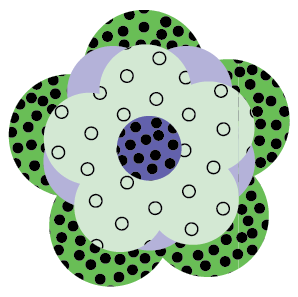
\includegraphics{doooodles_valborg-09.png}
	\end{center}
%\end{wrapfigure}

%-------------------------------
\newpage
\section{Æfingar}
\begin{exercise}\label{set1}
Búið til mengi sem er tómt.
\end{exercise}
\setboolean{firstanswerofthechapter}{true}
\begin{Answer}[ref={set1}]
Þetta eru klækir, þar sem það veldur tvíræðni að nota tóma slaufusviga til að skilgreina bæði tóma orðabók og tómt mengi var ákveðið að tómir slaufusvigar þýddu alltaf orðabók.
En tómamengið er gífurlega mikilvægt, því nauðsynlegt að geta búið það til og átt það svo það er að sjálfsögðu hægt.
Með þessu móti er hægt að búa til tómt mengi.
	\begin{lstlisting}
mengi = set()
	\end{lstlisting}
\end{Answer}
\setboolean{firstanswerofthechapter}{false}


\begin{exercise}\label{set2}
Búið til lista af strengjum og búið svo til mengi út frá þeim lista.
\end{exercise}
\begin{Answer}[ref={set2}]
	Hér þarf einungis að nota lykilorðið til þess að kasta.
	\begin{lstlisting}
listi = ["hér er strengur1", "ólíkur öllum öðrum", "eins", "eins", "Eins", "ekki eins"]
mengi = set(listi)\end{lstlisting}
\end{Answer}


\begin{exercise}\label{set3}
Búið til lista af tölunum 1, 2, 3, 4, 5 og tómt mengi.
Ítrið þá í gegnum talnalistann með for-lykkju þannig að þið rúllið frá 0 upp í töluna 4 (eða einum minna en lengdin á listanum) með \texttt{range} fallinu svo að þið getið skoðað eitt stak hægra megin við þá tölu sem þið eruð að skoða.

Það sem þið gerið í lykkjunni ykkar er að skoða töluna í staki \textit{i} (hlaupandi stakið) og töluna í staki \textit{i+1}.
Leggið þær saman og setjið inn í tóma mengið með \texttt{add} aðferðinni, það á að vera skilgreint fyrir ofan lykkjuna.

Þegar lykkjan er búin að keyra eruð þið komin með talnamengi með nokkrum tölum og svo upphaflega listann.

Kastið listanum í mengi og dragið hann frá (með mínus reiknivirkjanum) frá menginu.

Þið eigið að fá lausnina \{7, 9\}.
\end{exercise}
\begin{Answer}[ref={set3}]
Hér erum við að rifja upp ýmislegt gagnlegt sem gott er að muna.
Það fyrsta er hvernig á að ítra með for-lykkju og hitt er að nota \texttt{range}.
Það sem er hins vegar nýtt er að við notum \texttt{range} til að rúlla upp í 4 því við viljum að 3 sé með en ekki 4.
Ástæðan er sú að hæsti vísirinn í 5 staka lista er 4.
Til þess að geta horft hægra megin við hann má ekki skoða síðasta stakið því það er ekkert stak hægra megin við það.

Að síðustu er þetta spurning um að skoða hvað mengið inniheldur sem listinn gerir ekki.

	\begin{lstlisting}
talnalisti = [1,2,3,4,5]
samlagningarmengi = set()
for i in range(4):

	tala = talnalisti[i] + talnalisti[i+1]
	samlagningarmengi.add(tala)

print(samlagningarmengi - set(talnalisti))\end{lstlisting}
\end{Answer}

\begin{exercise}\label{set4}
Búið til tvö mengi sem innihalda einhverjar tölur og finnið sniðmengi þeirra með því að nota reiknivirkjann \texttt{\&}.
\end{exercise}
\begin{Answer}[ref={set4}]
	Sniðmengið er það sem er sameiginlegt með mengjunum svo mengi með stökin 1,2 á 2 sameiginlegt með mengi sem inniheldur stökin 2,5,6.
\begin{lstlisting}
mengi1 = {1,2,3,4,5,6,7,7,8}
mengi2 = {2,4,7,9,7,6,4,3,4,44,4,44,4,4}
mengi3 = mengi1 & mengi2\end{lstlisting}
\end{Answer}

%\chapterimage{chapter_head_2.pdf} % Chapter heading image

\chapter{Föll}\index{Föll}\label{k:föll}

\section{Tilgangur falla}\index{Tilgangur falla}

\section{Að skrifa föll}

\section{Viðföng}

\section{Skilagildi}

\section{Lokun}



% ---------------------------------------------- 

% SNIÐMÁT

% ----------------------------------------------
%
%\subsection{Descriptions and Definitions}\index{Lists!Descriptions and Definitions}

%\begin{description}
%\item[Name] Description
%\item[Word] Definition
%\item[Comment] Elaboration
%\end{description}

%----------------------------------------------------------------------------------------
%	CHAPTER 2
%----------------------------------------------------------------------------------------

% Búið að gera athugasemd utan um þetta allt
\comment{
\chapter{In-text Elements}

\section{Theorems}\index{Theorems}

This is an example of theorems.

\subsection{Several equations}\index{Theorems!Several Equations}
This is a theorem consisting of several equations.

\begin{theorem}[Name of the theorem]
In $E=\mathbb{R}^n$ all norms are equivalent. It has the properties:
\begin{align}
& \big| ||\mathbf{x}|| - ||\mathbf{y}|| \big|\leq || \mathbf{x}- \mathbf{y}||\\
&  ||\sum_{i=1}^n\mathbf{x}_i||\leq \sum_{i=1}^n||\mathbf{x}_i||\quad\text{where $n$ is a finite integer}
\end{align}
\end{theorem}

\subsection{Single Line}\index{Theorems!Single Line}
This is a theorem consisting of just one line.

\begin{theorem}
A set $\mathcal{D}(G)$ in dense in $L^2(G)$, $|\cdot|_0$. 
\end{theorem}

%------------------------------------------------

\section{Definitions}\index{Definitions}

This is an example of a definition. A definition could be mathematical or it could define a concept.

\begin{definition}[Definition name]
Given a vector space $E$, a norm on $E$ is an application, denoted $||\cdot||$, $E$ in $\mathbb{R}^+=[0,+\infty[$ such that:
\begin{align}
& ||\mathbf{x}||=0\ \Rightarrow\ \mathbf{x}=\mathbf{0}\\
& ||\lambda \mathbf{x}||=|\lambda|\cdot ||\mathbf{x}||\\
& ||\mathbf{x}+\mathbf{y}||\leq ||\mathbf{x}||+||\mathbf{y}||
\end{align}
\end{definition}

%------------------------------------------------

\section{Notations}\index{Notations}

\begin{notation}
Given an open subset $G$ of $\mathbb{R}^n$, the set of functions $\varphi$ are:
\begin{enumerate}
\item Bounded support $G$;
\item Infinitely differentiable;
\end{enumerate}
a vector space is denoted by $\mathcal{D}(G)$. 
\end{notation}

%------------------------------------------------

\section{Remarks}\index{Remarks}

This is an example of a remark.

\begin{remark}
The concepts presented here are now in conventional employment in mathematics. Vector spaces are taken over the field $\mathbb{K}=\mathbb{R}$, however, established properties are easily extended to $\mathbb{K}=\mathbb{C}$.
\end{remark}

%------------------------------------------------

\section{Corollaries}\index{Corollaries}

This is an example of a corollary.

\begin{corollary}[Corollary name]
The concepts presented here are now in conventional employment in mathematics. Vector spaces are taken over the field $\mathbb{K}=\mathbb{R}$, however, established properties are easily extended to $\mathbb{K}=\mathbb{C}$.
\end{corollary}

%------------------------------------------------

\section{Propositions}\index{Propositions}

This is an example of propositions.

\subsection{Several equations}\index{Propositions!Several Equations}

\begin{proposition}[Proposition name]
It has the properties:
\begin{align}
& \big| ||\mathbf{x}|| - ||\mathbf{y}|| \big|\leq || \mathbf{x}- \mathbf{y}||\\
&  ||\sum_{i=1}^n\mathbf{x}_i||\leq \sum_{i=1}^n||\mathbf{x}_i||\quad\text{where $n$ is a finite integer}
\end{align}
\end{proposition}

\subsection{Single Line}\index{Propositions!Single Line}

\begin{proposition} 
Let $f,g\in L^2(G)$; if $\forall \varphi\in\mathcal{D}(G)$, $(f,\varphi)_0=(g,\varphi)_0$ then $f = g$. 
\end{proposition}

}

%------------------------------------------------

%\section{Examples}\index{Examples}

%This is an example of examples.

%\subsection{Equation and Text}\index{Examples!Equation and Text}

%\begin{example}
%Let $G=\{x\in\mathbb{R}^2:|x|<3\}$ and denoted by: $x^0=(1,1)$; consider the function:
%\begin{equation}
%f(x)=\left\{\begin{aligned} & \mathrm{e}^{|x|} & & \text{si $|x-x^0|\leq 1/2$}\\
%& 0 & & \text{si $|x-x^0|> 1/2$}\end{aligned}\right.
%\end{equation}
%The function $f$ has bounded support, we can take $A=\{x\in\mathbb{R}^2:|x-x^0|\leq 1/2+\epsilon\}$ for all %$\epsilon\in\intoo{0}{5/2-\sqrt{2}}$.
%\end{example}

%\subsection{Paragraph of Text}\index{Examples!Paragraph of Text}

%\begin{example}[Example name]
%\lipsum[2]
%\end{example}

%------------------------------------------------


%------------------------------------------------

%\section{Vocabulary}\index{Vocabulary}

%Define a word to improve a students' vocabulary.

%\begin{vocabulary}[Word]
%Definition of word.
%\end{vocabulary}

%----------------------------------------------------------------------------------------
%	PART
%----------------------------------------------------------------------------------------

\part{Seinni hluti - Hlutbundin forritun }

%----------------------------------------------------------------------------------------
%	CHAPTER 3
%----------------------------------------------------------------------------------------

\chapterimage{chapter_head_1.pdf} % Chapter heading image

%\chapterimage{chapters11.png} % Chapter heading image

\chapter{Kóðasöfn}\index{Kóðasöfn}\label{k:import}
\textbf{Kóðasafn} (e. library)\footnote{Hugtökin \textit{package} og \textit{module} ná einnig yfir kóðasöfn í Python vegna þess hve lauslega kóðasöfn eru skilgreind.} er endurnýtanlegur kóði sem útfærir ákveðna virkni og hefur ákveðið samhengi.
Tilgangur þess er að spara forriturum vinnu við að útfæra ýmsa algenga virkni og reiða sig í staðinn á kóða sem er nú þegar til.
Þetta hjálpar okkur við að vera ekki að finna upp hjólið í sífellu.
Ómögulegt er að ætla að forrita að einhverju viti án þess að nota kóðasöfn.

Við notum kóðasöfn með \textbf{import} skipuninni. 
Þegar import hefur verið sett inn einhvers staðar í skjal er óþarfi að setja það inn aftur, venjan er að öll import séu gerð efst í skjali burtséð frá því hvar í skjalinu þau eru notuð.
Það gerir kóðann læsilegri og undirbýr okkur við fyrir því sem er að fara að gerast.
Ef það stendur til dæmis efst í skjali að kóðasöfnin \textit{math} og \textit{random} séu notuð vitum við strax að í þessum kóða er líklega verið að vinna með handahófskennd og stærðfræði, en ef efst stæði að kóðasöfnin \textit{datetime} og \textit{time} væru notuð erum við líklega að skoða kóða sem er að vinna með tíma og dagsetningar, það ætti þá ekki að koma okkur á óvart að sjá dagsetningarvinnslu.

Venjan að setja öll import efst er því gagnleg fyrir þær sakir að kóðinn verður læsilegur og auðveldara verður að halda utan um kóðasöfnin sem við erum að nota.

\section{Notkun kóðasafna}\index{Tilgangur kóðasafna}\label{uk:kóðasöfn-kynnt}
Eins og kom fram í kynningu þá viljum við geta einbeitt okkur að því að leysa okkar vandamál í stað þess að finna upp hjólið og því viljum við kynna okkur þau kóðasöfn sem eru í boði sem útfæra virkni sem við viljum beita.

Tilgangur þeirra er að létta okkur lífið og gera virkni aðgengilega.
Í næsta undirkafla verða tekin fyrir nokkur gagnleg kóðasöfn en við getum varla talað um tilgang og gagnsemi kóðasafna án þess að taka eitthvert þeirra fyrir.
Í inngangi voru kóðasöfnin \texttt{time} og \texttt{random} nefnd.
Skoðum þau aðeins núna, sjá kóðabúta \ref{lst:kóðasöfn-kynnt-time} og \ref{lst:kóðasöfn-kynnt-rand} þar sem kóðasöfnin eru tekin fyrir.
Þau bjóða bæði upp á aragrúa aðferða og eiginda sem er út fyrir efni þessarar bókar en þó þess virði að taka fyrir ákveðna virkni sem búist er við að nota í æfingum í lok kaflans.
\paragraph{}
Um kóðasafnið time:

\begin{itemize}
	\item \texttt{time.time()} skilar okkur því hversu margar sekúndur eru síðan tímatal í tölvum hófst 1. jan 1970.
	\item \texttt{time.sleep()} tekur við tölu og lætur vélina bíða í svo margar sekúndur áður en hún framkvæmir aðgerðina í næstu línu fyrir neðan.
	\item \texttt{time.localtime()} skilar okkur nd sem inniheldur í minnkandi röð hver tíminn er, frá ári niður í sekúndur, ásamt deginum í vikunni og árinu, síðasta er gildi sem tekur mið af \texttt{isdaylightsavingstime} (\textbf{isdst}).
\end{itemize}

\paragraph{}
Um kóðasafnið random: Þetta kóðasafn gerir forriturum auðveldara fyrir með því að gera \textit{handahófskennd} (e. randomness) aðgengilega, en það að geta gert hluti af handahófi er mjög mikilvægt í tölvunarfræði og forritun.

\begin{itemize}
	\item \texttt{random.randint()} nær í heiltölu á lokuðu bili, þar sem báðir endapunktar eru teknir með.
	\item \texttt{random.random()} nær í fleytitölu á bilinu 0-1.
	\item \texttt{random.choice()} nær í stak af handahófi upp úr ítranlegum hlut.
	\item \texttt{random.shuffle()} stokkar upp í raðanlegum hlut.
\end{itemize}
\vspace{1cm}
\begin{lstlisting}[caption=Notkun kóðasafna með time, label=lst:kóðasöfn-kynnt-time]
import time

sekundur_adan = time.time()
time.sleep(3)
sekundur_3_sek_eftir_adan = time.time()

thrir = sekundur_3_sek_eftir_adan - sekundur_adan
print(thrir)
\end{lstlisting}
\lstset{style=uttak}
\begin{lstlisting}
3.001107931137085
\end{lstlisting}
\lstset{style=venjulegt}
\vspace{1cm}
Þið fáið ekki nákvæmlega sömu tölu, ekki einu sinni ef þið reynið að keyra þetta oft. Það er líka ómögulegt að ná keyrslu upp á millisekúndunákvæmni með þessu móti.

Skoðum næst handahófskennd.

\phantom{easter egg}
%\begin{wrapfigure}{i}{0.2\textwidth} %i o r l 
\begin{center}
	
\includegraphics[scale=1.9]{doodles31-28.png}
\end{center}
%\end{wrapfigure}
\phantom{}

\begin{lstlisting}[caption=Notkun kóðasafna með random, label=lst:kóðasöfn-kynnt-rand]
import random

listi = [1,2,3,4,5,6,7,8,9]
einhver_tala = random.choice(listi)
random.shuffle(listi)
print(listi)
for i in range(einhver_tala):
	if random.randint(min(listi),max(listi)) > i:
		print("Þú vannst 10kr")
	else:
		print("Þú þarft að ydda blýantana þína")

fjoldi_folks = 100
hlutfall_folks_med_raudan_trefil = fjoldi_folks*random.random()
print(hlutfall_folks_med_raudan_trefil)
\end{lstlisting}
\lstset{style=uttak}
\begin{lstlisting}
[9, 3, 2, 7, 5, 1, 4, 8, 6]
Þú vannst 10kr
Þú vannst 10kr
Þú vannst 10kr
Þú vannst 10kr
Þú þarft að ydda blýantana þína
Þú þarft að ydda blýantana þína
Þú þarft að ydda blýantana þína
Þú þarft að ydda blýantana þína
98.19660121258345 %
\end{lstlisting}
\lstset{style=venjulegt}

Sama er upp á teningnum hér, úttakið verður ekki það sama þegar þið keyrið þennan kóða en ekki af sömu ástæðu.
Hér er það beinlínis ætlunarverkið að úttakið verði óútreiknanlegt.



Eins og sést í kóðabút \ref{lst:kóðasöfn-kynnt-time} þarf að nota nafnið á kóðasafninu til að ná í aðferðir og virkni.
Sum kóðasöfn heita löngum nöfnum og ef fólk vill stytta nöfnin á þeim má nota lykilorðið \textbf{as} til þess að varpa nafninu á kóðasafninu í annað breytuheiti, sjá notkun í kóðabút \ref{lst:kóðasöfn-as}.
Vísunin kemur strax þegar kóðasafnið er flutt inn og þar eftir er kóðasafnið aðgengilegt með þessari vísun.
Þá er mikilvægt að hafa í huga að nefna kóðasöfnin eittvað sem verður ekki óvart yfirskrifað í kóðanum og gæti valdið ruglingi, eins og að skipta út \texttt{import random} fyrir \texttt{import random as listinn\_minn}.
Það væri hrikalegt, illlæsilegt og myndi fyrirsjáanlega valda vandamálum.
Nú vitum við hvernig á að nota kóðasöfn.

\begin{lstlisting}[caption=Lykilorðið as, label=lst:kóðasöfn-as]
import random as rnd
import time as t

timi = t.time() 
tala = rnd.random()
print(timi * tala % tala)
\end{lstlisting}
\lstset{style=uttak}
\begin{lstlisting}
0.4772097503672992
\end{lstlisting}
\lstset{style=venjulegt}

\section{Nokkur gagnleg kóðasöfn}\index{Nokkur gagnleg kóðasöfn}\label{uk:kóðasöfn-gagnleg}
Tilgangur þessarar bókar er ekki að tiltaka hvert einasta kóðasafn sem er til, heldur að kynna til sögunnar hvernig notkun þeirra virkar og einhver þau algengustu eða skemmtilegustu kóðasöfn sem eru notuð í dag.
Þetta er gert til þess að halda bókinni frá því að verða eins og símaskrá (ef einhver lesandi man eftir að hafa haldið á símaskrá) og passa að hún haldi í við þróun í fræðigreininni.

Að því sögðu er hér stutt kynning á nokkrum vinsælum kóðasöfnum.

\begin{itemize}
	\item \textbf{math}, gerir aðgengilegar alls konar stærðfræðilegar aðgerðir, eins og hornaföll, logra, veldisföll og tölulega vinnslu.
	Ásamt því gefur það okkur aðgengi að mikilli nákvæmni á hinum ýmsu rauntölustærðum eins og pí.
	\item \textbf{numpy}, gerir stærðfræðilega vinnslu aðgengilega, t.d. á fylkjum.
	Numpy er sérhæft fyrir flóknari vinnslu en math.
	\item \textbf{scipy}, er það sem hægt er að nota til þess að vinna með \textit{vélanám} (e. machine learning).
	Scipy hefur oft verið sagt óþarflega flókið í notkun, en hugmyndirnar sem þar er verið að vinna með eru í grunninn mun flóknari en í numpy og math pökkunum svo það ætti ekki að koma á óvart.
	\item \textbf{pygame}, er kóðasafn sem vinnur með grafískt viðmót og inntak frá notanda oft með mjög skapandi útkomu.
	Margir litlir leikir hafa orðið til með þessu kóðasafni og er til mýgrútur af dæmum og leikjum á netinu til að vinna út frá.
	\item \textbf{datetime}, vinnur með dagsetingar því ef við ætlum einhvern tímann að skrifa hugbúnað sem vinnur með dagsetningar viljum við alls ekki finna upp hjólið.
	Þar er tekið á sumar- og vetrartíma, hlaupárum og öðru slíku sem við viljum ekki þurfa að hafa áhyggjur af.
	\item \textbf{matplotlib}, er safn sem var búið til í kringum tvívíða sýn á gögn  til að sýna gröf og til að gera gögn sýnileg á fjölbreytilegan máta.
	Þetta er annað safn sem hefur slæmt orð á sér fyrir að vera óþarflega óaðgengilegt.
\end{itemize}

Það er út fyrir efni bókarinnar að sýna hvernig eigi að búa til kóðasöfn sem eru nothæf öðrum, en það er lítið mál að kynna sér það á vefnum.

%-------------------------------
\newpage
\section{Æfingar}

\begin{exercise}\label{imp1}
Notið input skipun til þess að komast að því hvort að notandinn viti hversu lengi 10 sekúndur eru að líða. 
\end{exercise}
\setboolean{firstanswerofthechapter}{true}
\begin{Answer}[ref={imp1}]
input skipunin er í rauninni bara þarna í staðinn fyrir time.sleep(), núna er það notandinn sem ákveður hvenær næsta lína af kóða er keyrð.
Það sem við þurfum að fatta er að reikna rétt út og finna tímann.
	\begin{lstlisting}
adan = time.time()
input("ýttu eftir 10 sek")
nuna = time.time()
print(nuna-adan)\end{lstlisting}
\end{Answer}
\setboolean{firstanswerofthechapter}{false}


\begin{exercise}\label{imp2}
Gefinn er eftirfarandi listi: 
['Lorem','ipsum','dolor','sit','amet,','consectetur',
'adipiscing','elit,','sed','do','eiusmod','tempor',
'incididunt','ut','labore','et','dolore','magna','aliqua.',
'Ut','enim','ad','mini','veniam,','quis','nostrud',
'exercitation','ullamco','laboris','nisi','ut','aliquip',
'ex','e','commodo','consequat.','Duis','aute','irure',
'dolor','in','reprehenderit','in','voluptate','velit',
'esse','cillum','dolore','eu','fugiat','nulla','pariatur.',
'Excepteur','sint','occaect','cupidatat','non','proident,',
'sunt','in','culpa','qui','officia','deserunt','mollit',
'ani','id','est','laborum.']

Náið í orð af handahófi úr listanum og náið svo í tákn af handahófi úr því orði.
\end{exercise}
\begin{Answer}[ref={imp2}]
Hér þurfum við aðallega að átta okkur á því hvaða föll við viljum nota úr random pakkanum, úr listanum viljum við nota choice en til að finna eitthvað tákn viljum nota randint.
Athugum hér að þegar við notum randint þá gefum við upp bil af tölum eins og 1,10 þá eru bæði 1 og 10 með, svo þegar við notum það til að búa til sætisvísi af handahófi verðum við að passa að fara ekki út fyrir löglega sætisvísa.
	\begin{lstlisting}
rugl_ord = random.choice(listi)
rugl_takn = rugl_ord[random.randint(0,len(rugl_ord)-1)]
print(rugl_ord, rugl_takn)\end{lstlisting}
\end{Answer}

%\chapterimage{chapter_head_2.pdf} % Chapter heading image

\chapter{Skjalavinnsla}\index{Skjalavinnsla}\label{k:skjalavinnsla}
Að vinna með skjöl án þess að hafa þau opin í ritli, eins og MS Word, LibreOffice Write, Notepad eða álíka, er mjög ákjósanlegt ef t.d. þarf að gera litla breytingu í stóru skjali eða einhverja breytingu í mjög mörgum skjölum (skilgreiningin á mjög mörgum er sveiginaleg, sumum finnst það vera að gera eitthvað oftar en þrisvar).
Segjum sem svo að við hefðum skrifað ritgerð og við yfirlestur á henni tækjum við eftir að við gerðum eina ákveðna villu alltaf.
Villan væri að við hefðum gleymt að setja stóran staf í upphafi allra setinganna okkar!
Ó nei, hvernig tókst okkur að gleyma þessu?
Það á eftir að taka óratíma að lesa yfir og laga hvern einasta staf því ritgerðin er 20 blaðsíður.
En vegna þess að við erum snjöll og kunnum að vinna með strengi þá getum við gert þetta með hjálp Python.

Hægt er að búa til skjöl, opna þau, lesa þau, skrifa inn í þau, yfirskrifa þau, loka þeim og henda þeim.
Þetta er mikilvægt vegna þess að við viljum geta sagt tölvunni að nálgast skjöl og gera eitthvað við þau, við viljum ekki þurfa að handstýra tölvunni að óþörfu, til dæmis með því að lesa sjálf yfir 20 blaðsíður í leit að litlum staf þar sem á að vera stór.
Til þess er tölvan.

\begin{lstlisting}[caption=Hér sjáum við hvernig má búa til skjöl, label=lst:skjalavinnsla-kynning]
skjal = open('skjal1.txt', mode = 'w+') 

skjal.write('hér kemur eitthvað sem við viljum setja inn í skjalið okkar')

skjal.close()
\end{lstlisting}

Nú getum við séð, á sama stað og þessi kóði er keyrður, í skrársafninu (e. filesystem) okkar skjal sem heitir \texttt{skjal1.txt} vegna þess að við völdum það nafn í línu 1 innan svigans, ástæðan fyrir því að þarna stendur \emph{.txt} er sú að sú skráarending er fyrir einföld textaskjöl\footnote{svipað eins og .doc sem við könnumst flest við}.
Þar kemur einnig fram \texttt{mode} sem er valið sem \texttt{w+}, sem leyfir okkur að lesa og skrifa eða yfirskrifa.
Við veljum máta sem hentar okkur hverju sinni, þeir sem eru í boði eru:
\begin{itemize}
	\item \textbf{r} : leyfir okkur aðeins að lesa (read).
	\item \textbf{w} : leyfir okkur aðeins að skrifa (write).
	\item \textbf{a} : leyfir okkur aðeins að bæta við aftast (append).
	\item \textbf{r+} : leyfir okkur að lesa og skrifa (read +).
	\item \textbf{w+} : leyfir okkur að lesa og skrifa og yfirskrifar (write +).
\end{itemize}

Við tökum einnig eftir í kóðabút \ref{lst:skjalavinnsla-kynning} að við notum þrjú föll, fallið \texttt{open()} er það sem býr til skjalið með w+ og nafninu sem við gefum því, þá er skjalið opið og aðgengilegt.
Þá köllum við í \texttt{write} sem skrifar inn í skjalið, sú skipun er í boði vegna þess að við notuðum w+ (er ekki möguleg fyrir r t.d.).
Við erum vissulega bara að gera einfalda hluti en þetta er til að sýna virknina í grunninnn ekki til að finna upp hjólið.
Svo að lokum sjáum við eitthvað áhugavert, það er \texttt{close()}.
Til hvers að gera það?
Hafið þið lent í því að við það að reyna að henda skjali í ruslið af tölvunni ykkar fáið þið villu um að það sé ekki hægt því að skjalið er opið einhversstaðar?
Það er það sem við erum að fyrirbyggja hérna með því að loka skjalinu þegar við erum búin að vinna með það.
Við erum í rauninni bara að ganga frá eftir okkur svo að það sé ekki eitthvað opið sem er fyrir.

\section{Unnið með skjöl}\index{Unnið með skjöl}\label{uk:skjalavinnsla-kynnt}
Til þess að geta unnið með skjöl þurfum við að geta vísað í þau, til þess notum við breytur.
Eins og breytan \texttt{skjal} í kóðabúr \ref{lst:skjalavinnsla-kynning}.
Breytan okkar stendur þá ekki fyrir einhverja grunntýpu í Python heldur er það vísun í heilt skjal á skráarsafninu okkar.

Í kóðabút \ref{lst:skjalavinnsla-open} koma fram nokkrar aðferðir sem Python býður upp á fyrir skjöl sem búið er að opna.
Til þess að sækja upplýsingar úr skrá þarf tölvan að lesa hana.
Við tökum eftir því að þar er eitthvað til sem heitir \textit{seek}, ástæðan fyrir því að við þurfum það er að tölvan les frá vinstri til hægri eins og henni er sagt en ef hún á að lesa eitthvað aftur frá byrjun eða öðrum stað þá þarf að segja henni að færa leshausinn sinn þangað.
Nú er hætta á því að enginn lesandi hafi nokkurn tímann séð segulband en hugmyndin þar er sú sama, tölvan sem les segulbandið getur bara lesið bandið sem er undir leshausnum og sér ekkert annað.
Ef tölvan á að lesa einhvern annan hluta af segulbandinu þarf að spóla fram eða til baka.
Sama er upp á teningnum hérna, við þurfum að stilla leshausinn fyrir framan það gildi sem við viljum lesa hverju sinni.
Ef vélin er búin að lesa skjalið er leshausinn kominn út í enda og við getum ekki lesið meira nema færa hann.

Þetta er svipað því eins og ef við settum puttann niður í bók og mættum bara lesa orðin fyrir ofan puttann og svo bara til hægri, þá til að lesa eitthvað aftur eða fara lengra inn í bókina þyrftum við að taka upp puttann og færa hann þangað.

Byrjum á að gera textaskjalið okkar aðeins bitastæðara með því að keyra eftirfarandi kóða í sér sellu í vinnubók\footnote{virkar aðeins í Jupyter Notebooks og er ekki sér Python fyrirbæri heldur sérstætt fyrir þessar vinnubækur, þetta leyfir okkur að sleppa við $\backslash$n eða newline character og æfingar tengdum því}:
\begin{verbatim}
%%writefile skjal1.txt
hér kemur eitthvað sem við viljum setja inn í skjalið okkar
hér er næsta lína í skjalinu
úps engin lína endar á punkti og engin lína hefst á stórum staf
En nú lagast það.
æ, það gleymdist stór stafur.
Og nú gleymdist punktur
\end{verbatim}

Skoðum svo hvað hægt er að gera við þennan texta\footnote{Þarna kemur fram annað viðfang sem heitir encoding, þarna er það valið sem utf-8 sem er það táknasafn sem nær yfir alla séríslenka stafi. Ef þið lendið í vandræðum við að íslenskir stafir eru í ruglinu er gott að vita til þess að stafakóðunin er þá mögulega önnur en utf-8. Þetta á alls ekki bara við um Python heldur er þetta alþjóðlegur staðall sem nýtist hvarvetna.}.

\begin{lstlisting}[caption=Hér sjáum við einfalda skjalavinnslu, label=lst:skjalavinnsla-open]
vinnuskjal = open('skjal1.txt', encoding = 'utf-8', mode = 'r')	

linurnar = vinnuskjal.readlines()
vinnuskjal.seek(150)
print(vinnuskjal.read())

for lina in linur:
	if lina[0].islower() and lina[-1] != ".":
		print("línan byrjar á litlum staf og endar ekki á punkti")
	elif lina[0].islower() or lina[-1] != ".":
		print("línan endar ekki á punkti eða byrjar á litlum staf")
	else:
		print(lina)

vinnuskjal.close()
\end{lstlisting}
\lstset{style=uttak}
\begin{lstlisting}
t á stórum staf
En nú lagast það.
æ, það gleymdist stór stafur.
Og nú gleymdist punktur

línan byrjar á litlum staf og endar ekki á punkti
línan byrjar á litlum staf og endar ekki á punkti
línan byrjar á litlum staf og endar ekki á punkti
línan endar ekki á punkti eða byrjar á litlum staf
línan byrjar á litlum staf og endar ekki á punkti
línan endar ekki á punkti eða byrjar á litlum staf
\end{lstlisting}
\lstset{style=venjulegt}

Í kóðabút \ref{lst:skjalavinnsla-open} eru teknar fyrir þær helstu aðferðir sem eru í boði fyrir lestur á skjali \texttt{read()} og \texttt{readlines()}, annað gefur okkur streng en hitt gefur okkur lista af línum sem við getum ítrað í gegnum.
Takið eftir því að leshausinn er settur á stað 150 og svo er útkoman prentuð, en það hefur ekki áhrif á \texttt{linur} því að sú breyta var skilgreind þegar leshausinn var á 0 og færðist út í enda við það að nota \texttt{readlines()}.
Prófið ykkur áfram með röðunina á kóðalínunum.
 
Það gæti verið vesen að þurfa að muna eftir því að loka skjalinu og því viljum við skoða annan möguleika með nýju lykilorði \textbf{with}, við höfum séð \textbf{as} sem býr til \textit{alias} eða annað heiti.
Sjáum kóðabút \ref{lst:skjalavinnsla-open-as}, þar sem öll vinnslan í skjalinu tilheyrir inndrætti undir \texttt{with} og \texttt{as}.
Þetta er eins og með föll, þegar við skrifum eitthvað í sama inndrætti og í línu 1 þá erum við komin út fyrir skjalavinnsluna okkar og skjalið er ekki lengur aðgengilegt því þá er verið að reyna að vinna með skrá sem er lokuð.
 
\begin{lstlisting}[caption=Hér sjáum við nýja leið til að opna skjal og loka því sjálfkrafa, label=lst:skjalavinnsla-open-as]
with open('skjal1.txt', encoding='utf-8') as test:
	efni = test.read()
	test.seek(0)
	efni_i_listum = test.readlines()

with open('skjal1.txt', encoding='utf-8', mode= 'w+') as blergh:
	efni = blergh.write('Ég yfirskrifaði allt og á nú skjal sem heitir það sama en inniheldur bara þetta')
	blergh.seek(0)
	efni_i_listum2 = blergh.readlines()

print(efni_i_listum)
print(efni_i_listum2)
\end{lstlisting}
\lstset{style=uttak}
\begin{lstlisting}
['hér kemur eitthvað sem við viljum setja inn í skjalið okkar\n', 'hér er næsta lína í skjalinu\n', 'úps engin lína endar á punkti og engin lína hefst á stórum staf\n', 'En nú lagast það.\n', 'æ, það gleymdist stór stafur.\n', 'Og nú gleymdist punktur\n']
['Ég yfirskrifaði allt og á nú skjal sem heitir það sama en inniheldur bara þetta']
\end{lstlisting}
\lstset{style=venjulegt}

Tökum eftir hér að við fáum villu við að reyna að vísa í breyturnar \texttt{test} og \texttt{blergh} en hinar breyturnar sem við búum til á meðan vinnslunni stendur eru enn aðgengilegar eins og sést í línum 12 og 13.

En þá skulum við skoða hvernig við eigum að fara að því að laga textann án þess að opna skjalið handvirkt og breyta táknunum sjálf.
Það sem við vitum er að fremsti stafur á alltaf að vera stór og aftasta táknið á alltaf að vera punktur.
Við getum svo breytt handvirkt þeim fáeinu setningum sem við viljum að endi á spurningarmerki eða upphrópunarmerki.

\begin{lstlisting}[caption=Leysum punkta og hástafa vandann okkar, label=lst:skjalavinnsla-lausn]
with open('skjal1.txt', encoding='utf-8', mode= 'r') as lausn:
	lausn.seek(0)
	linur = lausn.readlines()
	for lina in linur:
		i = linur.index(lina)
		lina = lina[0].upper() + lina[1:]
		if lina[-2] != ".":
			lina = lina[:-1] + "." + lina[-1]
		linur[i] = lina

with open('skjal1.txt', encoding = 'utf-8', mode = 'w+') as laga:
	laga.writelines(linur)
	laga.seek(0)
	print(laga.read())
\end{lstlisting}
\lstset{style=uttak}
\begin{lstlisting}
Hér kemur eitthvað sem við viljum setja inn í skjalið okkar.
Hér er næsta lína í skjalinu.
Úps engin lína endar á punkti og engin lína hefst á stórum staf.
En nú lagast það.
Æ, það gleymdist stór stafur.
Og nú gleymdist punktur.
\end{lstlisting}
\lstset{style=venjulegt}

Athugið sérstaklega notkun á -1 og -2, athugið hvað gerist ef þið breytið því, þetta er útaf því að síðasta táknið er ,,new line character'' eða $\backslash$n (þó þetta eru í raun tvö tákn þá er þetta saman eitt tákn).
Þó það hefði mögulega verið minni hausverkur að laga þessar fáeinu setningar og að læra rétta stafsetningu þá er pælingin hérna var að við vorum búin að gera þetta síðustu tuttugu blaðsíðurnar og við vildum alls ekki gera einhverja villu í yfirferðinni með því að gleyma punkti einu sinni því að það fór framhjá okkur.
Við ættum að temja okkur að láta tölvuna sjá um allt það sem við erum fær um að útskýra fyrir henni hvernig eigi að gera.

%-------------------------------
\newpage
\section{Æfingar}

\begin{exercise}\label{doc1}
Búiið til skjal með .txt endingu, setjið inn í það nokkrar mismunandi línur (annað hvort með \%\%writefile eða annarri leið og munið þá eftir $\backslash$n til þess að fá mismunandi línur).
Lykkjið svo í gegnum línurnar og prentið út þær sem byrja á sérhljóða.
\end{exercise}
\setboolean{firstanswerofthechapter}{true}
\begin{Answer}[ref={doc1}]

	\begin{lstlisting}
%%writefile doc1.txt
Þessi byrjar ekki á sérhljóða
En þessi gerir það
\end{lstlisting}
\begin{lstlisting}´
with open('doc1.txt', mode = 'r') as doc1:
linur = doc1.readlines()
for lina in linur:
if(lina[0].lower() in 'aáeéiíoóuúyýæö'):
print(lina)\end{lstlisting}
\end{Answer}
\setboolean{firstanswerofthechapter}{false}


\begin{exercise}\label{doc2}
Búið til textaskjal sem inniheldur söngtexta úr einhverju lagi (þá er gott að nota \%\%writefile), lesið svo skjalið og geymið línurnar í lista.
Prentið svo eina línu af handahófi úr listanum.
\end{exercise}
\begin{Answer}[ref={doc2}]
	\begin{lstlisting}
%%writefile doc2.txt
Krummi svaf í klettagjá,
kaldri vetrarnóttu á,
::verður margt að meini::
Fyrr en dagur fagur rann,
freðið nefið dregur hann
::undan stórum steini.::

Allt er frosið úti gor,
ekkert fæst við ströndu mor
::svengd er metti mína.::
Ef að húsum heim ég fer
heimafrakkur bannar mér
::seppi' úr sorp að tína.::

Öll er þakin ísi jörð,
ekki séð á holtabörð
::fleygir fuglar geta.::
En þó leiti út um mó,
auða hvergi lítur tó;
::hvað á hrafn að éta.::

Á sér krummi ýfði stél,
einnig brýndi gogginn vel,
::flaug úr fjallagjótum::
Lítur yfir byggð og bú
á bænum fyrr en vakna hjú,
::veifar vængjum skjótum.::

Sálaður á síðu lá
sauður feitur garði hjá,
::fyrrum frár á velli.::
Krunk, krunk, nafnar, komið hér,
krunk, krunk, því oss búin er
::krás á köldu svelli.::		
\end{lstlisting}
	\begin{lstlisting}
import random 
with open('doc2.txt', mode = 'r') as doc2:
	linur = doc2.readlines()
	print(random.choice(linur))
\end{lstlisting}
\end{Answer}

%\chapterimage{chapter_head_2.pdf} % Chapter heading image

\chapter{Klasar og hlutir}\index{Klasar og hlutir}\label{k:klasar}
Forritun snýst um að meðhöndla gögn, hingað til höfum við kynnst nokkrum gagnatögum (t.d. strengir og listar), þær gegna mismunandi hlutverkum og bjóða upp á mismunandi aðgerðir til að vinna með gögnin.
Þessar innbyggðu týpur duga þó ekki alltaf og því er mikilvægt að vita að þegar við forritum getum við smíðað okkar eigin.
Þannig getum við aðlagað týpurnar okkar að þeim gögnum sem forritið okkar meðhöndlar og útfært okkar eigin aðferðir á þær.
Klasar gera forriturum kleift að skilgreina sína eigin hluti í flestum hlutbundnum málum, Python er hlutbundið forritunarmál.
Til þess að læra á hvernig eigi að búa til klasa þarf að átta sig á til hvers þeir eru nytsamlegir.

Gagnlegt er að hugsa sér klasa sem skilgreiningu eða uppskrift alveg eins og föll.
Skilgreiningin ein og sér gerir ekki neitt, það er ekki fyrr en við búum okkur til ákveðna útgáfu sem við getum farið að vinna með hana.
Gott dæmi um það er skilgreiningin á rétti á matseðli á veitingastað, textinn á matseðlinum er eingöngu hvað er í boði en er ekki útgáfa af matnum sjálfum.

Klasar eru hlutir sem hugsaðir eru til þess að búa til eintök af og geyma þannig eitthvert ástand og mögulega hafa áhrif á það.
Hugmyndin er að eiga hlut eða \emph{tilvik}, eina tiltekna útgáfu, sem má framkvæma aðgerðir á og eitthvað ástand hlutarins breytist eftir því hvað var gert, þannig er hægt að búa til mörg eintök af sama klasanum og láta hvert tilvik verða fyrir mismunandi áhrifum\footnote{Athuga þarf sérstaklega gildissvið þegar klasar eru annarsvegar, gildissvið í Python geta verið ögn ruglingsleg en við munum ekki beita klösum á það sérhæfðan máta að við lendum í miklum vandræðum.
Hér er tilvalið að skoða ,,meta programming''}.

\section{Klasar skilgreindir}\index{Klasar skilgreindir}\label{uk:klasar-skilgreindir}

Klasar nota lykilorðið \textbf{class} og eru skilgreindir með því orði, allt sem tilheyrir klasanum er inndregið undir honum.
Nöfn klasa eru með stórum staf í Python og flestum hlutbundnum forritunarmálum.

\begin{lstlisting}[caption=Klasinn Bíll skilgreindur, label=lst:klasar-skilgreindir-tegund]
class Bíll:
	tegund = "Citroen"

fyrsti_billinn = Bíll()
print(fyrsti_billinn.tegund)
\end{lstlisting}
\lstset{style=uttak}
\begin{lstlisting}
Citroen
\end{lstlisting}
\lstset{style=venjulegt}

Hugsum okkur að við búum til skilgreiningu á bíl, hann þarf að vera af einhverri tegund, skoðum línur 1-2 í kóðabút \ref{lst:klasar-skilgreindir-tegund}.
Svo viljum við fá tilvik af skilgreiningunni í hendurnar (lína 4), þá búum við til breytu sem fær gildi eins og við höfum gert hundrað sinnum áður, nema núna er gildið sem breytan fær nafnið á klasanum okkar ásamt svigum eins og við séum að kalla í hann.
Prófið núna að búa til annað tilvik af klasanum \texttt{Bíll} án þess að nota svigana og prófið þá að prenta út það sem \texttt{type} skilar fyrir breyturnar tvær.

\begin{lstlisting}[caption=Klasinn Bíll skilgreindur og tvö tilvik búin til, label=lst:klasar-skilgreindir-subaru]
class Bíll:
	tegund = "Citroen"
	
fyrsti_billinn = Bíll()
print(fyrsti_billinn.tegund)
annar_bill = Bíll()
annar_bill.tegund = "Subaru"
print(annar_bill.tegund)
\end{lstlisting}
\lstset{style=uttak}
\begin{lstlisting}
Citroen
Subaru
\end{lstlisting}
\lstset{style=venjulegt}

Breytan \texttt{fyrsti\_bilinn} kemur ekki í veg fyrir það að við getum átt fleiri bíla, en hún heldur utan um ástandið á nákvæmlega þessum bíl okkar.
Segjum að við fáum okkur svo annan bíl, þá getum við búið til aðra breytu (lína 6) í kóðabút \ref{lst:klasar-skilgreindir-subaru} fyrir annað tilvik af klasanum.
Bílarnir eru, fyrir okkur, óaðgreinanlegir í línu 6\footnote{Þar sem ekki hefur verið útfærð \_\_eq\_\_ aðferðin þá er notast við id() fallið úr type klasanum sem klasinn okkar erfir frá bakvið tjöldin.
Við skoðum erfðir betur seinna í kaflanum.} en það breytist svo snarlega þegar við endurskilgreinum \emph{klasabreytuna}\footnote{Í öðrum hlutbundnum málum er venjulega talað um klasafasta en í Python er auðvelt að breyta þeim svo við hæfi að nota annað orð en klasa\textbf{fasti}} í línu 7, \texttt{tegund}.

Prófið nú að skipta um gildi á klasabreytunni \texttt{tegund} fyrir ykkar eigið tilvik af \texttt{Bíll}.

Þá skulum við skoða dálítið sérkennilegt fyrirbæri í Python, það er að við getum endurskilgreint klasabreyturnar okkar, sem hefur áhrif á öll tilvikin okkar.
Til að skoða það skulum við nota aftur kóðann úr kóðabút \ref{lst:klasar-skilgreindir-tegund}.

\begin{lstlisting}[caption=Endurskilgreining á því sem klasinn býður upp á, label=lst:klasar-skilgreindir-tegund2]
class Bíll:
	tegund = "Citroen"
	
fyrsti_billinn = Bíll()
print(fyrsti_billinn.tegund)
Bíll.tegund = "Volvo"
print(fyrsti_billinn.tegund)
\end{lstlisting}
\lstset{style=uttak}
\begin{lstlisting}
Citroen
Volvo
\end{lstlisting}
\lstset{style=venjulegt}

Hér sjáum við hvernig tilvikið okkar, \texttt{fyrsti\_billinn}, af bílaklasanum breytist.
Í línu 5 er \texttt{tegund} "Citroen" en í línu 7 er það orðið að "Volvo".
Þetta gerist því að tilvikið okkar er af þessum klasa og klasinn breyttist í línu 6.
Við endurskilgreindum klasann og því breytast öll tilvik af honum í samræmi.

Nú eigum við tvær breytur sem við getum unnið með, kannski setja bensín á bílinn eða fylla á rúðuvökva og þá gerum við það við þá tilteknu breytu sem við ætlum að framkvæma þá aðgerð á.
En þessi skilgreining innihélt engar aðferðir, við sjáum það í hluta  \ref{uk:klasar-aðferðir}.

\comment{
	
	--------------

Við munum svo beita klösum á hnitmiðaðri máta með svo kölluðum \textit{töfra aðferð} (e. magic method, double underscore method, dunder method\footnote{þarna er orðunum double og under skeytt saman í dunder}) og skoða hvernig á að útbúa hlut með ákveðnum grunnupplýsingum.

Áður en við höldum svo langt skulum við byrja á að skoða orðið \texttt{self} sem er ekki frátekið lykilorð heldur er það hefð og venja að nota það orð til að segja klasanum að nú sé hann að nota sig sjálfan (sjá endurkvæmni í kafla \ref{k:reiknirit})\footnote{Skipta má út orðinu self fyrir hvað sem er, en það þarf þá að halda samhengi, best er að venja sig á nota self svo kóðinn verði læsilegri}.

-----------

}

\comment{
	
------------------------
	
Við sáum þetta í \ref{lst:klasar-self} þegar búið að er að setja fall inn í klasann, við munum hvernig föll eru skilgreind úr kafla \ref{k:föll}, hvernig þau vinna með viðföng og hvernig á að kalla í þau.

\begin{lstlisting}[caption=Klasar , label=lst:klasar-self]
class Tala():
	x = 5
	def leggja_saman(self, x):
		print(self.x + x)

talan_min = Tala()
talan_min.leggja_saman(6)
\end{lstlisting}
\lstset{style=uttak}
\begin{lstlisting}
11
\end{lstlisting}
\lstset{style=venjulegt}

Við sjáum að fallið tekur við tveimur viðföngum \texttt{self} og \texttt{x}.


Tökum eftir hvernig breytan \texttt{t} er skilgreind í kóðabút \ref{lst:klasar-skilgreindir2}, hún er skilgreind eins og hvaða önnur breyta sem við höfum búið til áður.
En það sem kemur hinu megin við jafnaðarmerkið er eins og verið sé að kalla í fall.
Eina sem gefur til kynna að þetta sé ekki fall er að Klasi er með stórum staf.
Ef við gleymum að gera svigana þá fáum við ekki eintak af klasanum til að vinna með heldur fáum við nýja vísun á klasann sjálfan.
Það er við erum með nýtt nafn sem gerir það sama og breytan \texttt{Tala} gerir, annan vísi á \texttt{Tala} en ekki útgáfu til að vinna með.

Það er nafnavenja í Python að klasar séu nefndir með stórum staf, það auðveldar lestur fyrir mannfólk.

Þá sjáum við að í línu 7 er kallað í aðferðina \texttt{leggja\_saman}, hún tekur við einu viðfangi.
En ef við skoðum skilgreininguna á aðferðinni þá eru þar skilgreind tvö viðföng.
Fyrra viðfangið \texttt{self} er þarna notað fyrir klasann til að vita að það sé verið að tala um hann sjálfan, svo þarna inni eru tvö mismunandi x.
Fyrra x-ið er úr línu 2 og seinna x-ið er úr viðfanginu.
Þetta getur verið ruglandi en við munum sjá fleiri dæmi um þetta og vonandi verður þetta skýrara.


----------------
}



\section{Tilviksbreytur}\index{Tilveiksbreytur}\label{uk:klasar-tilviksbreytur}
Nú höfum við seð hvernig hægt er að búa til tilvik af klasa, en klasinn úr kóðabút \ref{lst:klasar-skilgreindir} er sérstaklega ber og gagnlítill.
En hvers eru klasar megnugir?

Athugum eftirfarandi samlíkingu áður en lengra er haldið.
Þegar við förum á veitingastað þá er okkur boðinn ákveðinn matseðill, við fáum að vita að það séu þrír réttir á matseðlinum (þrír klasar) og í þeim réttum eru ákveðin hráefni (tilviksbreytur) og þegar við pöntum okkur mat fáum við í hendurnar eitt tiltekið tilvik af skilgreiningunni á matseðlinum (tilvik af klasa).
Nú eru hráefnin kannski ekki okkur að skapi og við viljum fá að hafa áhrif á hvaða hráefni fara í réttinn okkar (okkar tiltekna tilvik) svo við gefum upp hvað við viljum fá (inntak) sem skilar sér í okkar tiltekna rétti (úttak).

Í þessari samlíkingu er matreiðslufólkið smiðurinn á bakvið klasann, í kóðabút \ref{lst:klasar-notkun} er aðferðin \texttt{\_\_init\_\_} sá smiður.
Aðferðin smíðar fyrir okkur tilvik af klasanum með því inntaki sem hún fær.

\begin{lstlisting}[caption=Klasar skilgreindir með töfraaðferðinni \_\_init\_\_, label=lst:klasar-notkun]
class Samloka():
	def __init__(self, sosa, alegg):
		self.sosa = sosa
		self.alegg = alegg
		
samlokan_min = Samloka('bbq', ['skinka', 'ostur', 'paprika'])

class Samloka_med_skinku():
	def __init__(self, sosa = "", alegg = ['skinka']):
		self.sosa = sosa
		self.alegg = alegg
		
skinku_samloka = Samloka_med_skinku('bbq')
\end{lstlisting}

Samlíkingin okkar með samlokur á veitingastað er ágæt en nú skulum við skoða hvað er eiginlega í gangi í kóðabút \ref{lst:klasar-notkun}.
Fyrir það fyrsta er klasinn núna skilgreindur sem \textit{Samloka()} með svigum, það var ekki þannig í kóðabút \ref{lst:klasar-skilgreindir}.
Ástæðan er svipuð og í kafla \ref{k:segðir} þar sem mátti sleppa svigum utan um segðir fyrir skilyrðissetningar nema það væri þörf á þeim til útreiknings.
Klasar eiga möguleika á að \textbf{erfa} (e. inherit) frá öðrum klösum, við munum tala um það í undirkafla \ref{uk:klasar-erfðir}, og þeir erfa í grunninn allir frá klasanum \textit{Object}.
Það sem tómur svigi þýðir (eða að sleppa sviganum alfarið) er að klasi erfi ekki frá öðrum klasa.
Því er það upp á einstaklinginn komið að venja sig á að gera alltaf annað hvort, höfundur hefur vanið sig á tóma sviga en er það enginn heilagur sannleikur.

Næsta sem við þurfum að athuga er töfraaðferðin init og orðið \textit{self}.
Orðið self eitt og sér er ekki töfraorð, það má skipta því út fyrir eitthvað annnað, hins vegar hefur komist ákveðin venja á að nota það orð og gerir það kóða læsilegri að halda sig við það.
En hvað gerir orðið self?
Þetta orð er eins konar vísir fyrir klasann til að vita að það sér verið að nota skilgreiningar innan klasans sjálfs sem tilvikið hefur aðgang að.
Í klasanum Samloka eru viðföngin sosa (sem við búumst við að sé strengur án þess að athuga það neitt sérstaklega, sjá kafla \ref{k:villur} um hvernig megi taka á því) og alegg (sem við búumst við að sé listi af strengjum).
Ef notandinn gefur okkur ekkert inntak við gerð samlokunnar þá er ekki hægt að búa til tilvik af samlokunni, því klasinn býst við tveimur stöðubundnum viðföngum inn í aðferðina init og getur ekkert gert án þeirra nema skila villu (eins og klasinn er skilgreindur þarna).
Þegar við skilgreindum samlokan\_min þá sögðum við við klasasmiðinn (init) að við ætluðum að eiga aðgang að inntakinu okkar ('bbq' og ['skinka', 'ostur', 'paprika']).
Þannig að sosa inniheldur núna strenginn bbq fyrir þetta tiltekna tilvik af klasanum og þennan tiltekna lista af áleggstegundum.

Það þriðja og kannski það erfiðasta að skilja er að init aðferðin í klasanum Samloka\_med\_skinku tekur við nefndum viðföngum, eins og við sáum í kafla \ref{uk:föll-sjálfgefin}, sem hafa einhver tiltekin gildi nú þegar skilgreind.
Sem þýðir að við getum búið til einhverja óbreytta, staðlaða, sjálfgefna skinku samloku.
Við þurfum ekki að gefa neitt upp til þess að fá tilvikið í hendurnar, hins vegar ef okkur langar til þess að fá samloku með einhverri sósu og einhverju öðru áleggi þurfum við að gefa það upp og við getum gert það alveg eins og þegar við notum föll með sjálfgefnum/nefndum viðföngum.

\section{Aðferðir}\index{Aðferðir}\label{uk:klasar-aðferðir}
Við þekkjum aðferðir, við höfum séð þær notaðar á týpurnar sem við þekkjum, eins og .capitalize() á strengi, .sort() á lista og .get("x", "y") á orðabækur.
\todo{vera viss um að kynna .get í dict kafla}
Aðferðir eru í raun föll sem eru skilgrein inni í klösum og verka á hlutinn sem klasinn skilgreinir.

Nú ætlum við að skilgreina okkar eigin aðferðir á hlutina okkar.
Við ætlum að skoða aðferðir með tilliti til rafbíla.
Það sem við viljum geta gert þegar við búum til tilvik af rafbíl er að segja hvaða tegund hann hefur, hvaða árgerð hann er af, hversu mikla drægni hann hefur á 100km, hversu margar kílówatt stundir rafhlaðan er og hversu marga kílómetra er búið að aka bílnum.

\begin{lstlisting}[caption=Klasa aðferðir á rafbílaklasa, label=lst:klasar-aðferðir1]

class Rafbill():
	def __init__(self, tegund, model, draegni = 16.7, kws = 40, akstur = 0):
		self.tegund = tegund     
		self.argerd = argerd        
		self.eydsla = draegni/100     # hversu mörgum kw stundum bíllinn eyðir á 1 km
		self.kws = kws               # hversu mikil hleðsla kemst fyrir
		self.akstur = akstur         # km sem hafa verið eknir

	def breyta_tegund(self, ny_tegund):
		# kom í ljós að bíllinn var vitlaust skráður og það þarf að endurskoða gildið tegund
		self.tegund = ny_tegund

	def breyta_model(self, nytt_model):
		# kom í ljós að módelið var vitlaust skráð, og við lögum það
		self.model = nytt_model

	def keyra_km(self, km):
		# við aukum við keyrða kílómetra og við minnkum hleðsluna sem um nemur eyðslu á kílómetra bílsins
		self.akstur += km
		self.kws -= self.eydsla * km  

	def hlada_bilinn(self, kw):
		# Nú viljum við auka við hleðsluna í rafhlöðunni okkkar
		self.kws += kw
		
billinn_minn = Rafbill('Rafio', 2021) # við stillum bílinn í upphafi sem bara staðlaðan rafbíl frá fyrirtækinu Rafio.
billinn_minn.keyra_km(500)
print(billinn_minn.akstur) # skilar úttakinu 500
billinn_minn.hlada_bilinn(900)
print(billinn_minn.kws) # skilar úttakinu 856.5
\end{lstlisting}

Við viljum að það að aka bílnum ákveðna kílómetra hafi áhrif á stöðu rafhlöðunnar.
Við viljum líka geta hlaðið bílinn.
En eins og sést í kóðabút \ref{lst:klasar-aðferðir1} þá er hægt að hlaða bílinn endalaust og það er hægt að keyra hann endalaust líka.
Við settum engin takmörk á það hvað má keyra marga kílómetra, við höldum bara áfram að lækka hleðsluna og við leyfðum okkur svo að hlaða bílinn langt umfram það hversu margar kílówattstundir komast fyrir í rafhlöðunni.
Einnig er galli á þessum klasa að engin leið er til að halda utan um hvert er hámark hleðslu rafhlöðunnar.

En þetta dugar til að sýna fram á hvernig aðferðir eru skilgreindar, hvernig á að kalla í þær, hvernig þær hafa áhrif á tilveiksbreyturnar okkar og svo hvernig má kalla í tilviksbreyturnar til að sjá áhrifin.

Aðferðir þurfa þó ekki endilega að hafa áhrif á tilvikið okkar heldur geta skilað okkur til baka einhverri niðurstöðu, eins og flestar aðferðir á strengi (því við munum að strengir eru óbreytanlegir).

Engin aðferðanna í þessum klasa skilaði nokkurri niðurstöðu.

Tökum nú nýtt dæmi þar sem við skoðum ímyndað lestarkerfi á Íslandi.
Í þessu dæmi höldum við utan um tvennt með klösum, annars vegar lestarstöðvar sem hafa nöfn og eru í ákveðinni fjarlægð frá upphafsstöðinni á leiðinni sinni og hins vegar lestar sem eru á ákveðinni leið og eru staddar á ákveðinni stöð.
Í kóðabút \ref{lst:klasar-aðferðir-lestar} sjáum við hvernig aðferðir geta skilað einhverju án þess að hafa áhrif á tilviksbreytur og við sjáum einnig að smiðurinn init tekur bara við tveimur breytum frá notanda en skilgreinir þrjár tilviksbreytur, þetta er vegna þess að klasinn býður notandanum ekki að hafa áhrif á þessa breytu við smíð klasans.
Notandinn verður því að fá í hendurnar við grunnstillingu lest sem hefur ekki ferðast neitt.

\begin{lstlisting}[caption=Aðferðir kynntar með lestarkerfi, label=lst:klasar-aðferðir-lestar]
class Stod():
	def __init__(self, nafn, fjarlaegd):
		self.nafn = nafn
		self.fjarlaegd = fjarlaegd
		self.farnir_km = 0
	
	
class Lest():
	def __init__(self, leid, byrjunar_stod):
		self.leid = leid
		self.nuverandi_stod = byrjunar_stod
	
	def fara_til_numer(self, numer):
		# Þessi aðferð tekur við sætisnúmeri í leidalistanum self.leid
		#
		# Hún á að skila fjarlægðinni sem þarf að fara frá núverandi stöð að stöðinni í því sætisnúmeri
		return abs(self.leid[numer].fjarlaegd - self.nuverandi_stod.fjarlaegd)
	
	def fara_til_stod(self, stod):
		# Þessi aðferð tekur við hlut af týpunni Stod
		#
		# Hún á að skila fjarlægðinni sem þarf að fara frá núverandi stöð til að komast á stöðina í inntakinu
		return abs(stod.fjarlaegd - self.nuverandi_stod.fjarlaegd)
	
	def fara_til_stodvarnafn(self, stodvarnafn):
		# Þessi aðferð tekur við streng sem er stöðvarnafn
		#
		# Hún á að skila fjarlægðinni frá núverandi stöð að fjarlægðinni að stöðinni með nafnið í inntakinu
		for stod in self.leid:
			if(stod.nafn == stodvarnafn):
				return abs(stod.fjarlaegd - self.nuverandi_stod.fjarlaegd)
	
    # Það sem við viljum gera núna er að geta uppfært núverandi stöð á lestinni okkar
	# Og við viljum þá uppfæra hversu marga km hún hefur ferðast
	def ny_nuverandi_stod(self, stod):
		# aðferðin tekur við hlut af týpunni Stod
		#
		# Það sem aðferðin gerir er að uppfæra tilviksbreytuna nuverandi_stod sem inntaksstodina
		# og setja í tilviksbreytuna farnir_km hversu langt lestin þurfti að ferðast til að komast þangað
		#
		# Aðferðin á að skila km sem voru farnir til að komast þangað
		
		km = self.fara_til_stod(stod)
		self.farnir_km += km
		self.nuverandi_stod = stod
		
		return self.farnir_km
		
# Þetta eru lestarstöðvar
# Stöðvarnar hafa nöfn og fjarlægð frá aðalbrautarstöðinni í Reykjavík
reykjavik = Stod("Reykjavík", 0)
borgarnes = Stod("Borgarnes", 76)
akureyri = Stod("Akureyri", 388)
egilsstadir = Stod('Egilsstaðir', 636)

# leið 1, hún fer frá Reykjavík til Egilsstaða, með tveimur stoppum á milli
leid1 = [reykjavik, borgarnes, akureyri, egilsstadir]

# lest1 er ferðast þessa tilteknu leið og hún byrjar ferð sína í Reykjavík
lest1 = Lest(leid1, reykjavik)

lest1.fara_til_numer(3)
lest1.fara_til_stod(egilsstadir)
lest1.fara_til_stodvarnafn('Egilsstaðir')
# allar þessar aðferðir skila okkur tölunni 636

hofn = Stod('Höfn í Hornafirði', 820)
lest1.ny_stod_a_leid(hofn)
# skilar okkur lista af hlutum af týpunni Stod sem er nú nýja leið lestarinnar okkar lest1
\end{lstlisting}

\section{Töfra aðferðir}\index{Töfra aðferðir}\label{uk:klasar-töfra-aðferðir}
Nú höfum við séð hvernig á að skilgreina okkar eigin aðferðir á klasa.
Og við höfum verið að nota eina töfraaðferð til þess að smíða klasana okkar, init.
En það er til mýgrútur af töfraaðferðum sem við getum nýtt okkur til þess að gera klasana okkar nothæfari.
Í þessum kafla verða nokkrar slíkar teknar fyrir en alls ekki allar.
Við munum að töfraaðferðir (e. magic methods, double underscore methods, dunder methods) eru aðferðir sem eru með tveimur undirstrikum fyrir framan sig og aftan og gegna því hlutverki að útfæra innbyggða virkni.

Helst ber að nefna \_\_str\_\_ aðferðina, sem nemendur vilja oftast geta beitt strax og skilja ekki hvers vegna print skilar einhverju furðulegu.
Hingað til höfum við ekki verið að beita innbyggða fallinu print á klasana okkar í kóðabútum því að hún gerir ekkert skilmerkilegt ennþá.
Til þess að hún geri það þurfum við að útfæra töfraaðferðina str.
Það sem sú aðferð þarf að gera er að skila streng.
Nú er það upp á okkur komið hvað okkur finnst vera nógu merkilegar upplýsingar til þess að setja í strenginn sem á að prenta.
Hingað til þegar við beitum print fallinu höfum við verið að skoða úttak sem er af einhverri týpu sem við þekkjum, heiltölur eða strengir til dæmis.
En nú þegar við erum með okkar eigin klasa/hluti viljum við kannski fá einvherjar tilteknar upplýsingar í ákveðinni röð.

Skoðum kóðabút \ref{lst:klasar-str} þar sem við skilgreinum klasa sem heldur utan um rafbílinn okkar aftur, hins vegar ætlum við að sleppa aðferðunum á bílinn og bæta við nokkrum klasaföstum.
Klasafastar eru skilgreindir efst í klasa og er nafnavenjan með þá að nota eingöngu hástafi.
Það sem klasafastar gera fyrir okkur er að halda utan um breytur sem við viljum að séu aðgengilegar allsstaðar í klasanum, við viljum ekki endilega að þær séu hluti af inntaki frá notanda við smíð klasans og þeir gera yfirferð og prófun klasans auðveldari.
Með auðveldari prófunum er átt við að gildi séu ekki harðkóðuð víðsvegar og erfitt að skipta þeim út (eins og ef nota ætti ákveðna námundun á pí) heldur eru þau skilgreind á einum stað og auðvelt að átta sig á notkun þeirra (ef breytuheitin eru skýr).

\begin{lstlisting}[caption=Töfraaðferðin \_\_str\_\_, label=lst:klasar-str]
class Leikur():
	HAMARKS_LIF  = 100
	LAGMARKS_LIF = 0
	HAMARKS_PENINGUR = 9999
	LAGMARKS_PENINGUR = -9999
	
	def __init__(self, nafn, lif, peningur):
		self.nafn = nafn
		if(lif > self.HAMARKS_LIF or lif < self.LAGMARKS_LIF):
			# líf er utan þess sem er leyfilegt
			self.lif = 100
		else:
			self.lif = lif
		if(peningur > self.HAMARKS_PENINGUR or peningur < self.LAGMARKS_PENINGUR):
			# peningar er utan þess sem er leyfilegt
			self.peningur = 0
		else:
			self.peningur = peningur
	
	def __str__(self):
		return "Persónan heitir {} og á {} gullpeninga og hefur {} í líf".format(self.nafn, self.lif, self.peningur)

valborg = Leikur('Valborg', 200, 90)
print(valborg)
# skilar úttakinu "Persónan heitir Valborg og á 100 gullpeninga og hefur 90 í líf"
\end{lstlisting}

Ef þessarar str töfraaðferðar nyti ekki við þá væri úttakið á þessa leið \textit{<\_\_main\_\_.Leikur object at *minnissvæði*}.
Einnig er nýtt í þessum kóðabút að við vinnum eitthvað með inntakið frá notandanum áður en við stillum tilviksbreyturnar.
Þetta er ekki gert á nógu tryggan máta og við munum sjá í kafla \ref{k:villur} hvernig má meðhöndla inntak frá notanda þannig að vafalaust sé um réttinntak að ræða.
En við ætlum enn sem komið er að skoða hlutina á einfaldan og brothættan máta því við erum að kynnast svo mörgu nýju og óþarfi að gera allt kórrétt frá upphafi, mikilvægara er að byggja upp skilning hægt og rólega.

Það sem töfraaðferðirnar gera er að gera okkur kleyft að beita innbyggðum föllum eins og print og len á tilvik af klösunum okkar, og að beita hinum ýmsu virkjum (reikni-, samanburðar- og rökvikjum) milli tilvika eða annara gilda.




\section{Erfðir}\index{erfðir}\label{uk:klasar-erfðir}
Klasarnir okkar hafa hingað til verið skilgreindir með tómum svigum sem segir vélinni að þeir erfi ekki frá neinum klasa nema \textit{object} sem gerði það að verkum að við gátum útfært töfraaðferðir.

Nú ætlum við að skoða í kóðabút \ref{lst:klasar-erfðir} hvernig á að búa til \textbf{yfirklasa} (e. superclass) og \textbf{undirklasa} (e. subclass).
Við skoðum dæmi þar sem prentari er tekinn fyrir, það sem hann þarf að kunna að gera er að prenta út streng, segja til um blekhlutfallið sitt og minnka blekið um eitt prósentustig.
Þetta er alfarið æfing og því ekki endilega mjög raunhæft dæmi, en þar sem við erum að reyna að átta okkur á því hvað erfðir eru þá ætlum við að gera ráð fyrir því að við viljum að allir prentararnir okkar byrji með 100\% af bleki og hafi möguleikann á að lækka það.
Hins vegar er það ekki útrætt hvernig eigi að fara að því að prenta út og því ætlum við að útfæra sérstaka prentara sem eru eins og grunnprentarinn okkar (með tilliti til bleks) en meðhöndlar prentun á annan máta.

Undirliggjandi ástæður fyrir því að við myndum vilja gera þetta er sú að við viljum að einhver grunn virkni sé til staðar og sé aðgengileg, en það er einhver tiltekin virkni sem við viljum að sé öðruvísi.
Tökum sem dæmi klasa sem vinnur talar við gagnasafn og fær til baka helling af gögnum, vinnur gögnin einhvern veginn fyrir okkur og skilar þeim til okkar sem streng.
En við viljum kannski hafa þann möguleika að í stað þess að fá streng þá sendir klasinn gögnin sem tölvupóst eða býr til skjal á tölvunni sem geymir þau.
Þá myndum við nota erfðir fyrir þá tilteknu notkun.

\begin{lstlisting}[caption=Erfðir kynntar með klasanum Prentari, label=lst:klasar-erfðir]

class Prentari():
	BLEK = 100
	
	def prentun(self, strengur):
		print(strengur)
	
	def minnka_blek(self):
		self.BLEK -= 1
	
	def stada_bleks(self):
		print(self.BLEK)

p1 = Prentari()
p1.prentun('Valborg')
p1.minnka_blek()
print(p1.BLEK)

# úttakið verður
# Valborg
# 99

import random
class HandahofsPrentari(Prentari):
	def prentun(self, strengur):
		handahof = random.randint(1,5)
			for i in range(handahof):
				print(strengur)

p2 = HandahofsPrentari()
p2.prentun('Forritun')
p2.minnka_blek()
p2.stada_bleks()
# úttakið verður (handahófskennt)
# Forritun
# Forritun
# Forritun
# 99


class InntaksPrentari(Prentari):
	def prentun(self):
		strengur = input('hvað viltu prenta? ')
		fjoldi = int(input('hversu oft viltu prenta það? '))
		for i in range(fjoldi):
			print(strengur)

p3 = InntaksPrentari()
p3.prentun()
#> hvað viltu prenta? Tölva
#> hversu oft viltu prenta það? 3
print(p3.BLEK)
# úttakið verður
# Tölva
# Tölva
# Tölva
# 100
\end{lstlisting}

Í kóðabút \ref{lst:klasar-erfðir} er einungis verið að yfirskrifa aðferðina prentun því að það er aðferðin sem við vildum að væri með einhverjum sértækum hætti.
Við vildum ekki bara prenta út einu sinni heldur fá notandann til að segja okkur hversu oft og hvað á að prenta, eða geta gert það handahófskennt oft.

\subsubsection{Fjölmótun}
Tengt erfðum er þess virði að nefna fjölmótun (e. polymorphism) í Python.
Því það er fráburgðið t.d. C++ og Java.

Fjölmótun í Python virkar þannig að klasar þurfa ekki að erfa frá öðrum klösum til að haga sér eins og þeir.
Þetta er vegna þess að þegar vélin athugar hvort að einhver hlutur eigi einhver tiltekin eigindi skoðar hún klasann og þá klasa sem hann erfir frá (í röð) og skilar þeirri útgáfu af eigindinu sem finnst.

Til dæmis HandahofsPrentari og eigindið stada\_bleks(), þá er fyrst athugað innan klasans HandahofsPrentari og svo Prentari hvernig eigi að nota stada\_bleks.
Hins vegar ef við værum að vinna með eitthvað sem við vildum að hegðaði sér eins og prentari án þess að spá í öllu sem prentaraklasinn er hugsaður fyrir gætum við búið til hlut sem útfærir bara aðferðina stada\_bleks og erfir ekki frá neinum.
Hlutinn myndum við kannski kalla Blekathugun, og það sem aðferðin stada\_bleks gerir í þeim klasa er að skrifa stöðu bleksins, á einhverju tæki sem vill notfæra sér þessa aðferð, í tölvupóst.

Ef við tökum praktískara dæmi þá er hægt að sjá fyrir sér klasa sem sér um að vinna með gögn og til þess að geta sent gögnin frá þessum klasa á ákveðinn máta má láta hann fá hlut í hendurnar sem útfærir \textit{write} aðferð.
Klasinn sem útfærir write aðferðina þarf ekkert að gera annað en að útfæra þessa einu aðferð á einhvern ákveðinn máta og þá er hægt að fullvissa sig um að gögnin hafi verið skrifuð á þann máta.

Svo ef við viljum eiga nokkra mismunandi klasa sem allir kunna mismunandi write aðferðir þá þurfum við bara að ganga úr skugga um að gangavinnsluklasinn okkar fékk write fallið sem við vildum nota úr viðeigandi klasa.

Þetta er kallað \textbf{duck typing} og bjóða ekki öll forritunarmál upp á það.
Hugtakið kemur úr frasanum ,,if it looks lika a duck, quacks like a duck and walks like a duck, it's a duck''.
Hugmyndin er að klasinn sem útfærir einungis aðferðina write fyrir okkur er alveg jafn mikil önd eins og kóðasafnið \textit{os} sem sér um að vinna með skrársafnið og skrifa í skjöl.

Ef við höldum áfram með dæmið um klasana sem útfæra write, þá gæti einn þeirra skrifað í skjal á tölvu úti í þýskalandi, einn sendir skjalið í tölvupósti og einn lætur talgervil lesa það upp í strætó leið 14.
Upphaflegi gagnaklasinn veit ekkert um það heldur treystir bara á að fá einhvern hlut í hendurnar sem kann þessa aðferð sama hvernig hún er útfærð.

%\chapterimage{chapters14.png} % Chapter heading image

\chapter{Villur og villumeðhöndlun}\index{Villur og villumeðhöndlun}\label{k:villur}
Hingað til hefur kóðinn okkar hreinlega hætt keyrslu þegar við fáum villur og við þurft að laga eitthvað.
Í kafla \ref{uk:tolur-villur} sáum við upptalningu á þeim helstu villum sem við getum lent í.
Það sem við viljum hins vegar geta gert er að bregðast við villum til þess að forritin okkar haldi áfram keyrslu þrátt fyrir að eitthvað hafi farið úrskeiðis.
Við viljum geta sagt vélinni að reyna að gera eitthvað og ef henni tekst það ekki vegna þess að það myndi valda villu viljum við geta gert eitthvað annað og haldið áfram eða hætt.

\section{Algengar villur}\index{Algengar villur}\label{uk:villur-algengar}
Byrjum á að rifja upp algengar villur og bætum nokkrum við:

\begin{itemize}
	\item \textbf{Nafnavilla} - \emph{NameError}, breytunafn er notað sem hefur ekki verið skilgreint.
	\item \textbf{Inndráttarvilla }- \emph{IndentationError}, röngum inndrætti beitt.
	\item \textbf{Málskipanarvilla} - \emph{SyntaxError}, rangt tákn notað eða tákn notað vitlaust.
	\item \textbf{Týpuvilla} - \emph{TypeError}, týpan styður ekki aðgerðina sem er verið að framkvæma.
	\item \textbf{Vísisvilla} - \emph{IndexError}, verið er að nota sætisvísi sem er ekki til í hlutnum.
	\item \textbf{Gildisvilla} - \emph{ValueError}, verið er að nota gildi sem er ekki til.
	\item \textbf{Eigindavilla} - \emph{AttributeError}, verið er að nota eigindi sem hluturinn á ekki til.
	\item \textbf{Lyklavilla} - \emph{KeyError}, verið er að ná í lykil sem er ekki til.
	\item \textbf{Endurkvæmnisvilla} - \emph{RecursionError}, þegar búið er að ná hámarks leyfilegri endurkvæmni án niðurstöðu.
	\item \textbf{Staðvær nafnavilla} - \emph{UnboundLocalError}, þegar verið er að vísa í staðvært breytuheiti en það hefur ekki verið skilgreint á þeim stað í gildissviðinu.
	\item \textbf{Inntaks/úttaksvilla} - \emph{IOError}, þegar villa kemur upp við meðhöndlun inntaks eða úttaks.
\end{itemize}
\vspace{0.5cm}
Ástæðan fyrir því að nefna nákvæmlega þessar villur en ekki allar sem eru skráðar í skjölun Python forritunarmálsins er sú að þessar villur eru líklegri en aðrar til að koma upp hjá byrjendum og við viljum geta tekið á þeim.
Inndráttarvillur og málskipanarvillur er þó ekki hægt að grípa á keyrslutíma því þær eru gripnar áður en keyrsla á sér stað og kóðinn hreinlega keyrir ekki neitt.
Ágætt er að hafa í huga að kóðinn okkar þarf að vera réttur og rétt uppsettur til þess að geta keyrt yfirhöfuð.

Hinar villurnar viljum við kannski geta gripið og meðhöndlað svo að við getum haldið áfram með það sem við vorum að gera.
Við viljum ekki að notandinn sé allt í einu læstur úti eða að forritið hætti alfarið keyrslu ef eitthvað minni háttar kemur upp, eins og ef inntakið frá notanda er ekki af réttri týpu eða ekki hægt að kasta því í rétta týpu.

\section{Að grípa villur}\index{Að grípa villur}\label{uk:villur-grípa}
Til þess að grípa villur og meðhöndla þær þurfum við nokkur ný lykilorð.
Þau eru \textbf{try}, \textbf{except}, \textbf{else}, \textbf{finally} eða \textit{reyna}, \textit{nema}, \textit{annars}, \textit{að lokum}.
Við höfum séð else áður og það virkar nokkuð svipað í þessari stöðu.
Það sem try gerir er það sem við viljum reyna á, það sem við höldum að muni valda villu.
Við viljum geta reynt, \texttt{try}, að keyra kóðann, til dæmis kalla á einhverja vefþjónustu eða kasta inntaki frá notanda, án þess að forritið hætti.
Ef kóðinn sem við reyndum að keyra veldur villu getum við gripið hana með \texttt{except} klausu, þannig að við ætlum að reyna að keyra kóða nema ef það virkar ekki viljum við gera eitthvað annað.
Annars, \texttt{else}, ef það virkaði að keyra kóðann getum við gert eitthvað vitandi að það muni ekki valda villu.
Að lokum getum við svo gert eitthvað burtséð frá því hvort það olli villu eða ekki, \texttt{finally} klausan mun alltaf keyrast.

Flæðiritið fyrir þessa hugmynd er nokkuð svipað skilyrðissetningum með \texttt{if}, \texttt{elif} og \texttt{else}.
Það kemur ein \texttt{try} setning, á eftir henni koma eins margar \texttt{except} setningar og við viljum (þar sem hver og ein er þá að taka á einhverri tiltekinni villu), þá má koma ein \texttt{else} setning og að lokum má koma ein \texttt{finally} setning.
Hún keyrist sama hvað og er notuð til þess að framkvæma þá virkni sem verður að eiga sér stað, eins og til dæmis að loka skjali sem verið er að vinna í.

Ástæða þess að það er gagnlegt að vita hvað villurnar heita er að except klausurnar okkar geta gripið ákveðnar villur og ef sú tiltekna villa kemur upp getum við tekið á nákvæmlega því tilfelli.
Í kóðabút \ref{lst:villur-grip-kynnt} sjáum við hvernig á að beita þessum nýju lykilorðum og hvernig uppsetningin á þeim þarf að vera.
Gerum ráð fyrir að breytan \texttt{tala} sé sett sem eitthvað eins og \# í stað skiljanlegrar tölu.
Prófið ykkur áfram með það.

\begin{lstlisting}[caption=Hvernig á að beita try\, except og else, label=lst:villur-grip-kynnt]
tala = input('veldu tölu ')
try:
	tala = int(tala)
except:
	print('þú gafst ekki upp neitt sem mátti túlka sem tölu')
	tala = 0 # notum þá bara eitthvað annað gildi
	
print('talan sem þú ert með er', tala)

tala = input('veldu tölu: ')
try:
	int(tala)
except TypeError:
	print('ekki gekk að kasta í tölu út af týpuvillu')
except ValueError:
	print('ekki gekk að kasta í tölu út af gildisvillu')
except AttributeError:
	print('ekki gekk að kasta í tölu út af eigindavillu')
except:
	print('ekki gekk að kasta út af einhverri annarri villu sem ekki er reynt að grípa sérstaklega')
else:
	print('það gekk bara víst að kasta í tölu')
\end{lstlisting}
\lstset{style=uttak}
\begin{lstlisting}
þú gafst ekki upp neitt sem mátti túlka sem tölu
talan sem þú ert með er 0
veldu tölu: #
ekki gekk að kasta í tölu út af gildisvillu
\end{lstlisting}
\lstset{style=venjulegt}

Í fyrri hlutanum er það gripið ef einhver villa á sér stað en í seinni hlutanum er tekið á þremur mismunandi tilfellum áður en gefist er upp.
Þetta gæti verið gott þegar þrjár tilteknar villur eru líklegar og þörf er á að taka á þeim.

Líklega er best að hafa \texttt{try} klausurnar hnitmiðaðar, nota þær til að taka á líklegum villum sem gætu komið upp á viðkvæmum stöðum.
Ekki er ráðlagt að setja svona klausur í öll föll og allar aðferðir til þess að tryggja að ekkert fari nokkurn tímann úrskeiðis.
Það myndi taka óþarflega langan tíma í útfærslu að greina hvaða villur þarf að grípa hverju sinni og hvernig.
Það myndi ekki tryggja að forritið okkar væri öruggara.

Viðkvæmir staðir eru til dæmis þar sem tekið er við gögnum frá notendum eða þegar gögn eru birt notendum.
Við viljum tryggja það að notendur geti ekki gefið okkur skaðleg gögn.\footnote{\href{https://en.wikipedia.org/wiki/SQL_injection}{Hlekkur á SQL injection árasir á ensku Wikipediu.}}

\begin{lstlisting}[caption=Hvernig á að beita try - except - else, label=lst:villur-grip-kynnt-2]
try:
	int('strengur')
except TypeError:
	print('hér er tekið á villu sem á sér ekki stað')
except:
	print('hér er tekið á öllum öðrum villum, ef þessari klausu er sleppt munum við ekki grípa neina villu því þetta er vissulega ekki týpuvilla')
else:
	print('það er ljóst að við förum ekki hingað inn því kóðinn veldur villu')
finally:
	print('við förum alltaf hér inn sama hvað, hvort sem try virkaði eða ekki, jú nema við höfum gleymt að grípa villuna og forritið hætti keyrslu')
\end{lstlisting}
\lstset{style=uttak}
\begin{lstlisting}
hér er tekið á öllum öðrum villum, ef þessari klausu er sleppt munum við ekki grípa neina villu því þetta er vissulega ekki týpuvilla
við förum alltaf hér inn sama hvað, hvort sem try virkaði eða ekki, jú nema við höfum gleymt að grípa villuna og forritið hætti keyrslu
\end{lstlisting}
\lstset{style=venjulegt}



Þegar við erum að reyna að grípa svona margar villur eins og í kóðabút \ref{lst:villur-grip-kynnt} er það vegna þess að við erum ekki viss hvað það er sem mun fara úrskeiðis.
En \texttt{try} klausan okkar er tiltölulega einföld og því fátt sem kemur til greina sem gæti farið úrskeiðis, en við gætum verið að reyna á margt í einu og því gagnlegt að vita af því að við getum gripið margar villur á einu bretti.


Annar möguleiki sem við viljum geta reynt á er að hreiðra klausurnar okkar þannig að ef við reynum eitthvað sem gengur ekki viljum við grípa það en reyna svo eitthvað annað.
Þar kemur einnig sterkt inn að vita hvað villurnar okkar heita svo við getum reynt eitthvað ákveðið byggt á því hvaða villu við fengum.
Í kóðabút \ref{lst:villur-grip-hreiðrað} sjáum við hvernig hægt er að halda áfram að reyna að kasta inntaki þegar það gengur ekki við fyrstu tilraun.


%\begin{wrapfigure}{i}{0.2\textwidth} %i o r l 
\begin{center}
	
\includegraphics[scale=1.6]{doodles31-15.png}
\end{center}
%\end{wrapfigure}

\begin{lstlisting}[caption=Hvernig má hreiðra try\, except og else, label=lst:villur-grip-hreiðrað]
try:
	tala = input('skrifaðu tölustaf ')
	tala = int(tala)
except:
	try:
		tala = int(tala[0])
	except:
		print('þú skrifaðir ekki tölu sem hægt var að skilja')
		tala = 0

print('talan var', tala)
\end{lstlisting}
\lstset{style=uttak}
\begin{lstlisting}
skrifaðu tölustaf fimmtán
þú skrifaðir ekki tölu sem hægt var að skilja
talan var 0
\end{lstlisting}
\lstset{style=venjulegt}
\phantom{easter egg}

Við viljum temja okkur að taka á villum.
Við viljum heldur sjá snyrtileg villuskilaboð sem eru lýsandi fyrir vandamálið en ekki stafasúpu af torskildum tækniupplýsingum.

Þetta nýtist t.d. ef við erum með forrit sem er brothætt og við viljum að notendur skilji hvað fór úrskeiðis eða ef við erum með vél sem keyrir endalaust (eins og hitamælir á pallinum) sem sendir okkur svo tölvupóst ef hún lendir í villu.



\comment{
\subsection{Að meðhöndla eigin villur}\index{Að meðhöndla eigin villur}\label{uk:villur-raise}
ræða við mér vitrara fólk 
}




%-------------------------------ÆFINGAR---------------------%
\newpage
\section{Æfingar}
\begin{exercise}\label{vil1}
Búið til fall sem tekur við einu viðfangi og prentar út hvort það sé stærra eða minna en 0 (True eða False dugar, True fyrir stærra og False fyrir minna).
Athugið að ekki er hægt að bera saman ólík tög og þið þurfið því að villumeðhöndla inntakið.
Ef það er ekki sambærilegt við 0 skulið þið í staðinn prenta 'ekki sambærilegt'.
Athugið sérstaklega fleytitölur.
Ef fleytitölunni 0.1 er kastað í heiltölu verður hún að 0, ef strengnum '0.1' er kastað í heiltölu fæst villa.
Því þurfið þið að vera á varðbergi fyrir mögulegum fleytitölum.
\end{exercise}
\setboolean{firstanswerofthechapter}{true}
\begin{Answer}[ref={vil1}]
Nú þurfum við að vera vakandi fyrir því hvað það er sem notandinn getur sett inn sem tölu, hvað við viljum prenta út hverju sinni og hvernig við prófum að við höfum náð öllum tilvikum.
	\begin{lstlisting}
def samanburdur_vid_null(vidfang):
	try:
		int(vidfang)
	except:
		try:
			float(vidfang)
		except:
			print("ekki sambærilegt")
		else:
			print(0 < float(vidfang))
	else:
		if(type(vidfang) == float):
			print(0 < vidfang)
		else:
			print(0 < int(vidfang))

samanburdur_vid_null("0.1")
samanburdur_vid_null(0.1)
samanburdur_vid_null("3")
samanburdur_vid_null([1])
samanburdur_vid_null("fimm")
samanburdur_vid_null({"a":1})
samanburdur_vid_null(-23)
	\end{lstlisting}
\end{Answer}
\setboolean{firstanswerofthechapter}{false}

\begin{exercise}\label{vil2}
Skrifið kóða sem grípur eftirfarandi villur:
	\begin{tasks}(2)
		\task\label{vil2-a} Nafnavilla.  
		\task\label{vil2-b} Eigindavilla.
		\task\label{vil2-c} Lyklavilla.
		\task\label{vil2-d} Gildisvilla.
	\end{tasks}
\end{exercise}
\begin{Answer}[ref={vil2}]
Hér eru kóðastubbar sem valda eftirfarandi villum, fleiri leiðir eru til að fá villurnar.
Svarið í a. lið er að því gefnu að breytan \texttt{bolti} hafi aldrei verið skilgreind áður.
Hér er það í höndum lesenda að skrifa svo kóðann sem grípur villurnar.
\begin{tasks}
	\task \texttt{bolti}
	\task \texttt{"halló".sort()}
	\task \texttt{{}["a"]} 
	\task \texttt{int("vidfang")}
\end{tasks}
\end{Answer}

%\chapterimage{chapters15.png} % Chapter heading image

\chapter{Reiknirit}\index{Reiknitir}\label{k:reiknirit}
Reiknirit (e. algorithm) er forritsbútur sem sinnir sérhæfðum útreikningi.
Dularfyllra er það ekki.
Reiknirit sinna því ákveðnum tilgangi og eru þau oft í grunninn stærðfræðlegs eðlis.

Dæmi um reiknirit sem við höfum séð áður í þessari bók væri útfærsla á fjarlægð milli lesta og að setja nýja lestarstöð inn á leið lestar í kóðabút \ref{lst:klasar-aðferðir-lestar}.

Ástæðan fyrir því að nauðsyn þykir að kynna reiknirit í bók sem þessari er að ef nemendur hafa áhuga á að kynna sér tölvunarfræði í framhaldssnámi er gott að hafa fengið nasasjón af því hvað felst í að beita reikniritum og útfæra þau.
Margir nemendur hefja nám í tölvunarfræði með ýmsar forhugmyndir sem eiga sér sumar ekki stoð í raunveruleikanum.
Þessi kafli og sá næsti fjalla um þau atriði sem leikmenn átta sig ekki endilega á að séu stór hluti af tölvunarfræði og hugbúnaðarþróun; stærðfræði og samvinna.
Þessi kafli er um stærðfræðilegu hliðina og næsti um samvinnuna.

Það sem við ætlum að skoða í þessum kafla eru nokkur grundvallar reiknirit, og hugmyndin um endurkvæmni.

\comment{
\section{Reiknirit sem við höfum séð}\index{Reiknirit sem við höfum séð}\label{uk:reiknirit-okkar}
omg omg omg
\begin{lstlisting}[caption=Við höfum séð eftirfarandi reiknirit, label=lst:reiknirit-okkar]
# kóði
\end{lstlisting}
}

%\section{Þekkt reiknirit}\index{Þekkt reiknirit}\label{uk:reiknirit-þekkt}



\section{Röðun}\index{Röðun}\label{uk:reiknirit-röðun}
Áður en við getum farið að leita ætlum við að raða.
Ef við ímyndum okkur að nokkur spil úr spilastokk séu fyrir framan okkur, þau snúa upp svo við sjáum hvaða spil þetta eru en við sjáum einnig að þau eru ekki í réttri röð.
Sú röð gæti verið hver sem er, en gerum ráð fyrir, til einföldunar, að þau séu ekki í vaxandi röð með lægsta spilið vinstra megin og hæsta spilið hægra megin.
Hvað er það fyrsta sem við gerum?
Það er ekki eitt svar við því.
Hugsum okkur hér hvað sé fyrsta skrefið og svo næsta og koll af kolli.
Reynum svo að lýsa því, eins og með hnetusmjörssamlokuna í kafla \ref{uk:keyra-koda}, þannig að við gætum snúið baki við spilunum (eða bara hvaða spilum sem er sem við höfum ekki séð) og lýst fyrir einhverri annarri manneskju hvernig hún gæti farið að því að raða spilunum með aðferðinni okkar.

Hér er sterklega mælt með því að þið reynið á þessa æfingu áður en lengra er haldið.

\paragraph{}
Ein tiltekin leið til að raða spilunum væri að bera saman fremstu spilin og skipta þeim ef það hærra er vinstra megin og gera það fyrir öll spilin út röðina, skoðum töflu \ref{tbl:insert} til að sjá hvernig það myndi ganga fyrir sig.
Þar erum við með einhverja ákveðna upphafsstöðu á spilunum og byrjum á að skoða fremstu tvö spilin, þá ,,svissum'' við þeim til að hærra spilið sé hægra megin.
Í næstu atrennu ætlum við þá að skoða spilið sem er næst í röðinni og við ,,svissum'' því þangað til að það er annað hvort úti í enda eða orðið hærra en það sem er vinstra megin.
Þá vegna þess að við erum bara með fjögur spil skoðum við síðasta spilið og látum það berast niður spilaröðina þar til það passar.


\begin{table}
\begin{center}\begin{tabular}{!{\vrule width 2pt}c!{\vrule width 2pt}P|P|P|P!{\vrule width 2pt}}
	\noalign{\hrule height 2pt}
	\cline{1-5}
	upphafsstaðan &\cellcolor{ocre!30}\textbf{\textcolor{ocre}{K}} & \cellcolor{ocre!30}\textbf{\textcolor{ocre}{10}} & 4 & 8 \tabularnewline
	
	\noalign{\hrule height 2pt}
	& \cellcolor{laurple}10 & \cellcolor{laurple}K & \cellcolor{ocre!30}\textbf{\textcolor{ocre}4} & 8 
	\tabularnewline \hhline{|~|-|-|-|-|}
	
	& \cellcolor{laurple}4 & \cellcolor{laurple}10 & \cellcolor{laurple}K & \cellcolor{ocre!30}¨\textbf{\textcolor{ocre}8} \tabularnewline
	%\cline{1-5}
	%\hline
	\noalign{\hrule height 2pt}
	lokastaðan & \cellcolor{laurple}4 & \cellcolor{laurple}8 & \cellcolor{laurple}10 & \cellcolor{laurple}K \tabularnewline
	\noalign{\hrule height 2pt}
\end{tabular}
\end{center}
\caption{Hér sést hvernig fjórum spilum er raðað í vaxandi röð. Í hverri stöðu er einungis verið að skoða takmarkaðan fjölda spila til að raða, þau spil eru sýnd með grænum lit í töflunni. Þau spil sem búið er að raða eru sýndi með fjólubláum lit.} 
\label{tbl:insert}
\end{table}

Reikniritið sem lýsir þessari röð aðgerða heitir \emph{insertion sort} eða innsetningarröðun og í kóðabút \ref{lst:reiknirit-insertion} ætlum við að skoða hvernig skiptingarnar eiga sér stað.
Á mynd \ref{tbl:insert-abstract} sést hvað er að gerast í einhverju tilteknu skrefi þar sem þarf að finna stað fyrir næsta stak sem á að raða, x.

\begin{table}
	%\begin{table}
		\begin{center}
			\begin{tabular}{c|c |c|c}
				\multicolumn{2}{c}{Búið að raða þessum hluta} &\multicolumn{2}{c}{ Á eftir að raða} \tabularnewline
				\noalign{\hrule height 2pt}
				minna eða jafnt x & stærra en x & x & ??? 
				\tabularnewline \noalign{\hrule height 1.5pt}
				%\tabularnewline
				\multicolumn{4}{c}{\phantom{0}}
				\tabularnewline
				\multicolumn{4}{c}{Í næsta ástandi er röðun orðin:}
				\tabularnewline
				\multicolumn{4}{c}{\phantom{0}}
				
				\tabularnewline
				\multicolumn{3}{c}{Búið að raða þessum hluta} &\multicolumn{1}{c}{ Á eftir að raða}  \tabularnewline
				\noalign{\hrule height 2pt}
				minna eða jafnt x& x & stærra en x  & ??? 
				\tabularnewline \noalign{\hrule height 1.5pt}
			\end{tabular}
		\end{center}
	%\end{table}
\caption{Hér sést í efri línunni hvernig staðan er þegar á að finna stað fyrir eitthvað x, sem gæti verið tala eða spil eða einhver annar hlutur. Athugið að annað hvort eða bæði hólfin, minna eða stærra en x, gætu verið tóm og einnig gæti verið ekkert sem eftir á að raða.Í neðri línunni sést svo að búið er að finna stað fyrir x á milli staka sem eru lægri en það og staka sem eru hærri en það. Þá myndi þriðja línan vera næsta stak sem er fremst í ??? hlutanum.}
\label{tbl:insert-abstract}
\end{table}

\phantom{easter egg}
%\begin{wrapfigure}{i}{0.2\textwidth} %i o r l 
\begin{center}
	
\includegraphics[scale=0.6]{doooodles_valborg-02.png}
\end{center}
%\end{wrapfigure}

Skoðum nú kóðann á bakvið þetta reiknirit.

\begin{lstlisting}[caption=Insertion sort reikniritið, label=lst:reiknirit-insertion]
def insertion_sort(A):
	#raðar í vaxandi röð
	i = 1
	while i < len(A):
		j = i
		while j > 0 and A[j-1] > A[j]:
			#skiptum stökunum ef þau eru ekki rétt röðuð
			aj = A[j]
			ajminus = A[j-1]
			A[j] = ajminus
			A[j-1] = aj
			j = j - 1
		i = i + 1
\end{lstlisting}

\vspace{1cm}

Nokkrar hugmyndir til að ná upp leikni í notkun á reikniritum er að:
\begin{itemize}
	\item Reyna að nota reikniritið fyrir einhvern lista af tölum.
	\item Reyna að finna leið til þess að gera línur 8-11 í einni línu, Python býður upp á það.
	\item Reyna að láta reikniritið raða í minnkandi röð.
\end{itemize}

Allar þessar æfingar krefjast þess að við skiljum náið hvað það er sem er að gerast í hverju skrefi og hvers vegna röð skrefanna er eins og hún er.
Markmiðið okkar er að skilja að sem við höfum í höndunum og geta unnið með það á okkar eigin forsendu.

\vspace{1cm}

Í kóðabút \ref{lst:reiknirit-bubble} sjáum við útfærslu á bubble sort.
Útfærslan felst í tveimur hreiðruðum for-lykkjum\footnote{sem er yfirleitt ekki góðs viti þegar kemur að tímaflækju, enda er hægt að gera ráð fyrir að tíminn sem það tekur að keyra bubble sort sé $n^2$, sem segir kannski ekkert fyrir óþjálfað auga en hægt er að treysta því að það er ekki ákjósanlegt.}.

Reikniritið virkar í grunninn þannig að það tekur við lista sem á að raða, það rúllar í gegnum listann frá upphafi og út í enda og ýtir stærsta stakinu út í enda.
Eins og loftbólur sem þrýstast upp á yfirborðið.
Þegar það er búið að rúlla einu sinni í gegnum listann er stærsta stakið komið út í enda og það stak er ekki skoðað aftur heldur álitið á sínum stað.
Þá er aftur rúllað í gegnum listann og stakið sem er þá stærst fer út í enda vinstra megin við stakið sem var stærst.

Þannig að ytri for lykkjan keyrir fyrir hvert stak í listanum, eða segir til um hversu oft þurfi að finna stærsta stakið, og innri lykkjan sér um samanburðinn og skiptingarnar.
Tökum sérstakleg eftir þar að við getum horft á næsta stak hægra megin þegar við erum að bera saman og það er vegna þess að við hættum fyrir framan aftasta stakið hverju sinni í innri lykkjunni.
%Ef við myndum bara beita breytunni \texttt{vinstri\_hlid} sem \texttt{n-i} þá myndum við fá vísisvillu því við værum að vísa út fyrir listann okkar en vegna þess að við lækkum okkur um 1 þar að auki þá er möguleiki að skoða \texttt{listi[j+1]} sem er næsta stak hægra megin við það stak sem við erum stödd í \texttt{listi[j]}.

\phantom{easter egg}
%\begin{wrapfigure}{i}{0.2\textwidth} %i o r l 
\begin{center}
	
\includegraphics[scale=1.0]{doooodles_valborg-02.png}
\end{center}
%\end{wrapfigure}

\begin{lstlisting}[caption=Bubble sort reikniritið, label=lst:reiknirit-bubble]
	def bubblesort(listi):
	# n er þá fjöldi staka í listanum
	n = len(listi)
	
	# Förum í gegnum öll stökin
	for i in range(n):
		# vinstri hliðin er óröðuð 
		# í fyrstu ítrun er i 0 og vinstri_hlid er því jöfn n-1
		# sem er síðasta stakið í listanum
		# svo verður vinstri_hlid alltaf minni og minni
		# Því síðustu i stökin eru komin á sinn stað
		vinstri_hlid = n-i-1
		
		for j in range(0, vinstri_hlid):
			vinstra = listi[j]
			haegra = listi[j+1]
			# Hér förum við frá 0 upp í n-i-1
			# af því að viljum byrja úti í vinstri enda 
			# og við viljum geta skoðað næsta stak fyrir aftan
			# 
			# Svo skiptum við á stakinu við stakið hægra megin
			# ef stakið er stærra en það sem er hægra megin
			if vinstra > haegra:
			listi[j] = haegra
			listi[j+1] = vinstra
		
	return listi
\end{lstlisting}

Ástæðan fyrir því að taka fyrir bubblesort og insertion sort er að þetta eru aðferðir sem fólk beitir til að raða hlutum í höndunum, það byrjar á að færa öftustu hlutina aftast eða bera saman og skipta um staði, þó auðvitað ekki nákvæmlega eins því að fólk og tölvur eru ekki með sömu takmarkanir. 
Tölvuna vatnar þessa gífurlegu yfirsýn sem við höfum og okkur skortir hraðann sem hún hefur.
En þessi tvö reiknirit raða nokkurnveginn eins og innsæið okkar segði okkur að fara að því.


\section{Helmingunarleit}\index{Helmingunarleit}\label{uk:reiknirit-helmingunarleit}
Nú þegar við kunnum að raða þá getum við farið að leita.
Skoðum nú eitthvert þekktasta reiknirit sem til er. 
Helmingunarleit að tölu á bili. 
Hugsum okkur að við séum með raðaðan lista af tölum og við viljum finna eina tiltekna tölu. 
Ef við ættum að skoða hverja einustu tölu í listanum til að finna hana þá tæki það mjög langan tíma.

\begin{wrapfigure}{i}{0.2\textwidth} %i o r l 
\begin{center}
	
\includegraphics[scale=0.9]{doooodles_valborg-02.png}
\end{center}
\end{wrapfigure}
Eða allavega fyrir okkur sem manneskjur, en allur tímasparnaður er góður.
Því að aðgerðin ,,að skoða spil'' kostar einhvern tíma og því færri þannig aðgerðir sem við getum gert því hraðara er reikniritið okkar\footnote{Tölvunarfræðingar eru mjög uppteknir af því hvað aðgerðir og reikningar taka mikinn tíma.
	Þetta er kallað tímaflækja (e. time complexity) og er tölvunarfræðingum mjög hugleikin.
	Tímaflækja helmingunarleitar er sérstaklega lág eða $log_2{n}$ vegna þess að reikniritið helmingar alltaf vandamálið (e. problem space).}.

Hugmyndin er sú, að verið sé að skoða í fyrstu allan listann sem er raðaður (mjög mikilvægt, annars virkar þetta engan veginn) og miðju gildið er skoðað, ef gildið sem við leitum að er stærra en miðjugildið þá eigum við að vera að leita þeim megin við miðjugildið sem stærri gildi eru.
Svo gerum við þetta endurtekið, helmingum alltaf vandamálið þar til við höfum annað hvort fundið gildið sem við leitum að eða bilið sem við erum að leita á inniheldur engin stök.


\begin{lstlisting}[caption=Helmingunarleit að tölu í röðuðum lista með lykkju, label=lst:reiknirit-helm-for]
	def helmingunarleit_med_lykkju(listi, x):
	# Þetta fall tekur við lista sem er raðaður í vaxandi röð
	# og gildi sem á að leita að í listanum
	# Þetta er gert með lykkju og án endurkvæmni
	
	# Fallið skilar sætisvísinum sem gildið er í eða -1 ef gildið er ekki í listanum
	
	# minnsti og hæsti vísirinn í listanum
	minnsti = 0
	haesti = len(listi)-1
	
	while minnsti <= haesti:
		# Þetta keyrist á meðan minnsti er enn minni eða jafn og haesti, það er við erum enn með bil til að leita á
	
		midjan = int((minnsti + haesti)/2)
		if listi[midjan] == x:
			# við fundum gildið og skilum vísinum sem það er í
			return midjan
		if listi[midjan] > x:
			haesti = midjan - 1
		else:
			minnsti = midjan + 1
	
	# lykkjan hætti keyrslu svo minnsti vísirinn er orðinn hærri en sá hæsti og þá vitum við að talan er ekki í listanum 
	# við skilum því tölunni -1 til að segja að það var enginn vísir sem x var í
	return -1
\end{lstlisting}

\section{Endurkvæmni}\index{Endurkvæmni}\label{uk:reiknirit-endurkvæmni}
Endurkvæmni (e. recursion) er sú virkni forrits að vísa í sig sjálft.
Þið þekkið eflaust listaverk sem virka eins og skynvillur, þar sem manneskja getur labbað í hring upp stiga en endað á sama stað því stiginn fer í raun í hring. 
Eða þið hafið séð ykkur sjálf í spegli þar sem var annar spegill fyrir aftan og þið sáuð ótal spegilmyndir raðast af ykkur.
\begin{figure}[h]
	\centering
	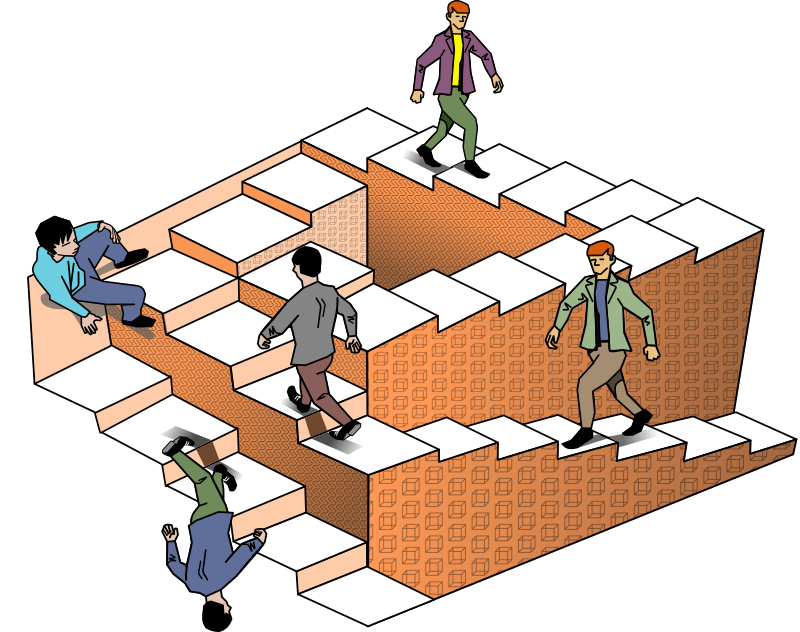
\includegraphics[width=0.50\textwidth]{stairs.png}
	\caption{Mynd í anda Escher fengin af openclipart.org}
	\label{fig: Escher}
\end{figure}

Reynum að átta okkur vel á þessu áður en við reynum að beita því.
Tökum aðeins óhlutbundnara dæmi.
Ímyndum okkur að börn standi í röð og bíði eftir fríum ís, manneskjan sem sér um ísinn snýr sér að fremasta barninu og segir ,,hvað viljiði marga íspinna?'', barnið vill einn en veit það ekki hvað hin börnin vilja svo það snýr sér að barninu fyrir aftan sig og segir ,,hvað vilt þú marga?'' það barn gerir það sama þangað til þau eru komin út í enda, það barn hefur ekkert annað barn til að spyrja og segir bara ,,tíu íspinna takk'', þá veit næst aftasta barnið að það séu allavega 10 íspinnar og svo 2 fyrir það sem þau vilja, og þannig leggjast tölurnar saman þar til fremsta barnið getur sagt ''59 íspinna takk fyrir okkur.''


\begin{wrapfigure}{o}{0.35\textwidth} %i o r l 
	\begin{center}
		
\includegraphics[scale=0.9]{doooodles_valborg-02.png}
	\end{center}
\end{wrapfigure}
Gott dæmi um hvernig megi beita endurkvæmni til að fá skilmerkilega niðurstöðu er að útfæra fall sem reiknar fyrir okkur einhver gildi í fibonacci röðinni.
En áður en við gerum það skulum við skoða enn einfaldara dæmi þar sem við erum með fall sem kallar í sig sjálft og gerir ekkert annað en það.
Í kóðabút \ref{lst:reiknirit-endurkvæmni1} sjáum við einfalda útgáfu af endurkvæmni, þar sem hugmyndin er í raun kynnt án þess að fallið sé neitt gagnlegt.
Það eina sem fallið gerir er að athuga hvort að tala sé stærri en núll og ef hún er það þá kallar fallið í sig sjálft með gildi sem er einum lægra, annars ef talan er ekki stærri en núll prentast ,,við kunnum á endurkvæmni''.
Hveru oft ætli það prentist ef við setjum inn töluna 5?

\begin{lstlisting}[caption=Endurkvæmni - einfalt, label=lst:reiknirit-endurkvæmni1]
def endurkvæmt_fall(tala):
	if(tala > 0):
		# á meðan talan er hærri en 0 þá köllum við aftur í fallið
		# en við köllum í það af gildi einu lægra
		return endurkvæmt_fall(tala-1)
	else:
		# hér erum við komin niður í 0 og prentum eftirfarandi texta
		print('við kunnum endurkvæmni')
		
endurkvæmt_fall(5)
\end{lstlisting}
\lstset{style=uttak}
\begin{lstlisting}
við kunnum endurkvæmni
\end{lstlisting}
\lstset{style=venjulegt}

Við sjáum í kóðabút \ref{lst:reiknirit-endurkvæmni1} að þó að við kölluðum í fallið með tölunni 5 þá fengum við bara einu sinni út strenginn ,,við kunnum endurkvæmni''.
Það er vegna þess að við kölluðum í fallið fyrir fimm og það sem fallið gerir fyrir okkur er að klára endurkvæmnina fyrir það kall, það verða ekki til fjögur önnur köll.
Heldur verður fimm að fjórum sem skilar okkur svo niðurstöðunni fyrir þrjá og svo koll af kolli þar til við erum komin niður í núll og þá hættir reikniritið keyrslu.
Í þessu tilfelli skilar það engu til baka upp fallakallið en klárast engu að síður þarna í línu 8 þegar það kemst þangað.


Það sem þetta reiknirit okkar gerir ekki er að skila einhverri niðurstöðu til baka, en nú skulum við skoða endurkvæmt reiknirit sem skilar summu í  \ref{lst:reiknirit-endurkvæmni-summa}.
Það reiknar summu af einhverri tölu og öllum jákvæðum tölum lægri en henni, svo talan 5 gæfi útkomuna 5 + 4 + 3 + 2 + 1 sem er 15.
Endurkvæmnin er því fólgin í því að upphaflega fallakallið með summa(100) skilar okkur 100 + summa(99), sem skilar okkur 100 + 99 + summa(98) og svo koll af kolli þar til talan 1 fæst, og við fáum útreikninginn 100 + 99 + ... + 1 sem skilar okkur 5050.

Einnig skulum við skoða fall sem reiknar n-tu töluna í fibonacci rununni.
Endurkvæmnin í fib(4) er fólgin í því að skoða alltaf tvær summur í einu en þær skila sér í sama fallakallið.
Svo fib(4) skila því sem fib(2) + fib(3) skila.
Kóðann má sjá í kóðabút \ref{lst:reiknirit-endurkvæmni-fib} og á mynd \ref{fig:reiknirit-fib}, nú erum við ekki lengur að skila einu gildi og hala af útreikningi heldur erum við að skila tveimur hölum.

\begin{figure}
	\begin{center}
		
		\begin{tikzpicture}[level distance=10mm]
			\tikzstyle{level 1}=[sibling distance=20mm]
			\tikzstyle{level 2}=[sibling distance=10mm]
			\tikzstyle{level 3}=[sibling distance=10mm]
			\node at (0,0) {$f_4$}
			child { node {$f_3$}
				child { node {$f_2$}
					child { node {$f_1$} }
					child { node {$f_0$} }
				}
				child { node {$f_1$} }
			}
			child { node {$f_2$}
				child { node {$f_1$} }
				child { node {$f_0$} }
			};
		\end{tikzpicture}  
	\end{center}
\label{fig:reiknirit-fib}
	\caption{hér sést hvernig fibonacci fallið kallar alltaf í tvö gildi. Svo eru neðstu gildin, gildin sem vísa ekki í neitt annað, þau sem leggjast saman.}
\end{figure}

\phantom{easter egg}
%\begin{wrapfigure}{i}{0.2\textwidth} %i o r l 
	\begin{center}
		
\includegraphics[scale=0.9]{doooodles_valborg-02.png}
	\end{center}
%\end{wrapfigure}


\begin{lstlisting}[caption=Summa reiknuð endurkvæmt, label=lst:reiknirit-endurkvæmni-summa]
def summa(n):
	if n <= 1:
		return 1
	else:
		return n + summa(n-1)

summa(6)
\end{lstlisting}
\lstset{style=uttak}
\begin{lstlisting}
21
\end{lstlisting}
\lstset{style=venjulegt}

\begin{lstlisting}[caption=Fibonacci tölur reiknaðar endurkvæmt, label=lst:reiknirit-endurkvæmni-fib]
def fib(n):
	if n <= 1:
		return n
	else:
		return fib(n-2) + fib(n-1)

fib(4)
\end{lstlisting}
\lstset{style=uttak}
\begin{lstlisting}
3
\end{lstlisting}
\lstset{style=venjulegt}

%\begin{wrapfigure}{i}{0.2\textwidth} %i o r l 
	\begin{center}
		
\includegraphics[scale=1.9]{doooodles_valborg-02.png}
	\end{center}
%\end{wrapfigure}

Nú höfum við séð lykkju útfærslu á helmingunarleit sem keyrir á meðan við höfum bil til að leita á en nú skulum við skoða hvernig megi gera þetta endurkvæmt.

\begin{lstlisting}[caption=Helmingunarleit að tölu í röðuðum lista með endurkvæmni, label=lst:reiknirit-helm-end]
def helmingunarleit_med_endurkvaemni(listi, vinstri, haegri, x): 
	# Endurkvæmt fall sem skilar sætisvísinum sem x finnst í í listanum listi
	# Ef x er ekki að finna í listanum listi þá fæst -1
	
	# Athugum hvort að vinstri sé enn vinstra megin
	if haegri >= vinstri: 
	
		# Stillum miðjuna
		midjan = int((vinstri + haegri)/2)
		#midjan = math.floor(vinstri + (haegri - vinstri)/2)
		
		# Athugum hvort gildið sé í miðjustakinu
		if listi[midjan] == x: 
			return midjan 
		
		# Ef gildið er lægra en miðjan þá þurfum við að leita frá vinstri að miðju
		elif listi[midjan] > x: 
			return helmingunarleit_med_endurkvaemni(listi, vinstri, midjan-1, x) 
	
		# Annars hlýtur gildið að vera frá miðju að hægra gildi
		else: 
			return helmingunarleit_med_endurkvaemni(listi, midjan+1, haegri, x) 
	
	else: 
		# Nú er hægra orðið minna en vinstra svo að
		# við erum búin að leita af okkur allan grun
		# gildið er ekki í listanum
		return -1
\end{lstlisting}

%\subsection{Bubble sort}\index{Bubble sort}\label{uk:reiknirit-bubble}
%Nú þegar við höfum leyst það hvernig á að leita að tölu á bili ef bilið er raðað, þá er mikilvægt að skoða hvernig er eiginlega hægt að raða?

%Við höfum séð að listar, innbyggða gagnatagið í Python, hefur innbyggðu aðferðina sort().
%Það sem sort gerði var að breyta lista fyrir okkur þannig að hann væri raðaður í vaxandi röð.

%Nú viljum við hinsvegar átta okkur á því hvernig við getum útfært reiknirit sem raðar fyrir okkur stökum í lista.


%-------------------------------
\newpage
\section{Æfingar}
\begin{exercise}\label{rei1}
Búið til fall sem tekur við tveimur hnitum, x og y gildum.
Það sem fallið á að gera er að skila tölu byggt á því hversu margar hreyfingar hrókur, taflmaðurinn, þyrfti að fara til að komast úr einu hniti í annað.
Í boði eru þrír möguleikar, tvær, ein eða engin hreyfing.

Gerum ráð fyrir að öll möguleg rauntöluhnit séu lögleg fyrir þennan ofurhrók.
\end{exercise}
\setboolean{firstanswerofthechapter}{true}
\begin{Answer}[ref={rei1}]
	\begin{lstlisting}
def hnit(hni11, hnit2):
	# gert er ráð fyrir að hnit sé annað hvort nd eða listi
	if(hnit1 == hnit2):
		return 0
	if(hnit1[0] == hnit2[0] or hnit1[1] == hnit2[1]):
		return 1
	else:
		return 2\end{lstlisting}
\end{Answer}
\setboolean{firstanswerofthechapter}{false}

\begin{exercise}\label{rei2}
Við viljum geta sagt til um hvaða leið er styst og hver er lengst, gefið er ákveðin lestarleið í formi lista af tölum.
Tölurnar tákna hversu langt stoppin eru frá upphafstöðinni.
Þið eigið annars vegar að búa til fall sem tekur við lista og skilar stystu fjarlægð milli tveggja nærliggjandi stöðva og hins vegar eigið þið að búa til fall sem tekur við sambærilegum lista en skilar lengstu fjarlægð milli tveggja nærliggjandi stöðva.

Athugið að fyrir listann \texttt{[1,3,7,19]} væri svarið 2 fyrir fyrra fallið en 12 fyrir seinna fallið.
Athugið hér sérstaklega bubblesort og hvernig á að skoða tvö stök í einu.
\end{exercise}
\begin{Answer}[ref={rei2}]
Hér er mikið atriði að prófa allskonar mismunandi lista til að vera viss um að þið séuð með kórréttan kóða.
	\begin{lstlisting}
def minnsta_fjarl(listi):
	styst = abs(listi[1]-listi[0])
	for i in range(len(listi)-1):
		if(styst > abs(listi[i+1]-listi[i])):
			styst = abs(listi[i+1]-listi[i])
	return styst

def mest_fjarl(listi):
	mest = abs(listi[1]-listi[0])
	for i in range(len(listi)-1):
		if(mest < abs(listi[i+1]-listi[i])):
			mest = abs(listi[i+1]-listi[i])
	return mest

\end{lstlisting}
\end{Answer}

\begin{exercise}\label{rei2}
Búið til fall sem spyr notandann um fjölda barna sem eru að biðja um íspinna, innan þess falls skulið vera með fall sem endurkvæmt reiknar út summu íspinna sem börnin vilja.
Notið random kóðasafnið til að búa til einhvern fjölda íspinna sem hvert barn vill.
\end{exercise}
\begin{Answer}[ref={rei2}]
Hér gætum við að notað input fallið og randint
	\begin{lstlisting}
import random as rnd
def ispinnar():
	def summa(fjoldi):
		if fjoldi <= 1:
			return 10
		else:
			return rnd.randint(0,10) + summa(fjoldi - 1)

	fjoldi = input('Hvað eru mörg börn í röðinni? ')
	try:
		int(fjoldi)
		return summa(int(fjoldi))
	except:
		return 10
	\end{lstlisting}
\end{Answer}

%\chapterimage{chapters17.png} % Chapter heading image

\chapter{Hugbúnaðarþróun}\index{Hugbúnaðarþróun}\label{k:dev}
Eins og fram kom í síðasta kafla þá snýst endirinn á þessari bók um framhaldið fyrir nema sem vilja leggja land undir fót í tölvunarfræðum.
Þessi kafli er þó meira í anda hugbúnaðarverkfræði en tölvunarfræði.

Það kemur nefnilega mörgum á óvart hvað góð samskipti eru stór hluti af því að þróa hugbúnað, forhugmyndir um fólk sem situr eitt við tölvuna sína og gerir eitthvað alveg af sjálfdáðum eru sterkar.

Hugmynd þarf einhvern veginn að verða að veruleika og það má vel vera að hugmynd að góðum og nothæfum hugbúnaði hafi sprottið upp hjá einum einstaklingi en flestur hugbúnaður sem við notum í dag, eins og forrit í símum, eru yfirleitt ekki hönnuð, forrituð, prófuð og markaðssett af einni manneskju.
Þess vegna er þess virði að taka fyrir stuttan kafla um hvað felst í hugbúnaðarþróun.

Áður en lengra er haldið er þó rétt að taka fram að það er engin ein ,,rétt“ leið til að þróa hugbúnað, fólk verður að prófa sig áfram til þess að finna hvað hentar.

\section{Útgáfustjórnun}\index{Útgáfustjórnun}
Fyrir það fyrsta er \textbf{útgáfustjórnun} (e. version control) nauðsynleg.
Ekki bara mikilvæg, nauðsynleg.
Til er hellingur af lausnum, opinn hugbúnaður sem og lokaður, sem sinnir þessu mikilvæga hlutverki.

Útgáfustjórnun kannast kannski sum við sem hafa notfært sér Word úr Office pakkanum, að geta rúllað til baka í einhverja útgáfu af tilteknu skjali þegar það skemmist eða gögn tapast skyndilega.
Það er í raun allt og sumt.
Að geyma kóðann á bak við hugbúnaðinn þar sem hver sem á að hafa aðgang hefur viðeigandi aðgang.\footnote{Viðeigandi aðgangur gæti t.d. verið skrifréttindi og lesréttindi, að þau sem þurfa ekki að geta breytt neinu heldur geti bara lesið og þau sem eiga að geta gert breytingar hafi réttindi til að skrifa.}

Burtséð frá aðgangsmálum er útgáfustjórnun falin í því að gera litlar breytingar því stór jafnt sem lítil kerfi geta verið brothætt og því mikilvægt að geyma þær breytingar sem við gerum í litlum skrefum svo hægt sé að snúa við og hætta notkun einhverra breytinga sem kom í ljós að hafa valdið villum.
Einnig gerir útgáfustjórnun \textit{kóðarýni} (e. code review) auðveldari.
Kóðarýni er mikivægur hluti af hugbúnaðarþróun, þar sem einhver er fenginn til að fara yfir kóða frá öðrum og finna hvað mætti betur fara.

Þessi bók var skrifuð með aðstoð git útgáfustjórnunartólsins og gitbub hýsingaraðilans.
Fleiri góð tól eru til eins og Bitbucket, SVN, Mercurial og önnur sem eru innbökuð í hugbúnaðarþróunartól (e. IDE eða integrated development environment) eins og VisualStudio.
Aðalatriðið í vali á tóli fyrir útgáfustjórnunina er að það henti öllum þeim sem eiga að koma að þróuninni, passi við þau stýrikerfi sem fólk notar og best er ef fyrri reynsla er góð.

\section{Stefnur og straumar}\index{Stefnur og straumar}
Alls konar hugmyndafræði hefur legið til grundvallar við gerð hugbúnaðar og stórra kerfa.
Til eru nokkuð stórar stefnur innan hugbúnaðarþróunar og er ein vinsælasta hugmyndafræðin kvik þróun eða agile, sem fær sinn eigin undirkafla.
En það þýðir ekki að það séu ekki til fleiri aðferðafræðir og í flestum þeirra er teymisvinna forritara hornsteinninn.

Þegar hugbúnaður var fyrst þróaður á 20. öldinni voru verkfræðingar og stærðfræðingar í fararbroddi.
Því þarf ekki að koma á óvart að verkfræðileg nálgun varð vinsæl stefna í þróun hugbúnaðar, sú sem mest var beitt heitir \textit{fossalíkanið} (e. waterfall model).
Fossalíkanið byggir á því að komast að því hverjar þarfir og skorður eru á verkefninu, hanna út frá því vöru og prófa hana svo, afurðin er fullbúin vara.
Þessi hugmyndafræði virkar fyrir hin ýmsu verkefni þar sem hægt er að komast að skorðum og þörfum á mjög hnitmiðaðan, skýran og óyggjandi máta.
Eftir því sem notendur fengu meira vægi þurfti að gera breytingar á því hvernig hugbúnaður var þróaður og fékk önnur hugmyndafræði að ryðja sér til rúms, \textit{samfelld þróun} (e. continuous development) þar sem stöðugt var verið að líta til baka og gera breytingar (þetta mun hljóma afskaplega svipað agile en það eru þó einhverjir megindrættir sem eru ólíkir). 

Eftir því sem fleiri fóru að þróa hugbúnað eftir að líða tók á öldina komu sífellt fleiri hugmyndafræðilegir ágreiningar í ljós.
Önnur hugmyndafræði sem naut mikilla vinsælda var \textit{prófunarþróun} (e. test driven development eða TDD) sem er enn þá við lýði í dag.
Hún snýst um að stöðugt má prófa skorður og þarfir og prófanirnar sýna að hugbúnaðurinn stenst þær kröfur sem hann á að standast.
Gallinn við þá nálgun er að prófanirnar eru mögulega ekki nógu yfirgripsmiklar og eitthvað lendir á milli og gleymist.

\section{Kvik þróun - agile}\index{Kvik þróun - agile}
Kvik þróun fær ekki sérkafla til að setja hugmyndafræðina á einhvern stall heldur því hún er svo ótrúlega vinsæl.
Kvik þróun hefur verið notuð bæði sem haldbær þróunaraðferð en einnig sem \textit{tískuorð} (e. buzz word).

Agile snýst um samfelldan þróunarferil þar sem litlar breytingar eru teknar inn á afmörkuðu tímabili.
Þessi tímabil eru kölluð \textit{sprettir} (e. sprints) og eru endurtekin þar til hugbúnaðinum er skilað (nema auðvitað honum sé viðhaldið).
Afurðin er því oftast enn í vinnslu þó henni sé sleppt í hendur notenda.

Grunnurinn byggir á fjórum hornsteinum:
\begin{itemize}
	\item Einstaklingar ofar tólum.
	\item Hugbúnaður sem virkar ofar yfirgripsmikilli skjölun.
	\item Samskipti ofar samningum.
	\item ,,Viðbregðni“ ofar því að fylgja plani.
\end{itemize}

Ásamt þessum hornsteinum eru tólf grunngildi sem snúa að því hvernig eigi að vinna sem teymi, líta til baka og gera endurbætur.

Þessar grunnhugmyndir eru nokkuð opnar sem hefur leitt til þess að til eru nokkuð mörg \textit{afbrigði} (e. flavor) af Agile hugmyndafræðinni.
Öll afbrigðin eiga það sameiginlegt að taka hornsteinana frekar heilaga en leggja áherslur hver á sín grunngildi eða túlka þau mismunandi.

Helstu afbrigði sem ber að nefna eru SCRUM, XP og Kanban.
Í SCRUM (sem er ekki stytting á neinu, en er þó alltaf skrifað í hástöfum) er alltaf lögð mikil áhersla á hin ýmsu hlutverk þróunarferlisins.
XP stendur fyrir ,,extreme programming“ og byggist á því að fólk vinni mjög náið saman, helst tvö eða fleiri á einni tölvu.
Kanban er ákveðið vinnuflæðirit sem má nýta með SCRUM og XP en einnig sem frjálslega útfærslu við Agile hugmyndafræðina.

Ástæða fyrir því að Agile er stundum notað sem tískuorð er sú að þessi hugmyndafræði er það vinsæl að flest fyrirtæki vilja segjast hafa tileinkað sér hana.
Þau hafa þó ekki öll gert það, það er engin vottun til fyrir slíkt og eru dæmi um fyrirtæki sem segjast vera kvik en það tekur heilt ár fyrir starfsfólk að skrá sig úr mötuneytisáskrift.

\section{Að lokum}\label{Að lokum}

Nú þegar við höfum náð góðum tökum á grunninum í forritun í Pyhton og skoðað við hverju má búast ef farið er lengra er hægt að líta til annarra mála eða frekari notkunar Python fyrir ákveðin verkefni.
Þá er gott að skoða pip, PyPI, git og Gihub.

Mikið er um góð námskeið og kennsluefni á netinu, eins og á Udemy, Khan Academy, Codewars, Codecombat og svo er ýmislegt að finna á Youtube.

Ekki hika við að gera mistök, þannig verðið þið betri í því sem þið takið ykkur fyrir hendur. 

	\begin{center}
		
\includegraphics[scale=5.9]{doodles31-02.png}
	\end{center}

\section{Exercises}\index{Exercises}

This is an example of an exercise.

\begin{exercise}
	This is a good place to ask a question to test learning progress or further cement ideas into students' minds.
\end{exercise}

%------------------------------------------------

\section{Problems}\index{Problems}

\begin{problem}
	What is the average airspeed velocity of an unladen swallow?
\end{problem}

\comment{

\chapter{Presenting Information}

\section{Table}\index{Table}

\begin{table}[h]
\centering
\begin{tabular}{l l l}
\toprule
\textbf{Treatments} & \textbf{Response 1} & \textbf{Response 2}\\
\midrule
Treatment 1 & 0.0003262 & 0.562 \\
Treatment 2 & 0.0015681 & 0.910 \\
Treatment 3 & 0.0009271 & 0.296 \\
\bottomrule
\end{tabular}
\caption{Table caption}
\label{tab:example} % Unique label used for referencing the table in-text
%\addcontentsline{toc}{table}{Table \ref{tab:example}} % Uncomment to add the table to the table of contents
\end{table}

Referencing Table \ref{tab:example} in-text automatically.

%------------------------------------------------

\section{Figure}\index{Figure}

\begin{figure}[h]
\centering
\includegraphics[scale=0.5]{placeholder.jpg}
\caption{Figure caption}
\label{fig:placeholder} % Unique label used for referencing the figure in-text
%\addcontentsline{toc}{figure}{Figure \ref{fig:placeholder}} % Uncomment to add the figure to the table of contents
\end{figure}

Referencing Figure \ref{fig:placeholder} in-text automatically.

}

%----------------------------------------------------------------------------------------
%	BIBLIOGRAPHY
%----------------------------------------------------------------------------------------
\comment{


\chapter*{Bibliography}
\addcontentsline{toc}{chapter}{\textcolor{ocre}{Bibliography}} % Add a Bibliography heading to the table of contents

%------------------------------------------------

\section*{Articles}
\addcontentsline{toc}{section}{Articles}
\printbibliography[heading=bibempty,type=article]

%------------------------------------------------

\section*{Books}
\addcontentsline{toc}{section}{Books}
\printbibliography[heading=bibempty,type=book]

}

\part{Lausnir}

\chapterimage{chapters7.png} % Chapter heading image

\chapter{Lausnir verkefna}\index{Lausnir verkefna}\label{Lausnir}

\shipoutAnswer


\chapterimage{chapter_head_2.pdf} % Chapter heading image

\chapter{Lausnir - strengir}\index{Lausnir - strengir}
\comment{
\chapterimage{chapter_head_2.pdf} % Chapter heading image

\chapter{Lausnir - listar}\index{Lausnir - listar}
\chapterimage{chapter_head_2.pdf} % Chapter heading image

\chapter{Lausnir - segðir og sanngildi}\index{Lausnir - segðir og sanngildi}
\chapterimage{chapter_head_2.pdf} % Chapter heading image

\chapter{Lausnir - lykkjur}\index{Lausnir - lykkjur}
\chapterimage{chapter_head_2.pdf} % Chapter heading image

\chapter{Lausnir - ndir}\index{Lausnir - ndir}
\chapterimage{chapter_head_2.pdf} % Chapter heading image

\chapter{Lausnir - orðabækur}\index{Lausnir - orðabækur}
\chapterimage{chapter_head_2.pdf} % Chapter heading image

\chapter{Lausnir - mengi}\index{Lausnir - mengi}
\chapterimage{chapter_head_2.pdf} % Chapter heading image

\chapter{Lausnir - föll}\index{Lausnir - föll}
\chapterimage{chapter_head_2.pdf} % Chapter heading image

\chapter{Lausnir - kóðasöfn}\index{Lausnir - kóðasöfn}
\chapterimage{chapter_head_2.pdf} % Chapter heading image

\chapter{Lausnir - skjalavinnsla}\index{Lausnir - skjalavinnsla}
\chapterimage{chapter_head_2.pdf} % Chapter heading image

\chapter{Lausnir - klasar}\index{Lausnir - klasar}
\chapterimage{chapter_head_2.pdf} % Chapter heading image

\chapter{Lausnir - villumeðhöndlun}\index{Lausnir - villumeðhöndlun}
\chapterimage{chapter_head_2.pdf} % Chapter heading image

\chapter{Lausnir - reiknirit}\index{Lausnir - reiknirit}
\chapterimage{chapter_head_2.pdf} % Chapter heading image

\chapter{Lausnir - hugbúnaðarþróun}\index{Lausnir - hugbúnaðarþróun}
}
%----------------------------------------------------------------------------------------
%	INDEX
%----------------------------------------------------------------------------------------

\cleardoublepage % Make sure the index starts on an odd (right side) page
\phantomsection
\setlength{\columnsep}{0.75cm} % Space between the 2 columns of the index
\addcontentsline{toc}{chapter}{\textcolor{ocre}{Index}} % Add an Index heading to the table of contents
\printindex % Output the index

%----------------------------------------------------------------------------------------

\end{document}
